% Isharati — technical documentation. Compile with:  latexmk -xelatex main.tex   (or xelatex, bibtex, xelatex x2)
\documentclass[11pt,a4paper,oneside]{report}
\usepackage[margin=2.3cm]{geometry}
\usepackage{fontspec}
\usepackage{polyglossia}
\setmainlanguage{english}
\setotherlanguage{arabic}
\setmainfont{TeX Gyre Termes}
\newfontfamily\arabicfont[Script=Arabic,Scale=1.05]{Amiri}
\newfontfamily\arabicfontsf[Script=Arabic]{Noto Naskh Arabic}
\usepackage{amsmath,amssymb}
\usepackage{graphicx,xcolor,booktabs,tabularx,longtable,multirow,array,makecell}
\usepackage{caption,subcaption}
\usepackage{enumitem}
\usepackage{tikz}
\usetikzlibrary{positioning,arrows.meta,fit,backgrounds,shapes.geometric,calc}
\usepackage{listings}
\usepackage[hyphens]{url}
\usepackage[colorlinks=true,linkcolor=teal!70!black,citecolor=teal!70!black,urlcolor=teal!60!black,hyperfootnotes=false]{hyperref}
\usepackage{cite}
\usepackage{titlesec}
% each chapter opens with its name alone on a page
\titleformat{\chapter}[display]{\normalfont\centering\color{navy}}
  {\vspace*{0.30\textheight}{\Large\scshape\chaptertitlename\ \thechapter}}{14pt}
  {\rule{0.35\textwidth}{0.6pt}\\[12pt]\fontsize{30}{36}\selectfont\bfseries}
  [\vspace{10pt}\rule{0.35\textwidth}{0.6pt}\clearpage]
\titlespacing*{\chapter}{0pt}{0pt}{0pt}
\titleformat{\section}{\Large\bfseries\color{navy}}{\thesection}{0.7em}{}
\titleformat{\subsection}{\large\bfseries}{\thesubsection}{0.6em}{}
\setlength{\parskip}{3pt}
\captionsetup{font=small,labelfont=bf}
\definecolor{ink}{HTML}{1D1D1B}\definecolor{tealx}{HTML}{14B8A6}\definecolor{amberx}{HTML}{F59E0B}
\definecolor{navy}{HTML}{1E3A5F}\definecolor{soft}{HTML}{EEF7F6}
\newcommand{\ar}[1]{\textarabic{#1}}
\newcommand{\code}[1]{\texttt{\small #1}}
\usepackage{seqsplit}
\newcommand{\idcode}[1]{{\ttfamily\small\seqsplit{#1}}}
\newcolumntype{L}[1]{>{\raggedright\arraybackslash}p{#1}}
\newcolumntype{Y}{>{\raggedright\arraybackslash}X}
\lstset{basicstyle=\ttfamily\footnotesize,breaklines=true,frame=single,rulecolor=\color{gray!40}}
\urlstyle{same}

\title{\textbf{Isharati (\ar{إشارتي}): Grounded Sign Language Generation for Islamic Content}\\[4pt]
\large Technical Documentation --- Bathel AI Challenge 2026: Serving Islamic Content (Track 2)}
\author{Fatimah Emad Eldin \and Asmaa Al-Mirghani}
\date{October 2026}

\begin{document}
\maketitle

\begin{abstract}
\noindent Isharati is an AI-powered platform that brings the Qur'an and the Sunnah to Deaf and hard-of-hearing people in
their first language, sign language, and gives preachers and Islamic content creators integrated tools to reach them
without barriers. It answers a wide demographic and human need: more than 70 million Deaf people live worldwide (more
than 15 million of them Muslims), and they face a double linguistic and cultural isolation, because religious content
reaches them written or spoken in a language that is not theirs, while the signed content that exists is scarce,
scattered and without documented sources. Preachers, for their part, lack translation tools built for religious text:
tools that respect the precision of the scripture and avoid both unfounded interpretation and spelling Islamic terms
letter by letter instead of using their established signs.

To close this gap, Isharati brings education, answers and content creation together in one platform, built entirely
on documented sources. \emph{Verified question and answer} accepts a question in Arabic, English, Turkish or Urdu,
retrieves the relevant verses and hadith by retrieval-augmented generation (RAG), and accepts no sentence that its
source does not support; questions asking for a religious ruling are referred to scholars. The \emph{Academy} offers
interactive paths for learning the letters and religious terms in four sign languages, ending with a certificate of
completion, alongside a \emph{Qur'an and hadith corpus} of about 8,000 signed Qur'an segments (about 45 hours, from five
recognised sources such as the King Fahd Complex and the Al-Kharj curriculum) and more than 300 labelled hadith.

For institutions and preachers, the \emph{Content Studio} turns texts, audio or video lessons into signing at once,
with control over the signing speed, a choice of avatars in modest dress, and video export.

The sign lexicons cover most of the scripture: the share of content words in the Qur'an and hadith that the
lexicon of each language signs is 83.1\% for English to American Sign Language (3,677 signs), 75.7\% for Turkish to
Turkish Sign Language (4,827 signs), 72.9\% for Arabic to Arabic Sign Language (6,663 signs; 74.2\% with proper names
shown by fingerspelling), and 72.1\% for Urdu to Indian and Pakistani Sign Language (10,233 signs). Against the signs of
Deaf signers, the Arabic matcher chooses the right sign for 98.3\% of the words of religious sentences, with no wrong
sign.

Isharati thus offers a double value: direct and safe access for Deaf people to their religion at any time, and a
multiplied reach for preaching institutions at low cost and high efficiency. Its aim is that every Deaf Muslim receives
the Qur'an and the Sunnah as others do: understood, documented, and in their own language, so that Islamic content in
sign language becomes an integral part of preaching rather than an exception.
\end{abstract}

\begin{Arabic}
\noindent\textbf{الملخّص.}
تُعد «إشارتي» منصة رائدة مدعومة بالذكاء الاصطناعي تهدف إلى جعل القرآن الكريم والسنة النبوية في متناول الصم وضعاف
السمع بلغتهم الأم (لغة الإشارة)، مع منح الدعاة وصُنّاع المحتوى الإسلامي أدوات متكاملة تُمكّنهم من الوصول إلى هذه
الفئة دون حواجز. يأتي هذا الابتكار استجابةً لتحدٍ ديموغرافي وإنساني واسع؛ حيث يعيش أكثر من 70 مليون أصم حول العالم
(من بينهم أكثر من 15 مليون مسلم أصم)، يواجهون عزلة لغوية وثقافية مضاعفة نظراً لأن المحتوى الديني يصلهم مكتوباً أو
مسموعاً بلغة ليست لغتهم، فضلاً عن ندرة المحتوى الإشاري المتفرّق وافتقاره للمصادر الموثقة. وفي المقابل، يعاني الدعاة
من غياب أدوات الترجمة المتخصصة التي تحترم دقة النصوص الشرعية وتتجنب مخاطر الاجتهاد الخاطئ أو تهجئة المصطلحات حرفياً
بدل إشاراتها المعتمدة.

ولسد هذه الفجوة الهيكلية، تجمع منصة «إشارتي» في بيئة رقمية واحدة حلولاً مبتكرة للتعليم، والإجابة، وصناعة المحتوى
استناداً إلى مصادر موثقة بالكامل. تتضمن المنصة ميزة «سؤال وجواب موثق» التي تتيح للمستخدم الاستعلام بلغات متعددة
(العربية، الإنجليزية، التركية، الأردية) لتسترجع المنصة الآيات والأحاديث ذات الصلة عبر تقنية التوليد المعزز
بالاسترجاع (RAG) دون أي قبول لجملة لا يدعمها مصدرها، مع إحالة أسئلة الفتوى تلقائياً لأهل العلم. كما توفر «الأكاديمية»
مسارات تفاعلية لتعليم الحروف والمصطلحات الدينية بأربع لغات تنتهي بشهادة إتمام، إلى جانب «مدونة القرآن والحديث» التي
تضم نحو 8,000 مقطع قرآني (قرابة 45 ساعة من خمسة مصادر معتمدة كَمجمع الملك فهد ومنهج الخرج) وأكثر من 300 حديث نبوي
موسوم.

ولتمكين المؤسسات والدعاة، تقدم المنصة «استوديو صناعة المحتوى» الذي يتيح تحويل النصوص أو الدروس الصوتية والمرئية إلى
إشارة فورية مع التحكم في سرعة الأداء واختيار الشخصيات الافتراضية ذات الزي المحتشم وتصدير الفيديو بسلاسة.

وتغطي المعاجم الإشارية معظم النصوص الشرعية: إذ تبلغ نسبة الكلمات ذات المعنى في القرآن والحديث التي يملك معجم كل لغة
إشارةً لها \textenglish{83.1\%} للإنجليزية إلى لغة الإشارة الأمريكية (3,677 إشارة)، و\textenglish{75.7\%} للتركية إلى لغة الإشارة التركية (4,827
إشارة)، و\textenglish{72.9\%} للعربية إلى لغة الإشارة العربية (6,663 إشارة؛ و\textenglish{74.2\%} مع عرض أسماء الأعلام بالتهجئة الإشارية)، و\textenglish{72.1\%}
للأردية إلى لغة الإشارة الهندية والباكستانية (10,233 إشارة). ومقارنةً بإشارات مترجمين صمّ فعليين، يختار النظام
العربي الإشارة الصحيحة لـ\textenglish{98.3\%} من كلمات الجمل الدينية دون أي إشارة خاطئة.

وبذلك تقدم «إشارتي» قيمة مضاعفة تتمثل في وصول مباشر وآمن للصم إلى دينهم في أي وقت، ومضاعفة الأثر الدعوي للمؤسسات
بتكلفة منخفضة وكفاءة عالية، لتسعى المنصة في النهاية إلى أن يتلقى كل أصم مسلم القرآن والسنة كما يتلقاهما غيره:
مفهومان، موثقان، وببلغته، ليصبح المحتوى الإسلامي الإشاري جزءاً أصيلاً من العمل الدعوي لا استثناءً.
\end{Arabic}

\noindent\textbf{Keywords:} sign language, Arabic Sign Language, American Sign Language, retrieval-augmented generation,
Qur'an, hadith, accessibility, Deaf Muslims, 3D avatar.

\tableofcontents
\newpage
\chapter{Introduction}
\label{sec:intro}

\section{Motivation}
More than 70 million deaf people use a sign language as their first language, across more than two hundred
national sign languages \cite{wfd,unsign}, and the World Health Organization projects that by 2050 one in four people
will live with some degree of hearing loss \cite{whoasl}. For many deaf Muslims the written language of the
Qur'an and of hadith collections is a second language: Arabic text, even in translation, is not the language in which
they think and ask questions. Interpreters who know both a sign language and Islamic terminology are rare, and the
content that does exist in sign language is scattered across short videos of uneven quality, without sources. The
contrast with other traditions is stark: Bible translations in 98 sign languages, 2,530 hours by more than 1,500
signers, are already a machine-learning corpus \cite{jwsign}, while for the Qur'an and hadith we found no aligned corpus
in any sign language (Chapter~\ref{sec:related}). Signed hadith do exist, as several hundred videos by Deaf associations
and educational channels, but none is aligned to the hadith text or usable by a model (Chapter~\ref{sec:scripture}). A deaf Muslim who asks a question about the faith should be able to
receive an answer in their own language, taken from the sources and not from a guess.

\paragraph{The Congregational Dilemma and the Medina Precedent.}
In physical worship, Deaf Muslims regularly attend the five daily prayers and the weekly Friday \textit{Juma'a} gathering, standing shoulder-to-shoulder in prayer ranks (\textit{sufuf}) alongside hearing worshippers. Yet, they endure complete linguistic and cognitive isolation: the imam's melodic Qur'anic recitation, the Friday sermon (\textit{khutbah}), theological admonitions, and communal supplications remain entirely inaudible. While appearing physically integrated, Deaf congregants silently blend into the congregation without comprehending the guidance being delivered.

A commendable institutional benchmark exists at the Prophet's Mosque (\textit{Al-Masjid an-Nabawi}) in Medina, where the General Presidency operates a dedicated hall equipped with closed-circuit television displays and on-site certified human sign language interpreters who translate the Friday khutbah live. While this sanctuary model serves as a vital proof-of-concept, it relies on centralized state resources and full-time certified human interpreters (\$50--\$120/hour) who are in desperately short supply. As a result, this model cannot scale to the more than 100,000 neighborhood and regional mosques across Saudi Arabia, Egypt, Syria, the Gulf, and the wider Muslim world. To eliminate this barrier universally, an automated, low-latency pipeline capable of converting live imam speech into morphologically faithful sign language is urgently required.

\section{Problem statement}
Machine sign language production (SLP) has made progress on general domains \cite{progressivetransformers,text2sign,
slpreview,slpsurvey,signllm,slrtp2025}, but religious content and sacred congregational settings raise three critical requirements that general systems do not meet:
\begin{enumerate}[leftmargin=*,itemsep=1pt]
  \item \textbf{Faithfulness.} An answer about the Qur'an or the Sunnah must not add facts, rulings or attributions.
        A fluent but invented statement attributed to the Prophet \ar{ﷺ} is worse than no answer.
  \item \textbf{Correct signs for Islamic terms.} Words such as \emph{salah}, \emph{zakah}, \emph{Hajj} or
        \ar{محمد رسول الله} have established signs in each sign language; spelling them letter by letter
        (fingerspelling) is not acceptable to the community, and a wrong sign changes the meaning.
  \item \textbf{Live congregational speech-to-sign integration.} Live Friday sermons and madrasah lectures are delivered orally in acoustic environments that exclude Deaf worshippers. Scaling accessibility beyond premier sanctuaries like Medina requires real-time automatic speech recognition (ASR) coupled with Semitic morphological gloss synthesis and zero-cost client 3D avatar rendering, deployable in standard local mosques without requiring human interpreters or dedicated television production studios.
\end{enumerate}

\section{Objectives}
\begin{enumerate}[label=\textbf{O\arabic*.},leftmargin=*,itemsep=1pt]
  \item \textbf{Comprehensive sign language toolkit.} Build an end-to-end open-source toolkit and interactive platform supporting bidirectional translation, content generation, Qur'an recitation, and grounded Q\&A in sign languages.
  \item \textbf{Signs for Islamic vocabulary.} Assemble sign lexicons from public sources, in one standardized pose format, for the
        sign languages of the English, Arabic, Turkish and Urdu modes, with Islamic terms signed, never fingerspelled.
  \item \textbf{Grounded Islamic generation.} Answer questions about Islam strictly from the Qur'an and authenticated hadith, with every
        sentence traceable to a cited passage, verbatim verse quotation, and automatic referral of fatwa/ruling queries to scholars.
  \item \textbf{High-fidelity signed production.} Render sign pose sequences as joint skeletons and customizable 3D VRM
        avatars with culturally appropriate modest-dress options (hijab, shemagh, and thobe).
  \item \textbf{Continuous pose segmentation and alignment.} Integrate pre-trained deep sequence models (RoPE Transformer) to segment continuous signing streams into discrete word gestures and align narrative scripture without speech dependency.
  \item \textbf{Empirical coverage and verification.} Quantify lexicon coverage across scripture corpora, provide automated weakly supervised sign mining, and establish rigorous evaluation benchmarks (support checking, gloss error rate, back-translation).
\end{enumerate}

\section{Proposed solution}
Isharati (\ar{إشارتي}, ``my sign'') is a comprehensive, open-source AI toolkit and multimodal platform for Islamic content generation, bidirectional translation, Qur'an recitation, and grounded question answering in sign languages. Rather than a simple Q\&A chatbot, Isharati provides a modular production engine and developer ecosystem designed to eliminate the severe accessibility gap faced by Deaf Muslims.

The platform unites four tightly integrated capabilities:
\begin{enumerate}[leftmargin=*,itemsep=1pt]
  \item \textbf{Multimodal Content Studio and Translation}: Users can input spoken text to generate natural sign language sequences, translate between sign glosses and natural text, or synthesize custom signed content with frame-level keypoint editing.
  \item \textbf{Grounded Theological Q\&A Engine}: Questions are answered using \emph{retrieval-augmented generation} (RAG)~\cite{rag} across the canonical Qur'an and authenticated hadith collections (HadeethEnc). A verification layer enforces per-sentence passage support and verbatim citation fidelity, while ruling requests (\emph{fatwa}) are referred to accredited scholars.
  \item \textbf{Continuous Signed Qur'an and Tafsir System}: A dedicated recitation module providing verse-by-verse signed interpretations across three major institutional corpora (King Fahd Complex, Al-Mukhtasar fi Tafsir, and the Al-Kharj curriculum), directly rendered on 3D avatars alongside side-by-side video alignments.
  \item \textbf{3D Avatar and Skeletal Production Engine}: Poses are projected onto customizable 3D VRM avatars with diverse modest-dress options (hijab, shemagh, and thobe) as well as skeletal overlays, featuring variable playback speeds and video export.
\end{enumerate}
The platform operates across four languages and sign traditions: American Sign Language (ASL, English mode), Arabic Sign Language (ArSL, Arabic mode), Turkish Sign Language (T\.{I}D, Turkish mode), and Indian Sign Language (ISL, standing in for Urdu), with full web deployment on Hugging Face Spaces and accessible REST APIs.

\section{Contributions}

To address the profound accessibility and resource gap for the global Deaf Muslim community, this work delivers the following pioneering theoretical, technical, and open-source contributions:

\begin{enumerate}[leftmargin=*,itemsep=4pt]
  \item \textbf{First-of-its-Kind Open-Source Bilingual Text-to-Sign Translation Suite}:
    While isolated text-to-sign tools have emerged for English in closed proprietary settings, Isharati introduces the \emph{first open-source, bidirectional neural text-to-sign (T2S) and sign-to-text (S2T) translation architecture} natively supporting both Arabic (Arabic Sign Language, ArSL) and English (American Sign Language, ASL), alongside extensible support for Turkish (T\.{I}D) and Urdu (ISL). The translation pipeline incorporates morphological clitic decomposition (via CAMeL Tools for Arabic and spaCy for English), syntactic gloss normalization, and cross-lingual pose alignment, enabling real-time conversion from natural spoken language directly into continuous 3D skeletal kinematic streams.

  \item \textbf{First Machine Learning Digitization of the Qur'an and Tafsir in Sign Language}:
    We establish the first structured, machine-learning-ready digital corpora of continuous sign language recitations and theological exegesis (*Tafsir*) for the Holy Qur'an. Sourced from three distinguished institutions, the recordings were extracted, anthropometrically normalized, and packaged into per-surah continuous 3D MediaPipe Holistic and 50-joint Isharati coordinates with smart kinematic hold-preservation envelopes:
    \begin{itemize}[leftmargin=*,itemsep=2pt]
      \item \textbf{King Fahd Glorious Qur'an Printing Complex (\code{kfc})}:
        Official continuous signed recitations and verse interpretations across Releases 1--6 (1,066 segments, 7.4\,hours of signing, 558 ayat of 38 Surahs):\\
        \url{https://huggingface.co/datasets/FatimahEmadEldin/quran-sign-kfc}
      \item \textbf{Al-Mukhtasar fi Tafsir (\code{mukhtasar})}:
        Comprehensive sign language exegesis spanning 112 Surahs (6,127 segments, 34.7\,hours of signing, 5,916 ayat):\\
        \url{https://huggingface.co/datasets/FatimahEmadEldin/tafsir-mukhtasar-sign}
      \item \textbf{Al-Kharj Educational Curriculum (\code{curriculum})}:
        Official pedagogical sign language curriculum covering 22 short Surahs for Deaf education (207 segments, 186 ayat):\\
        \url{https://huggingface.co/datasets/FatimahEmadEldin/quran-sign-curriculum}
      \item \textbf{Tebyan (\code{tebyan})} and \textbf{Diyanet (\code{diyanet}, Turkish Sign Language)}: publisher-labelled
        clips per ayah (567 segments, 570 ayat) and Diyanet's two Qur'an episodes (13 segments), labelled from the
        publisher's own text (Section~\ref{sec:quran_sets}).
    \end{itemize}

  \item \textbf{A Signed Hadith Corpus}:
    From 824 YouTube videos (114.4 hours) of hadith signed by Deaf associations and educational channels in ArSL and
    T\.{I}D, a corpus whose every label is the hadith as printed in its collection, never a transcript: 404 samples and
    15.4 hours in the 6 October 2026 snapshot, 351 of them verified against the collections, covering 282 distinct
    hadith and 41 of Nawawi's Forty, with keypoints, the signer's facial expression and a gloss target
    (Section~\ref{sec:hadith_corpus}):\\
    \url{https://huggingface.co/datasets/FatimahEmadEldin/hadith-sign}

  \item \textbf{Pose quality across the signed corpora}:
    An automatic check of every published sample found that all six signed datasets, and the lexicon, stored bodies
    stretched by the video's aspect ratio (upper arm 1.25--1.44 shoulder widths against an adult's 0.7--0.9); square
    units, a spike filter and a corrected reference body shape fix it (Section~\ref{sec:pose_qa}).

  \item \textbf{Broad Scripture Coverage Exceeding 70\% Across Arabic and English}:
    Through systematic linguistic evaluation against canonical Islamic scripture, we demonstrate that our harmonized sign lexicons cover \textbf{over 70\% of content-word occurrences} across both the Arabic Qur'an / Hadith and their standard English translations (66.5\% baseline ASL token coverage expanding to \textbf{83.1\%} via targeted vocabulary mining and reviewed synonyms, and Arabic content-word coverage of \textbf{72.9\%} with morphological lemma matching and reviewed synonyms; Turkish reaches 75.7\% and Urdu 72.1\% across all 6,236 Qur'anic ayahs and 5,902 HadeethEnc traditions).

  \item \textbf{End-to-End Deep Continuous Segmentation \& Quality Assurance}:
    We benchmark a pre-trained 2026 Rotary Position Embedding (RoPE) Transformer segmenter against velocity-minima and uniform-window heuristics on synthetic ArSL streams with exact boundaries and on Isharah, ArabSign, EGCBT and YouTube-ASL (Section~\ref{sec:results_segmentation}). No method is accurate yet: the best boundary F1 within $\pm4$ frames is 44.6\% (RoPE with the package's own preprocessing; velocity minima 40.1\%), the RoPE model through our app wrapper scores 6.5\%, and we found and fixed a label-decoding bug in that wrapper. The model runs at about 290 frames per second on a desktop CPU.

  \item \textbf{Weakly Supervised Sign Spotting \& Back-Translation Quality Assurance (Author Contribution)}:
    To resolve the long-tail problem of sacred Islamic vocabulary absent from standard conversational dictionaries, we trained a custom 5-layer dilated Temporal Convolutional Network (TCN) under a weakly supervised Multiple Instance Learning (MIL) objective across all 10 parts of the YouTube-ASL archive (357,022 captioned clips, over 21 million pose frames, with 14+ million frames in active training segments). Our spotter achieves a test mAP of \textbf{0.1135} ($60\times$ above the random baseline) and \textbf{0.2011} on held-out words, enabling automated back-translation verification and DTW consensus clustering that successfully mined and validated 153 missing scriptural signs into our ASL lexicon. We openly publish the trained model weights, architecture, and evaluation metrics:
    \begin{itemize}[leftmargin=*,itemsep=2pt]
      \item \textbf{YouTube-ASL MIL Sign Spotter (Ours)}:\\
        \url{https://huggingface.co/FatimahEmadEldin/youtube-asl-spotter}
    \end{itemize}
    Additionally, for reproducibility and open benchmarking in continuous pose-to-text translation, we re-packaged the fine-tuned sequence-to-sequence checkpoints (T5-Base, T5-v1.1-Base, and mT5-Base) originally released by the organizers of the Kaggle \emph{Saudi Sign For All Competition} (\url{https://www.kaggle.com/competitions/saudi-signfor-all-competition}) into standardized, drop-in Hugging Face model repositories with full inference code and tokenizers.

  \item \textbf{Production Multimodal Studio with Culturally Respectful 3D Avatars}:
    We deploy a full-featured web platform and developer API featuring: (a) deterministic citation verification and jurisprudential ruling guards (*fatwa referral*); (b) a synchronized dual-view video player matching human signers with 3D avatars; and (c) procedural modesty attire configurations for avatars (hijab, shemagh, and thobe), ensuring full cultural and religious alignment with Muslim Deaf communities worldwide.
\end{enumerate}


\section{Outcomes}
Measured against the objectives, the work to date achieves the following (Chapters~\ref{sec:eda}
and~\ref{sec:results}):
\begin{itemize}[leftmargin=*,itemsep=1pt]
  \item \textbf{O1.} Answers in English and Arabic are built only from cited verses and hadith; unsupported sentences are
        removed, and ruling questions are referred before any language model is called.
  \item \textbf{O2.} Lexicons of 3,055 ASL, 3,979 ArSL and 6,411 Indian Sign Language glosses, and a Turkish lexicon in
        progress (1,308 of 5,017 dictionary signs).
  \item \textbf{O3.} An end-to-end web application that signs answers with a skeleton or an avatar in three outfits
        (original, hijab, shemagh with thobe), at adjustable speed, with video export.
  \item \textbf{O4.} The ASL lexicon signs 66.5\% of the word occurrences of the English Qur'an and hadith (vocabulary
        without names); the 500 most frequent missing words would raise this to 87.6\%. The ArSL lexicon covers 59.6\%
        of Arabic word occurrences; the Turkish and Urdu lexicons, 16\% and 51\% of content words. In every language the
        largest gaps are the religious core and the hadith formulas, which a small set of phrase signs can close.
  \item \textbf{O5.} The Arabic glosser reaches a gloss WER of 0.52--0.55 against ArabSign's gold glosses on held-out
        sentences; a back-translation baseline is in place, and the stronger recognisers and the Deaf review are the
        next steps.
  \item \textbf{O6.} Five signed Qur'an datasets (7,980 segments, 44.9 hours) and a signed hadith corpus (404 samples,
        282 distinct hadith in the 6 October 2026 snapshot) are published, each segment linked to its source video,
        and served in the application's Sign Mushaf, Signed Hadith and Academy pages.
  \item \textbf{O7.} After the pose corrections every signed dataset is in the adult body range (upper arm 0.77--0.87
        shoulder widths), and the realistic avatars bend their elbows as the signer does (\ar{وضوء}: within
        0.3--4.1\textdegree{} of the signer, where they had been 44--74\textdegree{} too straight).
\end{itemize}

\section{Deliverables}
Table~\ref{tab:deliverables} enumerates the primary public deliverables, interactive systems, neural model checkpoints, and multimodal scripture datasets developed in this project, accompanied by their live access repositories.

\begin{table}[!ht]
\centering\footnotesize
\caption{System deliverables, open neural checkpoints, digital scripture corpora, and live repositories.}
\label{tab:deliverables}
\begin{tabularx}{\textwidth}{L{2.8cm} Y L{4.6cm} L{1.8cm}}
\toprule
\textbf{Deliverable} & \textbf{Description \& Technical Scope} & \textbf{Public Resource / Repository URL} & \textbf{Status} \\
\midrule
Interactive Web Studio & Full multimodal web application: real-time text-to-sign, grounded theological Q\&A, signed Qur'an recitation studio, 3D modest avatars (hijab, shemagh, thobe), and skeletal visualization. & \url{https://huggingface.co/spaces/FatimahEmadEldin/isharati-app} & Live Demo \\
\addlinespace[3pt]
MIL Sign Spotter \newline \emph{(Author Contribution)} & 5-layer dilated Temporal Convolutional Network (TCN) trained via Multiple Instance Learning on 357k YouTube-ASL clips for weakly supervised scriptural sign spotting and back-translation verification. & \url{https://huggingface.co/FatimahEmadEldin/youtube-asl-spotter} & Model Weights \\
\addlinespace[3pt]
Pose-to-Text Back-Translation Checkpoints & Fine-tuned sequence-to-sequence neural architectures (T5-Base, T5-v1.1-Base, and mT5-Base) standardized with inference tokenizers for continuous sign-to-text translation and QA evaluation. & \url{https://huggingface.co/FatimahEmadEldin/ytasl-t5-base} \newline \url{https://huggingface.co/FatimahEmadEldin/ytasl-mt5-base} & Model Weights \\
\addlinespace[3pt]
Continuous Sign Recognition (CSLR) & Conformer-based deep continuous sign language recognition model trained on the Isharah Arabic sign benchmark. & \url{https://huggingface.co/FatimahEmadEldin/cslr-conformer-isharah} & Model Weights \\
\addlinespace[3pt]
King Fahd Complex Signed Qur'an (\code{kfc}) & 1,066 continuous signed recitation and Tafsir segments across 104 Surahs (8.84 hours) extracted into normalized 50-joint 3D keypoints. & \url{https://huggingface.co/datasets/FatimahEmadEldin/quran-sign-kfc} & Open Dataset \\
\addlinespace[3pt]
Al-Mukhtasar fi Tafsir (\code{mukhtasar}) & 6,127 continuous signed theological exegesis segments across 112 Surahs (27.5 hours) with aligned verse transcriptions. & \url{https://huggingface.co/datasets/FatimahEmadEldin/tafsir-mukhtasar-sign} & Open Dataset \\
\addlinespace[3pt]
Al-Kharj Educational Curriculum (\code{curriculum}) & 207 pedagogical signed clips covering 22 short Surahs for Deaf education (1.25 hours) with 3D pose extraction. & \url{https://huggingface.co/datasets/FatimahEmadEldin/quran-sign-curriculum} & Open Dataset \\
\addlinespace[3pt]
Unified Multimodal Scripture Corpus & Complete 50-joint pose archive, 4-language harmonized lexicons (3,491 ASL, 6,610 ArSL, 6,411 ISL, 1,308 T\.{I}D), and canonical RAG scripture embeddings. & \url{https://huggingface.co/datasets/FatimahEmadEldin/isharati-data} & Open Dataset \\
\addlinespace[3pt]
Sign Annotation \& Review Studio Pool & 6,112 signs seeded across 12 dataset categories with Neon PostgreSQL review studio interface for Deaf community evaluation. & \url{https://huggingface.co/datasets/FatimahEmadEldin/isharati-review-signs} & Open Dataset \\
\addlinespace[3pt]
Open-Source Platform Codebase & Complete production implementation: FastAPI server, RAG retrieval engine, 3D VRM avatar runtime, and React landing page. & \url{https://github.com/astral-fate/isharati-signs} & Open Source \\
\bottomrule
\end{tabularx}
\end{table}

\section{Scope of this document}
This document describes the system as built and measured on 1--2 October 2026. Every number reported was measured on
the system and data described here; items that are planned but not yet measured are marked as such. Chapter~\ref{sec:discussion} lists the limitations, including the fact that no sign has yet been reviewed
by Deaf signers for this project.

\chapter{Background and related work}
\label{sec:related}

\section{Sign language processing tasks and how they are evaluated}
Sign language processing covers four related tasks that differ in their input, output and metric
(Table~\ref{tab:tasks}); a sign-generation system touches all four, because its own output can be checked only with the
recognition and translation tasks.

\begin{itemize}[leftmargin=*,itemsep=2pt]
  \item \textbf{Isolated sign recognition} is a classification task: one clip, one sign, scored by top-1 and top-5
        accuracy. WLASL \cite{wlasl}, MS-ASL \cite{msasl}, ASL Citizen \cite{aslcitizen}, KArSL \cite{karsl} and AUTSL
        \cite{autsl} are benchmarks of this kind, and their recordings are the raw material of sign lexicons.
  \item \textbf{Continuous sign recognition} maps a signed sentence to its \emph{gloss} sequence, the written labels of
        the signs in signing order. Models are trained with connectionist temporal classification (CTC) \cite{ctc},
        which needs only the gloss order, not the boundaries, and are scored by gloss word error rate (WER)
        \cite{koller2015,kollersurvey}. The best systems now reach low error rates on controlled data: the winning
        skeleton-based model of the ICCV 2025 multimodal sign language recognition challenge \cite{mslr2025,signeval2025}
        was trained on the Saudi Isharah dataset \cite{isharah}.
  \item \textbf{Sign language translation} maps a signed sentence to spoken-language text, with or without glosses as an
        intermediate step \cite{camgoz2018,signlanguagetransformers}. Because the target is free text, it is scored with
        machine translation metrics: BLEU \cite{bleu}, ROUGE \cite{rouge}, chrF \cite{chrf}, and learned metrics such as
        BLEURT \cite{bleurt} or BERTScore \cite{bertscore}. Large weakly aligned corpora such as YouTube-ASL
        \cite{youtubeasl} and How2Sign \cite{how2sign} pair sentences with video but have no glosses; pose-based
        translation on them has been studied in ablation \cite{t5slt}.
  \item \textbf{Sign language production} (SLP) is the reverse: text or gloss to a pose sequence or video. Progressive
        Transformers \cite{progressivetransformers} generate continuous skeleton sequences and introduced
        \emph{back-translation} evaluation: a translation model reads the generated pose, and its output is scored with
        BLEU and ROUGE against the source. Pose-level metrics such as DTW-MJE \cite{dtwmje} compare generated and
        reference joints. Text2Sign \cite{text2sign} combines translation with a motion graph and video generation, and
        SignLLM \cite{signllm} trains large multilingual production models. Surveys \cite{slpreview,slpsurvey,slpathways}
        and the SLRTP 2025 production challenge \cite{slrtp2025} report that generated signing still loses hand detail
        and that automatic metrics only partly agree with Deaf judges.
\end{itemize}

\begin{table}[ht]
\centering\small
\caption{Sign language processing tasks, their standard metrics, and their role in Isharati.}
\label{tab:tasks}
\begin{tabularx}{\textwidth}{L{3.0cm} L{2.6cm} L{3.3cm} Y}
\toprule
Task & Input $\rightarrow$ output & Standard metrics & Role in Isharati \\
\midrule
Isolated recognition & clip $\rightarrow$ one sign & top-1 / top-5 accuracy & source of lexicon signs; sign-level back-translation \\
Continuous recognition & sentence video $\rightarrow$ glosses & gloss WER & sentence-level back-translation \\
Translation & sentence video $\rightarrow$ text & BLEU, ROUGE, chrF, BLEURT & meaning-level back-translation \\
Text-to-gloss & text $\rightarrow$ glosses & gloss WER, BLEU & glossing step, evaluated against ArabSign \\
Production & text / gloss $\rightarrow$ pose & back-translation BLEU / WER, DTW-MJE, human rating & the output of the system \\
\bottomrule
\end{tabularx}
\end{table}

Concatenating recorded dictionary signs, the production approach taken here, gives real hand shapes for every sign at
the cost of transitions between signs; it suits a domain where the vocabulary must be exact. Glosses matter for it
twice: the answer is translated into glosses, and each gloss is the key into the lexicon.

\section{Religious texts in sign language}
Religious texts are among the best-resourced content in sign language, but almost entirely for one tradition. Complete
Bibles exist in American Sign Language \cite{aslv,jwaslbible}; the Deaf Bible Society distributes Scripture in 92 sign
languages \cite{deafbible}; and the JWSign corpus already makes 2,530 hours of Bible translations in 98 sign languages,
by more than 1,500 signers, available for machine learning \cite{jwsign}, followed by openly licensed sign Bibles for
model training \cite{osb}. For Islam, the machine-learning resources we found are small and narrow: image recognition of
the isolated letters that open some surahs \cite{quransign1,quransign2}, and an Arabic Sign Language production dataset
of Friday-sermon content with 262 videos \cite{quransign3}, used to train a speech-to-pose model \cite{quransign4},
which is the closest prior work to ours. We found no aligned Qur'an or hadith corpus in any sign language, no lexicon of
Islamic signs across sign languages, and no system that answers religious questions in sign language from authenticated
sources.

\section{Arabic Sign Language}
Arabic Sign Language is a family of national sign languages; the League of Arab States promoted a unified dictionary
\cite{arslunified}. Datasets include KArSL (502 isolated signs) \cite{karsl}, ArabSign (continuous sentences with gloss
annotation) \cite{arabsign} and the Saudi Isharah dataset \cite{isharah}. Recent Arabic systems translate text to gloss
\cite{arglosstrans}, translate Saudi Sign Language with T5 \cite{saudit5}, build parallel corpora for Syrian ArSL
\cite{syrisign}, or drive 3D avatars \cite{algerianavatar,arabicavatar2024,arabic3davatar2022}. None of these targets
religious questions with a grounding guarantee, and none covers several sign languages from the same knowledge base.

\section{Other sign languages used here}
For ASL: WLASL \cite{wlasl}, MS-ASL \cite{msasl}, ASL Citizen \cite{aslcitizen}, How2Sign \cite{how2sign}, the Boston
ASLLVD \cite{boston} and YouTube-ASL \cite{youtubeasl,youtubeaslkp}. For Turkish: the official T\.{I}D dictionary
\cite{tidsozluk} and AUTSL \cite{autsl}. For Indian Sign Language, used for Urdu because large public Pakistan Sign
Language datasets are lacking \cite{psl}: CISLR \cite{cislr}, iSign \cite{isign} and the WSLP 2025 shared task
\cite{wslp,wslpislword}. Signs are found in weakly labelled sentence video by sign spotting, using subtitles or mouthings
as weak labels \cite{bsl1k,momeni2022}. Keypoints throughout come from MediaPipe \cite{mediapipe} Holistic
\cite{mediapipeholistic,blazepose}.

\section{Grounded generation}
Retrieval-augmented generation \cite{rag} conditions a language model on retrieved passages. Isharati combines BM25
\cite{bm25} with multilingual E5 embeddings \cite{e5,me5} through reciprocal rank fusion \cite{rrf}, and adds checks after
generation, because retrieval alone does not stop a model from adding facts.

\chapter{Methodology}
\label{sec:method}

This section defines the concepts the system is built on and the models it uses; Chapters~\ref{sec:architecture}
to~\ref{sec:production} then describe how they are combined.

\section{Glosses, sign lexicons and poses}
\paragraph{Gloss.} A gloss is the written label of a sign, conventionally in capitals (PRAYER, \ar{الصلاة}). A signed
sentence is written as a gloss sequence in the order of the sign language, which differs from the spoken language:
articles and the copula are dropped, and several words may become one sign. Glosses are the interface between text and
signing: the answer is translated into glosses, and each gloss is looked up in the lexicon.

\paragraph{Sign lexicon.} A sign lexicon is a dictionary from glosses to recorded signs. Each entry holds the gloss, a
sign identifier, the source dataset, the recorded pose, a review status (\emph{approved} or \emph{pending}), and flags
for religious terms and fingerspelling letters. One gloss may have several recordings; one is the canonical sign and
another, by a different signer, is kept as a recognition template. The lexicon defines what the system can sign: a word
is signable if, and only if, it can be matched to an entry.

\paragraph{Pose.} A sign is stored not as video but as a pose sequence $P \in \mathbb{R}^{T\times 50\times 3}$: for each
of $T$ frames (25 per second), 8 upper-body joints and 21 landmarks per hand, extracted with MediaPipe Holistic
\cite{mediapipe,mediapipeholistic}. Raw coordinates $\mathbf{x}_{t,j}$ are normalised per clip,
\begin{equation}
\hat{\mathbf{x}}_{t,j} = \frac{\mathbf{x}_{t,j} - \mathbf{x}_{t,\mathrm{neck}}}{\operatorname{median}_t \lVert
\mathbf{x}_{t,\mathrm{Rsh}} - \mathbf{x}_{t,\mathrm{Lsh}} \rVert},
\end{equation}
so that the neck is the origin and the unit is the signer's shoulder width; signs recorded by different people at
different distances then share one coordinate system and can be joined (Appendix~\ref{app:pose}).

\paragraph{Comparing signs.} Two recordings of a sign differ in speed, so they are compared by dynamic time warping
(DTW) \cite{dtw}, which aligns the frames of two sequences $A$ and $B$ monotonically before summing their distances:
\begin{equation}
D(i,j) = \lVert \mathbf{a}_i - \mathbf{b}_j \rVert + \min\{D(i-1,j),\, D(i,j-1),\, D(i-1,j-1)\}.
\end{equation}
The canonical sign of a gloss is the DTW medoid of its recordings (the recording with the smallest total distance to
the others), and the back-translation baseline recognises a sign by its DTW nearest neighbour among templates.

\section{Lexical matching and morphological analysis}
\emph{Lexical matching} compares a word with the lexicon's glosses as written, after orthographic normalisation.
It fails whenever the text uses a form the dictionary does not list: a plural, a conjugated verb, or a word with an
attached conjunction or preposition. \emph{Morphological analysis} recovers the parts of a word (prefixes, stem,
suffixes) and its \emph{lemma}, the dictionary form shared by all its inflections, so that \ar{الصلوات} (the prayers)
finds the sign \ar{الصلاة} (prayer). How much analysis is needed depends on the language (Table~\ref{tab:morph}).

\begin{table}[ht]
\centering\small
\caption{Lexical normalisation and morphological analysis per language, applied in the same way to the corpus, the
retrieval index, the support check and the lexicon lookup.}
\label{tab:morph}
\begin{tabularx}{\textwidth}{L{1.6cm} L{4.2cm} Y}
\toprule
Language & Morphology & Analysis used \\
\midrule
English & light inflection & lower-casing, accent folding, possessive removal; irregular forms (\emph{went} $\rightarrow$
\emph{go}) and suffix rules (\emph{-ies, -es, -s, -ing, -ed, -ly}) \\
Arabic & root-and-pattern words; attached conjunctions, prepositions, article and pronouns; broken plurals &
orthographic normalisation (alef and hamza forms, taa marbuta, diacritics); clitic stripping (\ar{و، ف، ب، ك، ل، ال},
pronoun suffixes); lemmas from the CAMeL Tools morphological analyser \cite{camel}; regular plurals to singular; number
words to digits \\
Turkish & agglutinative: chains of suffixes on a stem & Turkish-specific casing (\emph{I/\i}, \emph{\.I/i}); the first five
letters as the stem, a simple and robust choice for Turkish retrieval \\
Urdu & separate postpositions; plural and oblique suffixes & folding of Arabic-script letter variants
(\ar{ي/ی}, \ar{ك/ک}, \ar{ه/ہ}); removal of the plural and oblique suffixes \ar{وں، یں، ات، ے} \\
\bottomrule
\end{tabularx}
\end{table}

\paragraph{Arabic in detail.} Arabic is the hardest case. A written word such as \ar{وبالصلوات} is \ar{و} (and) +
\ar{ب} (with) + \ar{ال} (the) + \ar{صلوات} (prayers), and \ar{صلوات} is the plural of \ar{صلاة}. CAMeL Tools proposes,
for each word, all its morphological analyses with part of speech and lemma; we keep the noun and adjective lemmas,
most frequent first. Because Arabic is written without short vowels, one spelling can be several words: \ar{كفر}
(disbelief) and the verb \ar{تكفر} (expiates) share letters, and \ar{شر} (evil) is a prefix of \ar{شرك} (polytheism).
Three guards keep analysis from changing the meaning: a word that can only be a verb matches only its exact form; a
two-letter sign matches only after a prefix was removed or when the analyser gives it as the lemma; and a sign is never
matched inside a longer word that keeps an initial alef (\ar{إسلام} is not \ar{سلام}, peace).

\section{Retrieval-augmented generation}
A large language model writes fluent text, but on its own it answers from what it absorbed in training and can state
plausible errors. \emph{Retrieval-augmented generation} (RAG) \cite{rag} separates knowing from writing: a
\emph{retriever} first selects passages from a trusted collection, and the \emph{generator} (the language model) writes
the answer from those passages, citing them. In Isharati the collection is the Qur'an and the authenticated hadith
(Chapter~\ref{sec:knowledge}), and grounding is enforced after generation by checking every sentence against its
citations. Two complementary retrievers are combined.

\paragraph{Lexical retrieval (BM25).} BM25 \cite{bm25} scores a passage $d$ for a query $q$ by the query terms it
contains, weighting rare terms more and long passages less:
\begin{equation}
\mathrm{BM25}(q,d) = \sum_{t \in q} \mathrm{IDF}(t)\,
\frac{f(t,d)\,(k_1 + 1)}{f(t,d) + k_1\left(1 - b + b\,\frac{|d|}{\mathrm{avgdl}}\right)},
\end{equation}
with $f(t,d)$ the frequency of term $t$ in $d$, $|d|$ the passage length, avgdl the average length, and $k_1 = 1.2$,
$b = 0.75$. Terms are the normalised forms of Table~\ref{tab:morph}. BM25 is exact: it finds names and technical terms,
but misses a passage that says the same thing in other words.

\paragraph{Dense retrieval (embeddings).} An \emph{embedding} model maps a text to a vector such that texts with similar
meaning have nearby vectors; relevance is the cosine similarity $\cos(\mathbf{e}_q, \mathbf{e}_d)$ between the query and
passage vectors. Dense retrieval finds paraphrases and related wording (\ar{الخسوف} also finds \ar{كسوف}, both eclipse
terms) that share no word with the query. We use multilingual E5-large \cite{me5}, initialised from XLM-RoBERTa-large
\cite{xlmr}: 24 layers, 1024-dimensional embeddings, 100 languages, trained first by contrastive learning on more than a
billion weakly paired texts and then fine-tuned on labelled retrieval data. Inputs are prefixed with \code{query:} or
\code{passage:} as the model requires, truncated to its 512-token limit, and vectors are unit-normalised. One model
serves all four languages. Every passage of each corpus is embedded once; a question is embedded at query time.

\paragraph{Fusion.} The two rankings are combined by reciprocal rank fusion \cite{rrf} (Chapter~\ref{sec:knowledge}),
which adds $1/(K + \mathrm{rank})$ over the rankings and so rewards passages that both retrievers place high, without
having to calibrate their scores against each other.

\section{Language models}
Language models are used for five tasks: expanding the question into search keywords, choosing the most direct
passage, writing the cited answer, translating the answer into glosses, and (offline) proposing concept mappings for
uncovered words. All calls use temperature 0. The models are open-weight, so the system can be moved to self-hosted
inference; for the prototype they are called through hosted APIs, in a fallback chain: if a model does not answer within
25\,s, the next is tried (Table~\ref{tab:llms}).

\begin{table}[ht]
\centering\small
\caption{Language models used, in fallback order.}
\label{tab:llms}
\begin{tabularx}{\textwidth}{L{3.3cm} L{2.4cm} Y L{2.1cm}}
\toprule
Model & Parameters & Architecture & Access \\
\midrule
Nemotron 3 Super 120B-A12B \cite{nemotron3super} & 120B total, 12B active per token & hybrid Mamba-2 / attention mixture
of experts, 1M-token context; NVIDIA open model licence & NVIDIA NIM \cite{nvidianim} \\
Nemotron 3 Ultra 550B-A55B \cite{nemotron3ultra} & 550B total, 55B active & same family, larger & NVIDIA NIM \\
gpt-oss-120b \cite{gptoss} & 117B total, 5.1B active & mixture of experts, reasoning model; Apache 2.0 & Groq \\
\bottomrule
\end{tabularx}
\end{table}

Nemotron's step-by-step reasoning mode is switched off, because the outputs must be short, structured answers. A reply
that turns out to be the model's reasoning rather than its answer is treated as a failure and passed to the next model.
For gpt-oss, a reasoning model, the token budget is raised so that its reasoning does not exhaust it before the answer.

\section{Lexicon-constrained glossing}
Translation into glosses is done by the language model, not by rules, because sign order and the choice between
synonyms need context. The model is given the answer, the lexicon's gloss list and examples of sign-language order, and
must use only listed glosses; every gloss it returns is checked against the lexicon, so it cannot invent a sign. Words
with no sign are reported as missing rather than fingerspelled. The Arabic glosser adds the morphological matching above,
phrase signs (\ar{محمد رسول الله}), pronoun mapping and ten word-order examples from ArabSign \cite{arabsign}
(Section~\ref{sec:glossing}).

\chapter{System architecture}
\label{sec:architecture}

Figure~\ref{fig:pipeline} shows the pipeline. A question passes through five stages; each stage can stop the run
with an explicit status instead of producing a doubtful answer: \emph{referred} (a ruling question, sent to scholars),
\emph{unanswered} (no sentence could be supported by the sources), or \emph{signed}.

\begin{figure}[ht]
\centering
\resizebox{\textwidth}{!}{%
\begin{tikzpicture}[
  node distance=6mm and 7mm,
  box/.style={draw=navy, rounded corners=2pt, fill=soft, align=center, font=\small, minimum height=11mm,
              text width=27mm, inner sep=3pt},
  data/.style={draw=gray!60, fill=white, align=center, font=\scriptsize, text width=27mm, inner sep=2pt,
               shape=rectangle, rounded corners=1pt},
  stop/.style={draw=amberx!90!black, fill=amberx!12, align=center, font=\scriptsize, text width=22mm, rounded corners=2pt},
  arr/.style={-{Stealth[length=2mm]}, thick, navy},
  dsh/.style={-{Stealth[length=1.6mm]}, gray!70, dashed}]
  \node[box] (q) {\textbf{Question}\\EN / AR (TR, UR)};
  \node[box, right=of q] (g) {\textbf{1. Ruling pre-check}\\regex + content levels};
  \node[box, right=of g] (r) {\textbf{2. Hybrid retrieval}\\BM25 $\oplus$ E5 (RRF)};
  \node[box, right=of r] (a) {\textbf{3. Grounded answer}\\LLM + support check};
  \node[box, below=16mm of a] (gl) {\textbf{4. Glossing}\\LLM restricted\\to lexicon glosses};
  \node[box, left=11mm of gl] (p) {\textbf{5. Pose assembly}\\sign lookup, proportions,\\transitions};
  \node[box, left=of p] (sk) {\textbf{Skeleton video}\\MP4, 25 fps};
  \node[box, left=of sk] (av) {\textbf{3D avatar}\\VRM, outfits, speed,\\export};
  \node[data, above=4mm of r] (kb) {Qur'an (6,236 verses) + HadeethEnc hadith; e5-large index};
  \node[data, below=5mm of gl] (lex) {Sign lexicons: ASL 3,055 / ArSL 3,979 glosses};
  \node[data, below=5mm of p] (bt) {Back-translation: DTW 1-NN recogniser $\rightarrow$ gloss accuracy, WER};
  \node[stop, above=4mm of g] (ref) {\emph{referred}\\to scholars};
  \node[stop, above=4mm of a] (un) {\emph{unanswered}\\(no supported sentence)};
  \draw[arr] (q) -- (g); \draw[arr] (g) -- (r); \draw[arr] (r) -- (a);
  \draw[arr] (a) -- node[right, font=\scriptsize, text width=24mm]{answer + citations} (gl);
  \draw[arr] (gl) -- node[above=1pt, font=\scriptsize, fill=white, inner sep=1pt]{glosses} (p);
  \draw[arr] (p) -- (sk); \draw[arr] (p.north west) to[bend right=22] node[above, font=\scriptsize]{pose} (av.north east);
  \draw[dsh] (kb) -- (r); \draw[dsh] (lex) -- (gl); \draw[dsh] (lex.west) -- (p.south east);
  \draw[dsh] (p) -- (bt);
  \draw[dsh] (g) -- (ref); \draw[dsh] (a) -- (un);
\end{tikzpicture}}
\caption{The Isharati pipeline. Solid arrows: the signing path. Dashed: data each stage reads, the two exits that
stop a run without signing, and the back-translation check of the generated pose.}
\label{fig:pipeline}
\end{figure}

\paragraph{Stage 1: ruling pre-check.} Before any language-model call, a per-language pattern list (for example
\emph{halal, haram, fatwa, permissible, ``can I''} in English; \ar{حلال، حرام، يجوز} in Arabic; \emph{helal, caiz, fetva}
in Turkish; \ar{جائز، فتوی} in Urdu) and for Arabic, the content-level guard of the earlier Arabic lesson application (levels C,
disputed matters, and D, rulings) refer the question to a scholar. The patterns favour caution: the Arabic
term \ar{حكم} also matches \ar{حكمة} (wisdom), so such questions are referred too. The system never issues a ruling.

\paragraph{Stage 2: hybrid retrieval.} The language model adds up to 14 search keywords to the question. BM25
\cite{bm25} ranks passages for the question plus keywords and dense retrieval with multilingual E5 \cite{me5} ranks them for the
question as asked; the two rankings (top 100 each) are fused by reciprocal rank fusion \cite{rrf}, and the top 10
passages go to the answering step (Chapter~\ref{sec:knowledge}).

\paragraph{Stage 3: grounded answer.} The model picks the most direct passage, writes two to four sentences that cite
passages by number, and every sentence is checked against the passages it cites. Unsupported sentences are dropped and
reported; if fewer than two sentences survive, the model rewrites once (Section~\ref{sec:grounding}).

\paragraph{Stage 4: glossing (Generative AI translation).} The answer produced by the LLM is turned into a gloss sequence. To ensure correct signing, the LLM is restricted to using only available lexicon glosses, assisted by robust morphological analysis (for example, mapping inflected forms like "loving" back to the root "love"). Words without an available sign are reported (Section~\ref{sec:glossing}).

\paragraph{Stage 5: pose assembly and rendering.} Each gloss is replaced by its recorded sign; body proportions are
normalised across sources and smooth transitions are inserted; the pose is rendered as a skeleton video and drives the
3D avatar in the browser (Section~\ref{sec:render}). Every run writes a report (answer, sources, glosses, missing signs,
coverage, per-word trace, back-translation score) next to the video.

\section{Core operational capabilities}
\label{sec:modes}
Isharati provides three distinct functional modes designed for different user workflows, ranging from generative conversational inquiry to direct scriptural study:

\subsection{Mode 1: Grounded Retrieval-Augmented Generation (Grounded Q\&A)}
\label{sec:mode_rag}
The primary conversational mode enables users to ask open-ended questions about Islamic principles, worship, and ethics. To prevent theological hallucinations, the pipeline operates under strict retrieval-augmented constraints:
\begin{enumerate}[leftmargin=*,itemsep=2pt]
  \item \textbf{Dense embedding space:} We employ \code{intfloat/multilingual-e5-large} \cite{me5}, a 1,024-dimensional multilingual transformer. Passages are indexed with the prefix \code{"passage: "} and questions with \code{"query: "}. All vectors are $L_2$-normalized, mapping queries and scripture into a shared metric space where semantic proximity corresponds directly to cosine similarity.
  \item \textbf{Corpus vector index:} The retrieval index spans the entire canonical Qur'an (6,236 verses in Uthmani script) and authenticated hadith collections from HadeethEnc (3,574 Arabic, 2,328 English, 2,150 Turkish, and 2,220 Urdu passages).
  \item \textbf{Hybrid retrieval fusion:} Query execution combines dense vector search with sparse BM25 lexical ranking \cite{bm25}. The language model first enriches the query by generating up to 14 domain-specific theological keywords. BM25 scores the expanded keyword query, while dense retrieval scores the original natural-language query. The top-100 candidates from each method are merged using Reciprocal Rank Fusion (RRF, smoothing constant $k{=}60$) \cite{rrf}:
  \begin{equation}
    \mathrm{RRF\_Score}(d) = \frac{1}{60 + r_{\text{dense}}(d)} + \frac{1}{60 + r_{\text{sparse}}(d)}.
  \end{equation}
  The top-10 reranked passages are passed to the answering model.
  \item \textbf{Constrained generative answering and verification:} An instruction-tuned LLM (Qwen 2.5 72B / Nemotron-3 Super 120B) is prompted to write a concise 2--4 sentence answer citing passages strictly by index. Crucially, an automated post-generation support verifier checks every sentence against the text of its cited passages. If a sentence introduces ungrounded claims, it is discarded. If fewer than two supported sentences survive, the query triggers the \emph{unanswered} status.
  \item \textbf{Ruling pre-check guard:} Jurisprudential ruling queries (*fatwa*, *halal*, *haram*, \ar{حكم، يجوز}) are intercepted by deterministic regexes and routed directly to the \emph{referred} status, ensuring the system never fabricates religious rulings.
\end{enumerate}

\subsection{Mode 2: Morphological analysis and pose concatenation (Studio mode)}
\label{sec:mode_studio}
For educators, content creators, and translators who need to synthesize arbitrary signed text without generative rewriting, Isharati provides a direct \emph{Studio} mode. The input text is translated into sign glosses via deep morphological analysis and assembled into a continuous 3D performance.

\paragraph{Morphological analysis pipeline.} Raw natural language cannot be mapped word-for-word to sign lexicons due to clitics, affixes, and inflection. The morphological subsystem executes language-specific decomposition:
\begin{itemize}[leftmargin=*,itemsep=2pt]
  \item \textbf{Arabic morphology (CAMeL Tools):} Arabic words are heavily agglutinative. The pipeline applies orthographic normalization, strips conjunction proclitics (\ar{و، ف}), prepositional clitics (\ar{ب، ك، ل}), and the definite article (\ar{ال}), followed by possessive pronominal enclitics (\ar{هم، نا، ك، ي}). CAMeL Tools \cite{camel} resolves the underlying root and dictionary lemma. Semantic collision guards prevent false positives (e.g., guaranteeing that \ar{إسلام} never conflates with \ar{سلام} [peace], nor \ar{شرك} [polytheism] with \ar{شر} [evil]). Multi-word phrase signs (\ar{محمد رسول الله}, \ar{الله أكبر}) are prioritized as atomic lexical units.
  \item \textbf{English morphology:} Words are normalized for case and punctuation, possessives are removed, and inflectional morphology is reduced to base stems (e.g., mapping \emph{loving} $\rightarrow$ \emph{love}, \emph{believers} $\rightarrow$ \emph{believer}, and \emph{prayed} $\rightarrow$ \emph{pray}).
\end{itemize}

\paragraph{Walkthrough of an example prompt.} To illustrate, consider the complex Arabic input prompt:
\begin{center}
\ar{\textbf{«وبالصلوات المفروضة يتقرب المؤمنون»}}\\
\textit{(``And with the obligatory prayers, the believers draw near'')}
\end{center}
The morphological decomposition and gloss matching proceed as follows:
\begin{enumerate}[leftmargin=*,itemsep=1pt]
  \item \textbf{Token 1: \ar{«وبالصلوات»}}
    \begin{itemize}[leftmargin=*,itemsep=0pt]
      \item \textit{Clitic stripping:} Conjunction \ar{و} (and) + preposition \ar{ب} (with) + article \ar{ال} (the) stripped $\rightarrow$ stem \ar{صلوات}.
      \item \textit{Morphological lemmatization:} CAMeL Tools identifies broken/sound plural feminine form and maps to lemma \ar{صلاة}.
      \item \textit{Lexicon lookup:} Exact match with ArSL gloss \ar{الصلاة} (\textsc{Prayer}).
    \end{itemize}
  \item \textbf{Token 2: \ar{«المفروضة»}}
    \begin{itemize}[leftmargin=*,itemsep=0pt]
      \item \textit{Clitic stripping:} Article \ar{ال} stripped $\rightarrow$ feminine adjective stem \ar{مفروضة}.
      \item \textit{Morphological lemmatization:} Maps to lemma \ar{فرض}.
      \item \textit{Lexicon lookup:} Matches ArSL gloss \ar{فرض} (\textsc{Obligatory}).
    \end{itemize}
  \item \textbf{Token 3: \ar{«يتقرب»}}
    \begin{itemize}[leftmargin=*,itemsep=0pt]
      \item \textit{Clitic stripping:} None. Imperfect verb prefix \ar{يـ} analyzed.
      \item \textit{Morphological lemmatization:} Verb Form V lemma mapped to root \ar{قرب}.
      \item \textit{Lexicon lookup:} Matches ArSL gloss \ar{قريب} (\textsc{Near}).
    \end{itemize}
  \item \textbf{Token 4: \ar{«المؤمنون»}}
    \begin{itemize}[leftmargin=*,itemsep=0pt]
      \item \textit{Clitic stripping:} Article \ar{ال} + masculine plural suffix \ar{ـون} stripped $\rightarrow$ stem \ar{مؤمن}.
      \item \textit{Morphological lemmatization:} Maps to lemma \ar{مؤمن}.
      \item \textit{Lexicon lookup:} Matches ArSL gloss \ar{مؤمن} (\textsc{Believer}).
    \end{itemize}
\end{enumerate}
The resulting gloss sequence is \ar{[الصلاة، فرض، قريب، مؤمن]} (\textsc{[Prayer, Obligatory, Near, Believer]}). Any word lacking a corresponding recording in the active lexicon is flagged in red in the UI trace and assigned a 12-frame pause/hold rather than incorrect fingerspelling.

\paragraph{Kinematic pose concatenation.} The poser retrieves the preprocessed 3D joint coordinate arrays for each resolved gloss:
\begin{itemize}[leftmargin=*,itemsep=1pt]
  \item \textbf{Proportional rescaling:} Head-to-neck height is rescaled about the neck joint to a standard 0.74 shoulder-width ratio, eliminating scale discrepancies between signers.
  \item \textbf{Smoothstep interpolation:} Consecutive sign clips are spliced using an 8-frame cubic Hermite smoothstep curve ($S(t) = 3t^2 - 2t^3$), preventing unnatural snapping of wrists and hands.
  \item \textbf{Rest buffering:} A 5-frame lead-in and 15-frame lead-out buffer return the avatar smoothly to a resting pose.
\end{itemize}

\subsection{Mode 3: Authoritative scriptural retrieval (Qur'an recitation and Tafsir dashboard)}
\label{sec:mode_quran}
The third operational mode provides zero-hallucination, structured access to official signed performances of the Holy Qur'an and its authoritative interpretations. Rather than passing through generative LLMs, this module performs deterministic database lookups over pre-indexed, authenticated datasets:
\begin{enumerate}[leftmargin=*,itemsep=2pt]
  \item \textbf{Three authoritative signed sources:}
    \begin{itemize}[leftmargin=*,itemsep=1pt]
      \item \textbf{King Fahd Complex (KFC):} Authoritative signed explanations (*Tafsir*) produced by the King Fahd Complex for the Printing of the Holy Qur'an in Madinah.
      \item \textbf{Al-Mukhtasar fi Tafsir:} Simplified, accessible signed interpretations covering the meanings of Qur'anic passages.
      \item \textbf{Al-Kharj Education Department Curriculum:} Complete signed recitation of 22 short Surahs, synchronized word-by-word with the canonical audio recitation.
    \end{itemize}
  \item \textbf{API data contract and navigation:}
    \begin{itemize}[leftmargin=*,itemsep=1pt]
      \item \code{GET /api/quran/coverage}: Evaluates all 114 Surahs and returns coverage classification per Surah (\code{"both"}, \code{"recitation"}, \code{"tafsir"}, or \code{"none"}).
      \item \code{GET /api/quran/ayah?surah=N\&ayah=M}: Directly queries the verse index, returning metadata, Whisper-aligned word timestamps, Uthmani verse text, Tafsir transcriptions, and a fallback pointer to the nearest covered verse (\code{nearest: [surah, ayah]}) for uncovered ayahs.
      \item \code{GET /api/quran/pose/\{source\}/\{segment\_id\}.json}: Delivers pre-extracted continuous 3D MediaPipe pose frames.
    \end{itemize}
  \item \textbf{Dual-view interactive player:} The dashboard embeds the official source video alongside the synchronized 3D avatar / skeleton renderer, allowing viewers to verify avatar accuracy against the human signer frame by frame.
\end{enumerate}

\paragraph{Implementation.} Python 3 (FastAPI server, NumPy), MediaPipe Holistic for keypoints, CAMeL Tools
\cite{camel} for Arabic morphology, \code{intfloat/multilingual-e5-large} served locally for embeddings, and an LLM chain
of NVIDIA NIM models \cite{nvidianim} (Nemotron-3 Super 120B, then Nemotron-3 Ultra 550B, 25\,s timeout each) with
Groq's \code{gpt-oss-120b} as the last fallback. The avatar is rendered with three.js \cite{threejs} and three-vrm
\cite{threevrm}. The test suite has 194 passing tests.

\begin{figure}[ht]
\centering
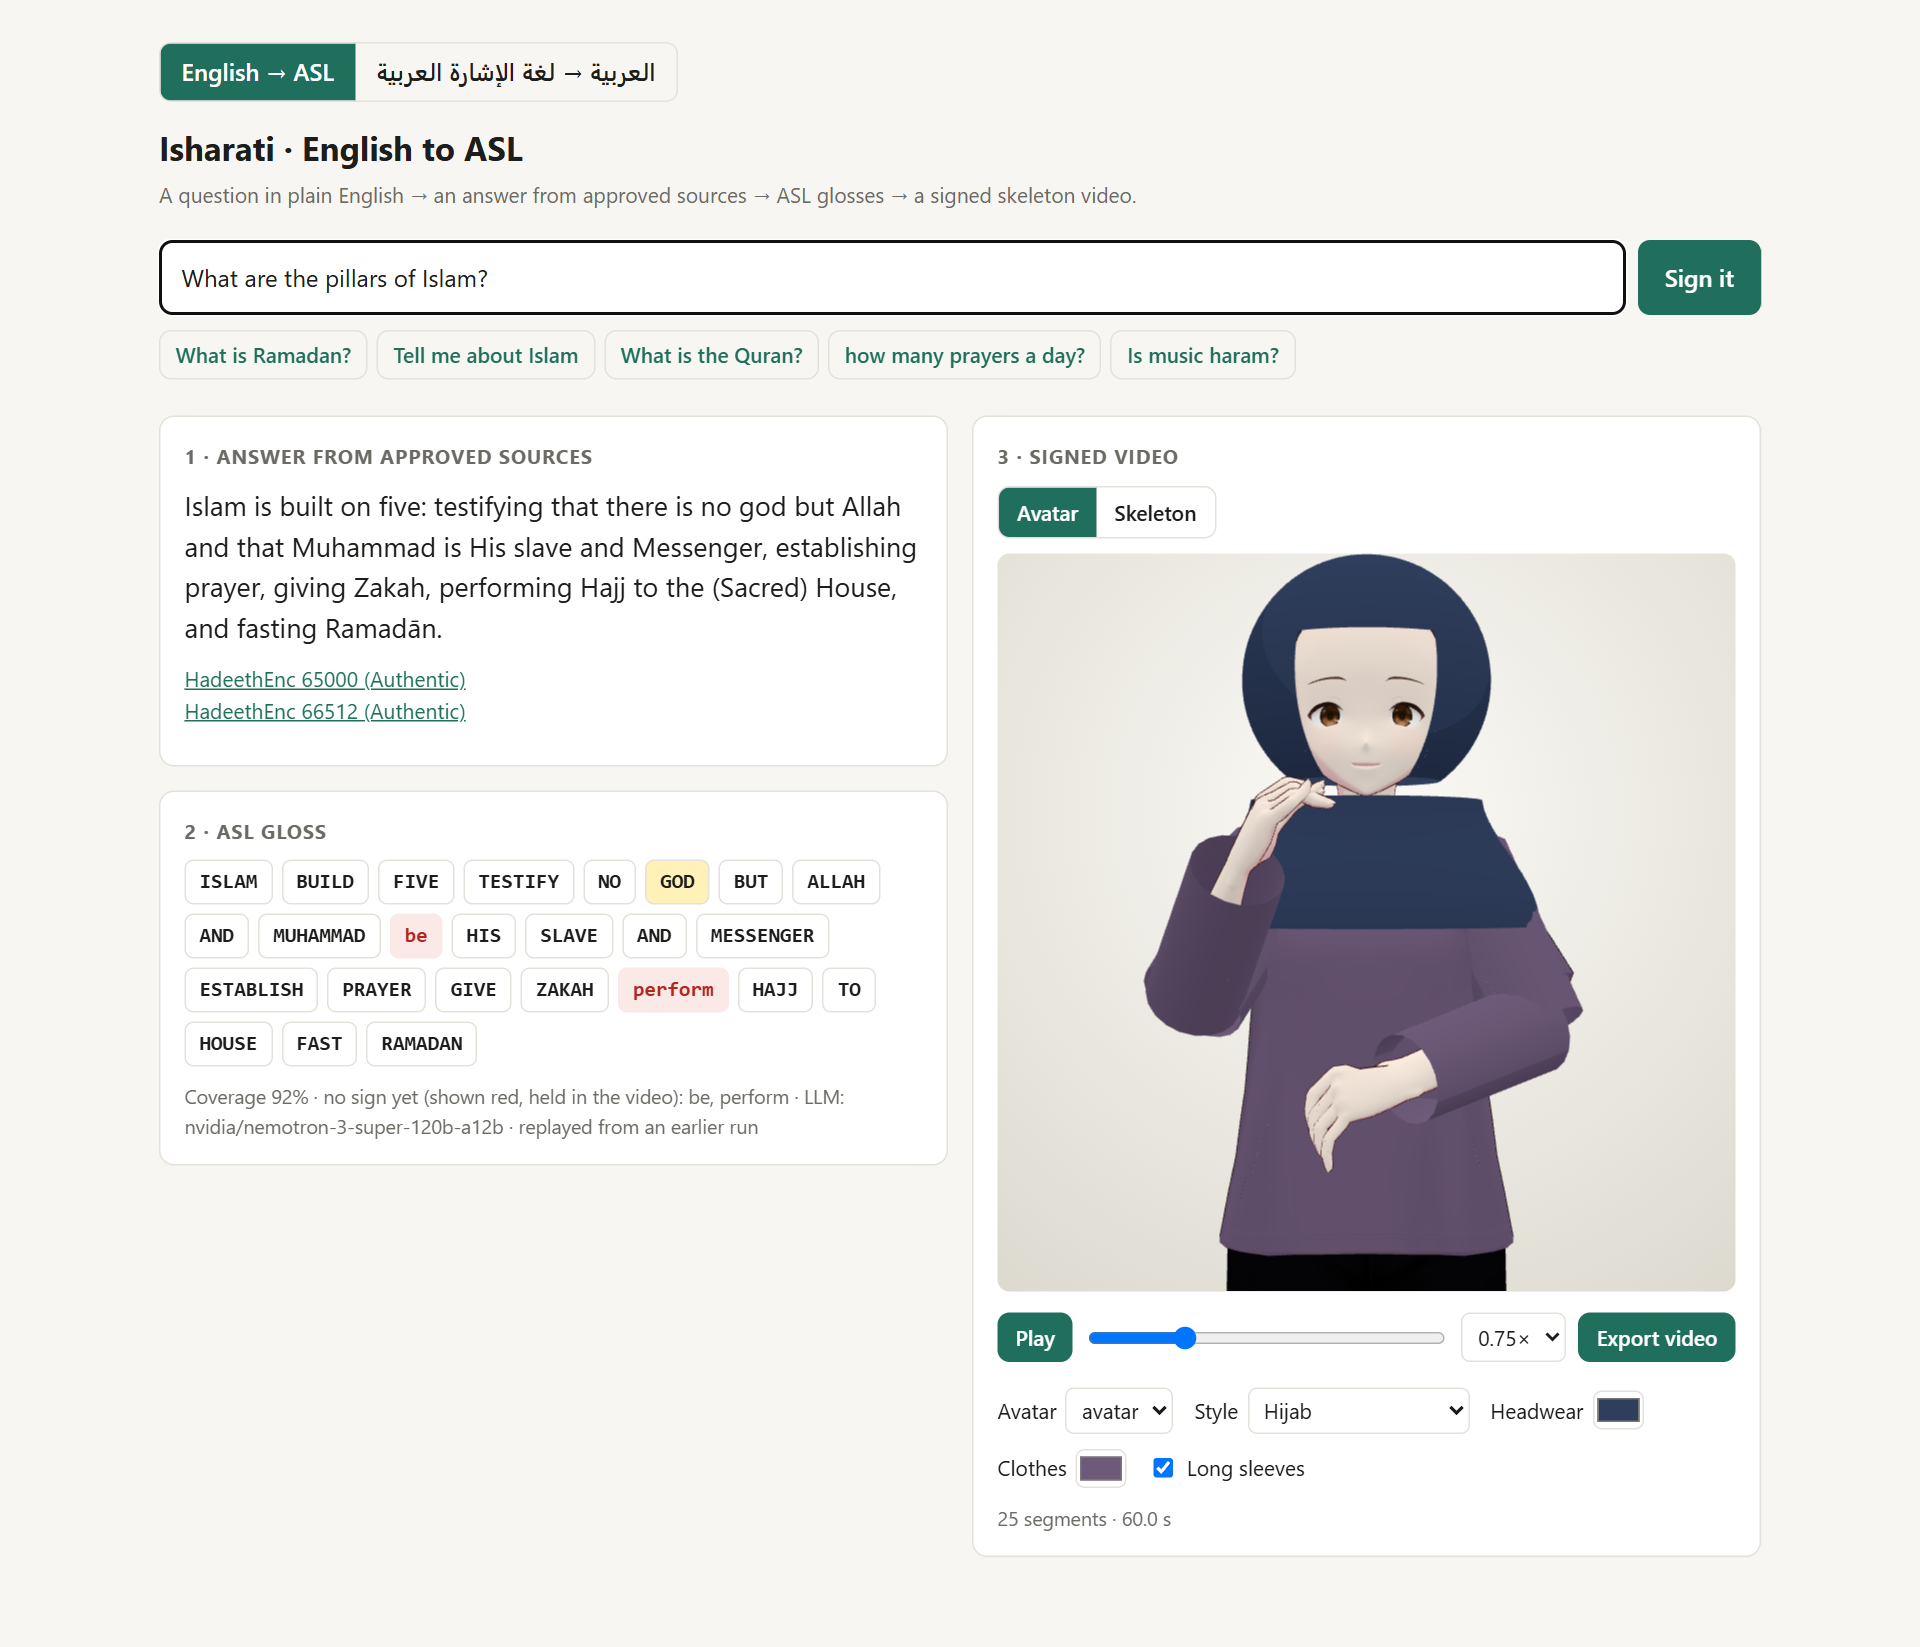
\includegraphics[width=0.49\textwidth]{figures/ui_en.png}\hfill
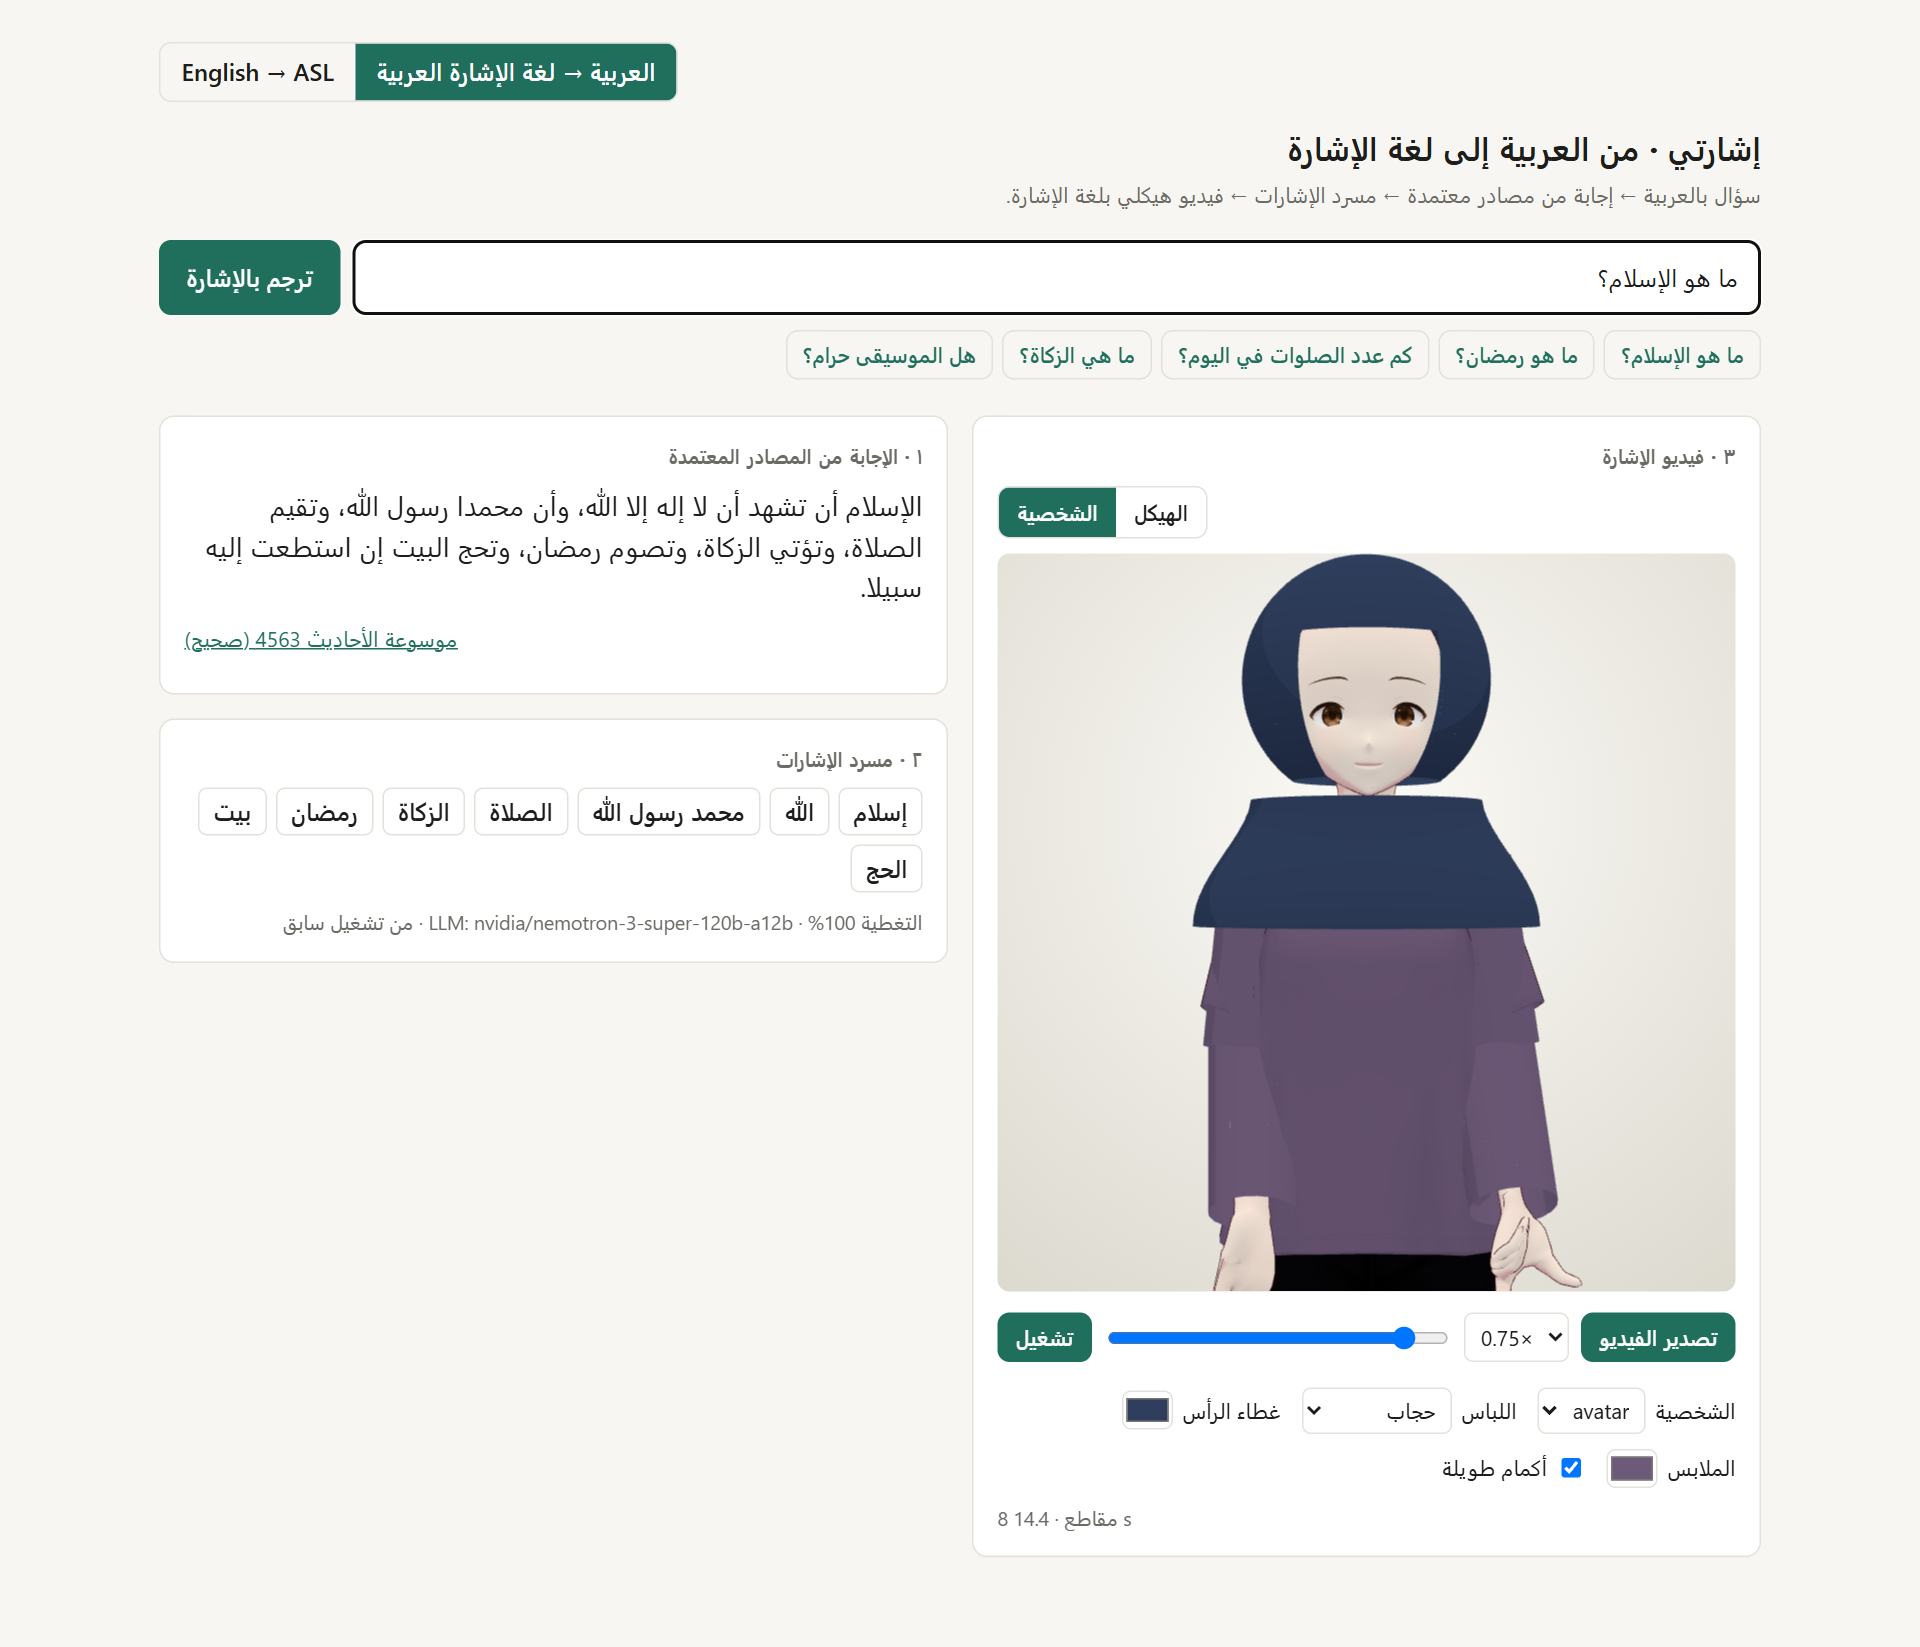
\includegraphics[width=0.49\textwidth]{figures/ui_ar.png}
\caption{The web application answering ``What are the pillars of Islam?'' in
English/ASL (left) and \ar{ما هو الإسلام؟} in Arabic/ArSL (right): grounded answer with its source links, the gloss
sequence (highlighted while signing), the avatar with the outfit panel, and the speed selector.}
\label{fig:ui}
\end{figure}

\chapter{Knowledge sources and grounded answering}
\label{sec:knowledge}

\section{Qur'an and hadith corpora}
The system answers only from two kinds of passage: Qur'an verses and hadith from HadeethEnc, the Encyclopedia of
Translated Prophetic Hadiths \cite{hadeethenc}, which publishes authenticated hadith with a grade, a title and a
scholarly explanation in many languages. Translations of the Qur'an come from QuranEnc \cite{quranenc}; the Arabic
corpus uses the Uthmani text with diacritics (linked to quran.com; see also Tanzil \cite{tanzil}).
Every passage keeps its reference and URL, which the interface shows next to the answer. Table~\ref{tab:corpora}
gives the four corpora. The hadith counts differ because HadeethEnc has not translated every hadith into every
language; every hadith in the English, Turkish and Urdu corpora also exists in the Arabic one.

\begin{table}[ht]
\centering\small
\caption{Knowledge corpora (one passage = one verse or one hadith with its title and explanation). Embeddings:
\code{intfloat/multilingual-e5-large}, 1024 dimensions, float16.}
\label{tab:corpora}
\begin{tabularx}{\textwidth}{l r r r Y Y}
\toprule
Language & Passages & Qur'an & Hadith & Qur'an text / translation & Hadith source \\
\midrule
English & 8,564 & 6,236 & 2,328 & Saheeh International (QuranEnc \code{english\_saheeh}) & HadeethEnc API, \code{en} \\
Arabic  & 9,810 & 6,236 & 3,574 & Uthmani text with diacritics (quran.com) & HadeethEnc API, \code{ar} \\
Turkish & 8,386 & 6,236 & 2,150 & Rowwad Translation Center (QuranEnc \code{turkish\_rwwad}) & HadeethEnc API, \code{tr} \\
Urdu    & 8,456 & 6,236 & 2,220 & Muhammad Junagarhi (QuranEnc \code{urdu\_junagarhi}) & HadeethEnc API, \code{ur} \\
\bottomrule
\end{tabularx}
\end{table}

The English hadith are graded \emph{authentic} (\emph{sahih}; 2,114 of 2,328) or \emph{good} (\emph{hasan}; 147), the
remainder carrying other grades as given by HadeethEnc. The source endpoints are listed in Appendix~\ref{app:urls}.

\section{Hybrid retrieval}
Each language has a BM25 index ($k_1=1.2$, $b=0.75$, hadith scores multiplied by 1.3 so that the Sunnah's explanations
are not crowded out by verse fragments) and a dense index of E5 passage embeddings (\code{passage:} and \code{query:}
prefixes, unit vectors, passages truncated to 1,500 characters). For a question $q$, the LLM adds up to 14 keywords,
giving $q'$; BM25 ranks for $q'$, the dense index for $q$ as asked, and the rankings are fused:
\begin{equation}
\mathrm{RRF}(d) = \sum_{r \in \{\mathrm{BM25},\,\mathrm{dense}\}} \frac{1}{K + \mathrm{rank}_r(d)}, \qquad K = 60.
\end{equation}
The ten best passages are passed on. If the embedding service is not running, retrieval
falls back to BM25 alone. Dense retrieval was added after lexical matching alone returned an off-topic hadith
for \ar{ما هو الإسلام؟}: the matching hadith used the words of the answer, not of the question. Hadith titles are indexed
with their text for the same reason.

\section{Grounding rules}
\label{sec:grounding}
\begin{enumerate}[leftmargin=*,itemsep=2pt]
  \item \textbf{Ruling questions are referred} before retrieval (Chapter~\ref{sec:architecture}).
  \item \textbf{Best passage first.} The LLM chooses the single passage that answers the question most directly; it
        becomes passage [1].
  \item \textbf{Answer with citations.} The LLM writes 2--4 sentences, each citing passages as [n], or replies
        \code{REFER} or \code{NO\_ANSWER}. It is told to use only the passages and to add nothing.
  \item \textbf{Support check, per sentence.} A sentence is kept only if at least 80\% of its content words
        (after normalisation and light lemmatisation) occur in the passages it cites.
        A sentence whose citations are all Qur'an verses must contain, as a contiguous run, the content-word sequence
        (stop words removed, lemmatised) of a cited verse for the text after its first colon; this stops a
        paraphrase presented as a quotation. A sentence citing a verse together with a hadith is checked only by
        the support rule. A short list of framing words (\emph{Muslims, people, also}) is exempt from the count.
        Very short replies (fewer than 6 words in English, 4 in Arabic, 5 in Turkish and Urdu) are rejected.
  \item \textbf{Drop, and rewrite if too little survives.} Unsupported sentences are dropped and listed in the
        report as dropped. If fewer than two sentences survive, the model is shown the failures
        and rewrites once. If nothing survives the status is \emph{unanswered}. (The answer prompt shows each
        passage truncated to 700 characters; the support check uses the full passage.)
\end{enumerate}
These rules came from observed failures: an early Ramadan answer added a fact absent from the cited hadith, which the
support check now removes; and bare-phrase replies are prevented by the minimum length. The cost is that some
answerable questions are declined. ``What is Ramadan?'' was unanswered in the run of 2 October 2026 because no sentence
reached the support threshold, while ``What are the pillars of Islam?'' was answered from two authentic hadith
(HadeethEnc 65000 and 66512; Figure~\ref{fig:ui}). We prefer this trade-off for religious content.

\begin{table}[ht]
\centering\small
\caption{Two runs of the live system (2 October 2026).}
\label{tab:runs}
\begin{tabularx}{\textwidth}{L{2.6cm} Y}
\toprule
Question & What are the pillars of Islam? (English $\rightarrow$ ASL) \\
Answer & Islam is built on five: testifying that there is no god but Allah and that Muhammad is His slave and
Messenger, establishing prayer, giving Zakah, performing Hajj to the (Sacred) House, and fasting Ramad\=an. \\
Glosses (23) & ISLAM BUILD FIVE TESTIFY NO GOD BUT ALLAH AND MUHAMMAD HIS SLAVE AND MESSENGER ESTABLISH PRAYER GIVE ZAKAH
HAJJ TO HOUSE FAST RAMADAN \\
Lexicon coverage & 23 of the 25 gloss items have a sign (92\%); the other two are shown as holds and reported \\
\midrule
Question & \ar{ما هو الإسلام؟} (Arabic $\rightarrow$ ArSL) \\
Answer & \ar{الإسلام أن تشهد أن لا إله إلا الله، وأن محمدا رسول الله، وتقيم الصلاة، وتؤتي الزكاة، وتصوم رمضان، وتحج البيت إن استطعت إليه سبيلا.} \\
Source & HadeethEnc 4563 (\emph{sahih}), \url{https://hadeethenc.com/ar/browse/hadith/4563} \\
Glosses (8) & \ar{إسلام} \;·\; \ar{الله} \;·\; \ar{محمد رسول الله} \;·\; \ar{الصلاة} \;·\; \ar{الزكاة} \;·\; \ar{رمضان}
\;·\; \ar{بيت} \;·\; \ar{الحج} \\
Lexicon coverage & 8 of 8 gloss items (100\%); model \code{nvidia/nemotron-3-super-120b-a12b} \\
\bottomrule
\end{tabularx}
\end{table}

\chapter{Data: sources, preprocessing and statistics}
\label{sec:lexicons}

\section{Qur'an and hadith text data}
\label{sec:textdata}
All answers come from two kinds of authoritative text, the Qur'an and the hadith. Their sources, how they are split
into passages, and the record format are described here before the sign data, because everything else (retrieval,
grounding, coverage) is defined over these passages.

\subsection{Sources}
\begin{table}[ht]
\centering\small
\caption{Sources of the Qur'an and hadith text.}
\label{tab:textsources}
\begin{tabularx}{\textwidth}{L{3.4cm} L{1.9cm} Y}
\toprule
Source & Languages & Content and use \\
\midrule
IslamicEval 2025 canonical Qur'an \cite{islamiceval} & Arabic & the 6,236 verses in Uthmani script with diacritics, one
record per verse (surah, verse number, surah name, text); the Arabic Qur'an passages \\
IslamicEval 2025 canonical hadith \cite{islamiceval} & Arabic & 34,994 records of the six canonical hadith books
(book, chapter title, text with chain of narration); kept as a reference collection, not yet indexed \\
QuranEnc translations \cite{quranenc} & English, Turkish, Urdu & Saheeh International (English), Rowwad Translation Center
(Turkish) and Muhammad Junagarhi (Urdu), one record per verse; the translated Qur'an passages \\
HadeethEnc \cite{hadeethenc} & Arabic, English, Turkish, Urdu & authenticated hadith with title, text, attribution,
grade and scholarly explanation, in parallel translations; the hadith passages of all four languages \\
\bottomrule
\end{tabularx}
\end{table}

The IslamicEval 2025 shared task on hallucination in Islamic content \cite{islamiceval} released these canonical texts
so that systems can check quoted verses and hadith against them; Isharati uses the same Qur'an text for the same purpose
(verbatim checking of verse citations, Chapter~\ref{sec:knowledge}). HadeethEnc is chosen for the hadith because every
record carries a grade and an explanation written by scholars, so an answer can quote both the hadith and its accepted
meaning, and because the same hadith is available in all four languages under one identifier.

\subsection{Signed Qur'an and Tafsir Dataset}
\label{sec:tafsirdataset}
To ground the application's vocabulary in continuous religious signing and provide direct video translations of the passages, Isharati introduces a newly curated dataset of Qur'an recitation and tafsir (exegesis) translated into Arabic Sign Language. The dataset is sourced from three major institutional efforts:
\begin{itemize}[leftmargin=*,itemsep=1pt]
  \item \textbf{King Fahd Complex for the Printing of the Holy Qur'an (\code{kfc})}: Official sign language translations of the Qur'an accompanied by tafsir, providing high-quality, authoritative interpretations.
  \item \textbf{Al-Mukhtasar fi Tafsir (\code{mukhtasar})}: A popular concise exegesis, rendered into sign language to make the meanings of the Qur'an accessible to the Deaf community.
  \item \textbf{Al-Kharj Education Department Curriculum (\code{curriculum})}: Educational videos covering selected surahs designed for Deaf students.
\end{itemize}
This dataset aligns the Arabic source text directly with the corresponding video clips of the signed performance. Furthermore, to enable 3D avatar animation and detailed linguistic analysis, the video clips are processed through Google MediaPipe Holistic to extract their skeletal keypoints (poses). The pose sequences are stored alongside the original video segments, allowing the dashboard to render both the original human performance and a stylised avatar reciting the verses or explaining the tafsir.

\subsection{From source records to passages}
\begin{itemize}[leftmargin=*,itemsep=1pt]
  \item \textbf{One verse is one passage.} Verses are short and are cited individually, so no further chunking is needed;
        the identifier is the surah and verse number (\code{q2:43}), shared by all languages.
  \item \textbf{One hadith is one passage}: its title, its text (with the narrator) and its explanation are joined, so
        that a passage answers a question on its own; the identifier is the HadeethEnc number (\code{h5907}), shared by
        all languages, and the grade is part of the reference.
  \item \textbf{Every passage keeps a reference and a link} to its source page, which the interface shows with the
        answer.
  \item \textbf{Embedding input} is the passage text truncated to 1,500 characters with the \code{passage:} prefix
        (Chapter~\ref{sec:method}); the full text is kept for the support check.
\end{itemize}
Each corpus is one JSON Lines file (one passage per line) with five fields: \code{pid} (identifier), \code{kind}
(\code{quran} or \code{hadith}), \code{reference}, \code{text} and \code{url}. Figure~\ref{fig:json} shows the source
records and the resulting passages for the same verse and the same hadith in Arabic and English.

\newcommand{\jk}[1]{\texttt{\small "#1":}}
\newcommand{\js}[1]{\texttt{\small "#1"}}
\begin{figure}[ht]
\centering\small
\fbox{\begin{minipage}{0.97\textwidth}
\textbf{(a) Source record, IslamicEval Qur'an (Arabic)}\\[2pt]
\texttt{\{}\jk{surah\_id} 1, \jk{surah\_name} \ar{"الفاتحة"}, \jk{ayah\_id} 1,\\
\hspace*{1em}\jk{ayah\_text} \ar{"بِسْمِ اللَّهِ الرَّحْمَـٰنِ الرَّحِيمِ"}\texttt{\}}\\[6pt]
\textbf{(b) Source record, HadeethEnc (fields, abridged)}\\[2pt]
\texttt{\{}\jk{id} \js{5907}, \jk{title} \js{Keep on reciting this Qur'an, ...}, \jk{hadeeth} \js{Abu Musa al-Ash`ari
reported: ...},\\
\hspace*{1em}\jk{attribution} \js{...}, \jk{grade} \js{Authentic}, \jk{explanation} \js{The Prophet ordered the Companions
...},\\
\hspace*{1em}\jk{hadeeth\_ar} \ar{"تَعَاهَدُوا هَذَا الْقُرْآنَ ..."}, \jk{grade\_ar} \ar{"صحيح"}, \jk{translations}
\texttt{["ar", "en", "tr", "ur", ...]}\texttt{\}}\\[6pt]
\textbf{(c) Passages in the English corpus}\\[2pt]
\texttt{\{}\jk{pid} \js{q1:1}, \jk{kind} \js{quran}, \jk{reference} \js{Qur'an 1:1},\\
\hspace*{1em}\jk{text} \js{In the name of Allah, the Entirely Merciful, the Especially Merciful.},\\
\hspace*{1em}\jk{url} \js{https://quranenc.com/en/browse/english\_saheeh/1\#1}\texttt{\}}\\[2pt]
\texttt{\{}\jk{pid} \js{h5907}, \jk{kind} \js{hadith}, \jk{reference} \js{HadeethEnc 5907 (Authentic)},\\
\hspace*{1em}\jk{text} \js{Keep on reciting this Qur'an ... Abu Musa al-Ash`ari reported: The Prophet said: "..."
Explanation: ...},\\
\hspace*{1em}\jk{url} \js{https://hadeethenc.com/en/browse/hadith/5907}\texttt{\}}\\[6pt]
\textbf{(d) The same passages in the Arabic corpus}\\[2pt]
\texttt{\{}\jk{pid} \js{q1:1}, \jk{kind} \js{quran}, \jk{reference} \ar{"القرآن الفاتحة 1:1"},\\
\hspace*{1em}\jk{text} \ar{"بِسْمِ اللَّهِ الرَّحْمَـٰنِ الرَّحِيمِ"}, \jk{url} \js{https://quran.com/1/1}\texttt{\}}\\[2pt]
\texttt{\{}\jk{pid} \js{h5907}, \jk{kind} \js{hadith}, \jk{reference} \ar{"موسوعة الأحاديث 5907 (صحيح)"},\\
\hspace*{1em}\jk{text} \ar{"تعاهدوا هذا القرآن ... عن أبي موسى الأشعري رضي الله عنه ... الشرح: أمر النبي ﷺ بمعاهدة القرآن ..."},\\
\hspace*{1em}\jk{url} \js{https://hadeethenc.com/ar/browse/hadith/5907}\texttt{\}}
\end{minipage}}
\caption{Record formats: (a, b) source records; (c, d) the resulting passages, one JSON object per line, for the same
verse (Qur'an 1:1) and the same hadith (HadeethEnc 5907) in English and Arabic. Identifiers are shared across languages.}
\label{fig:json}
\end{figure}

\paragraph{Size.} The four corpora hold 8,564 (English), 9,810 (Arabic), 8,386 (Turkish) and 8,456 (Urdu) passages,
each with all 6,236 verses and 2,150--3,574 hadith (Table~\ref{tab:corpora}). Hadith make up 80--89\% of the words,
because of their explanations (Chapter~\ref{sec:eda}).

\section{Preprocessing: from video to lexicon entry}
\label{sec:preproc}
Every source, whatever its form (a dictionary video per word, a lesson, a recitation in sign, a dataset of clips or a
file of precomputed keypoints), goes through the same pipeline (Figure~\ref{fig:preproc}), so that all signs end up in
one format and can be joined.

\begin{figure}[ht]
\centering
\resizebox{\textwidth}{!}{%
\begin{tikzpicture}[node distance=5mm and 5mm,
  st/.style={draw=navy, rounded corners=2pt, fill=soft, align=center, font=\footnotesize, minimum height=15mm, text width=30mm,
             inner sep=2pt},
  arr/.style={-{Stealth[length=2mm]}, thick, navy}]
  \node[st] (v) {\textbf{1. Source}\\video, lesson,\\recitation, clips};
  \node[st, right=of v] (k) {\textbf{2. Keypoints}\\MediaPipe Holistic:\\33 body, 2$\times$21 hand,\\468 face landmarks};
  \node[st, right=of k] (s) {\textbf{3. Selection}\\50 joints: 8 upper\\body + 2$\times$21 hand;\\face dropped};
  \node[st, right=of s] (n) {\textbf{4. Normalisation}\\neck origin,\\shoulder-width unit,\\25 fps, gaps filled};
  \node[st, below=9mm of n] (c) {\textbf{5. Segmentation}\\cut the sign: hand-\\visible span, captions,\\timestamps, motion};
  \node[st, left=of c] (q) {\textbf{6. Quality filter}\\reject if the hand is\\missing too often\\or the cut is too short};
  \node[st, left=of q] (m) {\textbf{7. Canonical sign}\\DTW medoid of the\\recordings; one other\\signer as template};
  \node[st, left=of m] (e) {\textbf{8. Lexicon entry}\\gloss, source, licence,\\pose, review status,\\religious flag};
  \draw[arr] (v) -- (k); \draw[arr] (k) -- (s); \draw[arr] (s) -- (n); \draw[arr] (n) -- (c);
  \draw[arr] (c) -- (q); \draw[arr] (q) -- (m); \draw[arr] (m) -- (e);
\end{tikzpicture}}
\caption{Preprocessing pipeline applied to every source. Step 5 differs per source (Table~\ref{tab:funnel}).}
\label{fig:preproc}
\end{figure}

\paragraph{Keypoints and shape.} MediaPipe Holistic \cite{mediapipe,mediapipeholistic} returns, for every video frame,
33 body landmarks, 21 landmarks for each hand and 468 face landmarks, in image coordinates with an estimated depth
(Figure~\ref{fig:mediapipe}). We
keep the 8 upper-body joints needed to place the arms (nose, neck as the mid-point of the shoulders, and both shoulders,
elbows and wrists) and all 42 hand landmarks, which carry the hand shape (Figure~\ref{fig:layout}). Each sign is
therefore a tensor of shape $[T, 50, 3]$: $T$ frames at 25 frames per second, 50 joints, and $(x, y, z)$. The face is
not kept yet; it carries the non-manual grammar of sign languages and is planned (Chapter~\ref{sec:discussion}).

\begin{figure}[ht]
\centering
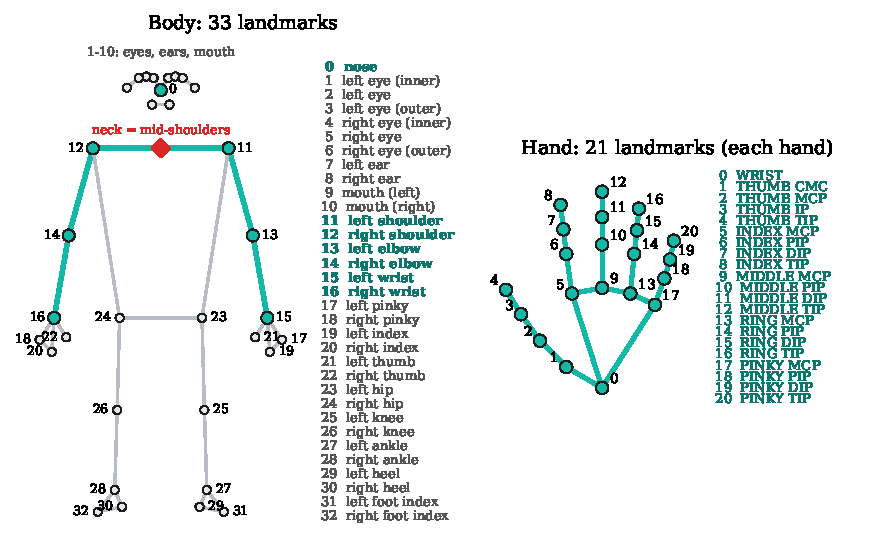
\includegraphics[width=\textwidth]{figures/mediapipe_landmarks.pdf}
\caption{MediaPipe Holistic landmarks, numbered as in its definitions (schematic, subject facing the viewer). Teal and
bold: the body landmarks Isharati keeps (nose, shoulders, elbows, wrists), plus the neck computed as the mid-point of the
shoulders (red); all 21 landmarks of each hand are kept. Grey: discarded (face detail, hand points of the body model,
hips and legs). The 468 face-mesh landmarks are not shown.}
\label{fig:mediapipe}
\end{figure}

\paragraph{Normalisation, Palm Orientation, and Glitch Elimination.}
Raw keypoints extracted across heterogeneous cameras exhibit perspective distortion, coordinate jitter, and catastrophic joint ``glitching'' during rapid wrist rotations or partial finger occlusions. To produce natural, glitch-free animations on 3D avatars and avoid kinematic artifacts, we apply a multi-stage geometric normalization pipeline:
\begin{enumerate}[leftmargin=*,itemsep=2pt]
  \item \textbf{Anthropometric Invariance:} The neck serves as the invariant spatial origin, and the clip's median shoulder width defines the unit scalar (Equation~\ref{eq:norm_pose} in Chapter~\ref{sec:method}). Frames are resampled to 25\,fps, with detection dropouts linearly interpolated.
  \item \textbf{Coordinate System Flipping and Depth Alignment:} Standard computer vision coordinates place $+Y$ downward (screen space) with arbitrary camera $Z$ scaling. We flip the vertical axis ($Y \gets -Y$) and rescale torso depth ($Z_{\text{torso}} \gets 0.5 \times Z_{\text{raw}}$) while preserving full hand dynamic depth ($Z_{\text{hands}} \gets 1.0 \times Z_{\text{raw}}$). This decouples subtle finger configurations from exaggerated torso movement.
  \item \textbf{Orthogonal Palm Frame and Normal Vector Construction:} Rather than driving 3D wrist bones via noisy raw Euler angles (which cause gimbal lock and erratic twisting), we construct an orthonormal local coordinate basis $(\mathbf{u}_{\text{palm}}, \mathbf{v}_{\text{palm}}, \mathbf{w}_{\text{palm}})$ for each hand:
  \begin{equation}
  \mathbf{u} = \frac{\mathbf{p}_{\text{mid\_mcp}} - \mathbf{p}_{\text{wrist}}}{\lVert \mathbf{p}_{\text{mid\_mcp}} - \mathbf{p}_{\text{wrist}} \rVert_2}, \quad
  \mathbf{v} = \frac{\mathbf{p}_{\text{idx\_mcp}} - \mathbf{p}_{\text{pinky\_mcp}}}{\lVert \mathbf{p}_{\text{idx\_mcp}} - \mathbf{p}_{\text{pinky\_mcp}} \rVert_2}, \quad
  \mathbf{n}_{\text{palm}} = \frac{\mathbf{u} \times \mathbf{v}}{\lVert \mathbf{u} \times \mathbf{v} \rVert_2}.
  \end{equation}
  The primary longitudinal vector $\mathbf{u}$ spans from the wrist (joint 0) to the middle knuckle (joint 9), and the transverse vector $\mathbf{v}$ connects the index knuckle (joint 5) to the pinky knuckle (joint 17). Their cross-product $\mathbf{n}_{\text{palm}}$ yields the true normal vector pointing outward from the palm.
  \item \textbf{Quaternion Hemisphere Continuity and Flip Spike Discarding:} Rotational quaternions $q$ and $-q$ represent the same physical orientation in $SO(3)$, but sudden sign flips between consecutive frames cause catastrophic 360$^\circ$ bone twists (avatar arm ``glitching''). We enforce hemisphere continuity by ensuring $\langle q_t, q_{t-1} \rangle \ge 0$; if negative, $q_t \gets -q_t$. Furthermore, if tracking loss produces an instantaneous angular jump exceeding $\Delta \theta > 2.0\,\text{rad}$ ($114.6^\circ$), the anomalous frame is discarded as an artifact spike, and the preceding stable wrist rotation is frozen and smoothed via spherical linear interpolation (SLERP, $\alpha = 0.55$).
  \item \textbf{Anatomical Clearance and Hyper-Extension Clamping:} To prevent hands from glitching backward through the 3D torso or robes, we enforce a dynamic forward clearance boundary ($Z_{\text{wrist}} \ge Z_{\text{shoulder}} + 0.38 \times L_{\text{arm}}$ whenever the hand crosses the chest midline). Individual finger segments are constrained against backward hyper-extension by projecting joint vectors onto the positive half-space defined by the palm normal $\mathbf{n}_{\text{palm}}$, clamping backward deviation to $\le -0.15 \times L_{\text{segment}}$.
  \item \textbf{Collapsed Hand Pinning:} A hand never detected in a frame (e.g., in one-handed signs or letters) is pinned cleanly to its wrist rather than collapsing to the origin, rendering as a natural resting posture rather than a stray limb.
\end{enumerate}
Figure~\ref{fig:norm} illustrates a raw video clip before and after complete normalization: signs captured from a 1080p studio camera and a 480p mobile video converge onto identical, glitch-free kinematic manifolds. Body proportions are equalized across sources at assembly time (Section~\ref{sec:render}).

\begin{figure}[ht]
\centering
\begin{minipage}{0.40\textwidth}\centering
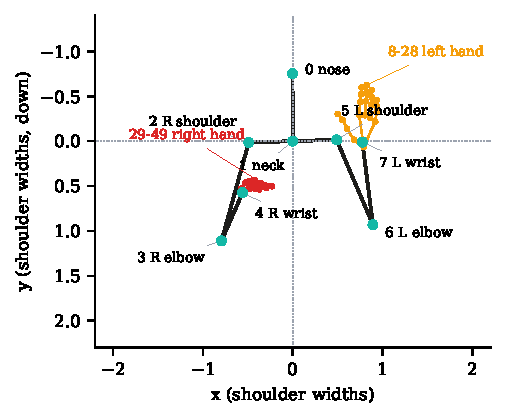
\includegraphics[width=\textwidth]{figures/keypoint_layout.pdf}
\caption{The 50 joints of the Isharati format on a real frame: 8 body joints (teal, numbered), left hand 8--28,
right hand 29--49.}
\label{fig:layout}
\end{minipage}\hfill
\begin{minipage}{0.57\textwidth}\centering
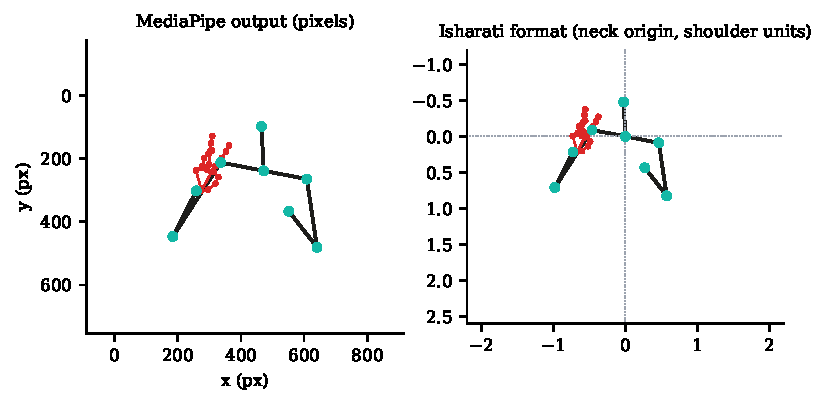
\includegraphics[width=\textwidth]{figures/normalisation.pdf}
\caption{One clip before (MediaPipe pixel coordinates) and after normalisation (neck at the origin, shoulder-width
units).}
\label{fig:norm}
\end{minipage}
\end{figure}

\paragraph{Segmentation and gloss labels.} The gloss of each sign comes from the source: the dataset label, the video
title of a one-word dictionary video, the caption of a lesson, or the word of the religious text being recited. Cutting the sign
out depends on the form of the source:
\begin{itemize}[leftmargin=*,itemsep=1pt]
  \item \textbf{One sign per video} (dictionary channels, WLASL, ASL Citizen, KArSL, T\.{I}D, CISLR, WSLP): the span in
        which a hand is raised and visible; for long clips, the first signing stretch.
  \item \textbf{Captioned lessons} (Tawasol): caption onsets and hand-raised stretches, with the term read per tile
        from contact sheets.
  \item \textbf{Explained dictionaries} (Saudi dictionary): the first motion segment after a coloured label.
  \item \textbf{Qur'an recitation in sign} (Al-Kharj curriculum): the interpreter signs in time with a recitation;
        Whisper word timestamps aligned to the Qur'an text give each word's frames, and the medoid over occurrences of a
        lemma becomes the sign.
  \item \textbf{Continuous narrative and scripture} (Deaf Bible EGCBT): segmented automatically using our continuous
        RoPE Transformer pose segmentation model, followed by monotonic verse-constrained gloss alignment.
  \item \textbf{Islamic term lists} (GDM, Noor): signing stretches anchored by Whisper timestamps of the spoken term.
  \item \textbf{One-word Shorts} (Levantine): the most recurring 0.5--2.5\,s motion segment.
  \item \textbf{Continuous sentence corpora} (ArabSign, Isharah, How2Sign, YouTube-ASL): preserved as continuous utterance sequences for translation and recognition benchmarks, while serving as rich sources for sign mining (e.g., weakly supervised multiple-instance learning on YouTube-ASL and How2Sign to mine individual signs for lexicon gaps, or continuous boundary modeling with our RoPE Transformer), rather than raw unsegmented dictionary entries.
\end{itemize}

\subsection{Continuous Stream Processing with RoPE Transformer Segmentation}
Continuous sign language poses lack discrete audio boundaries when recordings are deaf-first or silent (such as the Deaf Bible EGCBT recordings, where audio tracks register below $-91\,\text{dB}$). In accordance with the system methodology defined in Section~\ref{sec:rope_segmentation}, we apply our pre-trained Rotary Position Embedding (RoPE) Transformer segmentation model~\cite{signsegmentation}\footnote{Sign language pose segmentation repository: \url{https://github.com/sign-language-processing/segmentation}} to partition continuous pose streams into discrete word-level signs without speech alignment.

As formulated in Equation~\eqref{eq:velocity} and Equation~\eqref{eq:rope}, the model operates directly on normalized 3D joint positions and inter-frame velocities ($50 \times 6 = 300$ dimensions), utilizing 4 Transformer encoder layers with RoPE self-attention to label every frame UNK, O, B or I, at about 290 frames per second on a desktop CPU (Section~\ref{sec:results_segmentation}) using the pre-trained \code{model.safetensors} weights (11.5\,MB)\footnote{Pre-trained RoPE Transformer model checkpoint release: \url{https://github.com/sign-language-processing/segmentation/releases/tag/v0.1.0}}. A sign opens at \texttt{B}, continues through \texttt{I}, and closes at \texttt{O} or \texttt{UNK}; spans shorter than 4 frames are rejected. Our benchmark (Section~\ref{sec:results_segmentation}) shows that these boundaries are not yet reliable, in particular when the pose is normalised as in our wrapper rather than as in the package.

\paragraph{Verse-Constrained Monotonic Gloss Alignment.}
Once continuous pose sequences are segmented into millisecond-accurate physical sign boundaries, we align individual gesture segments to Arabic lexical glosses using verse-constrained monotonic dynamic matching. For narrative corpora with parallel text (such as Deaf Bible EGCBT with 47 canonical Scripture stories)\footnote{Deaf Bible Society Egyptian Sign Language chronological catalog: \url{https://deafbible.com/EGCBT}}, the text of each chapter is tokenized into Arabic lemmas. Because sign order in Egyptian Sign Language (ESL) predominantly mirrors chronological narrative order with topic-comment shifts, segment boundaries are mapped monotonically to the ordered set of content words $\{w_1, w_2, \dots, w_K\}$, matching physical duration against lexical syllabic weight. Signs identified with high confidence provide anchor points, establishing ground-truth aligned continuous sign datasets.

\paragraph{Quality filter and canonical sign.} A recording is rejected when the dominant hand is missing in too many
frames (more than 30\% for ASL Citizen, 45\% for the dictionary channels) or the cut is shorter than six frames. Where
several recordings of a gloss exist, the DTW medoid becomes the canonical sign, and a recording by a different signer is
kept as a back-translation template. The entry records the gloss, its aliases, the source, the pose, whether it is a
religious term or a letter, and its review status. Table~\ref{tab:funnel} follows each source from raw material to
the merged lexicons; the merge keeps one sign per gloss, preferring Islamic sources and Deaf-signer dictionaries.

\begin{table}[ht]
\centering\small
\caption{From raw material to lexicon: what each source provided, what was extracted, and how many glosses it
contributes to the merged lexicons (after duplicates are resolved in favour of earlier sources).}
\label{tab:funnel}
\begin{tabularx}{\textwidth}{L{3.6cm} Y r r}
\toprule
Source & Raw material $\rightarrow$ extraction & Signs extracted & Glosses in lexicon \\
\midrule
\multicolumn{4}{l}{\emph{ASL (English mode)}} \\
GDM Islamic signs & 1 video, 40 terms, Whisper-anchored & 41 & 75 \\
Noor For Sign & 1 Ramadan lesson & 7 & 14 \\
Obscure ASL & one-word videos & 102 & 96 \\
ASL Citizen & 83,399 clips of 2,731 glosses; medoid of 3 signers, + 2,259 templates & 2,626 & 2,204 \\
WLASL & 679 glosses not yet covered, up to 2 clips each & 1,241 & 666 \\
\midrule
\multicolumn{4}{l}{\emph{ArSL (Arabic mode)}} \\
KArSL-502 & 4,016 clips, 502 signs, 3 signers; medoid & 502 & 512 \\
Qur'an curriculum & 22 surahs signed with recitation; Whisper--Qur'an alignment & 353 & 332 \\
Tawasol & 154 lesson videos; caption-based cuts & 336 & 205 \\
Saudi / Arabic dictionary explained & 17 videos; label-triggered cuts & 105 & 84 \\
Dictionary channels (unified, Kuwaiti, children's, scouts') & 6,698 one-word clips; 2,137 rejected by the filter & 4,559 & 2,694 \\
Levantine Shorts & 133 videos; recurring-motion cut & 131 & 152 \\
\midrule
\multicolumn{4}{l}{\emph{T\.{I}D (Turkish mode) and ISL (Urdu mode)}} \\
T\.{I}D S\"ozl\"u\u{g}\"u & 5,017 one-word clips (extraction in progress) & 1,308 & 1,374 \\
CISLR & 4,765 words, one reference clip each & 3,965 & 3,965 \\
WSLP 2025 & word-recognition training set & 4,056 & 4,020 \\
\midrule
\multicolumn{4}{l}{\emph{Sentence data (not cut into lexicon signs)}} \\
ArabSign & 6 signers $\times$ 50 sentences, $\sim$30 repetitions & 9,259 sentence poses & -- \\
YouTube-ASL & 391,494 captioned clips (10 parts) & 39,052 (part 1) & -- \\
\bottomrule
\end{tabularx}
\end{table}

\section{The YouTube-ASL keypoint dataset}
\label{sec:ytasl}
YouTube-ASL \cite{youtubeasl} pairs 391,494 sentence clips from 9,422 YouTube videos with their English captions; its
keypoint release \cite{youtubeaslkp} provides, for every clip, MediaPipe landmarks per frame (33 body, 21 per hand, 478
face, in pixels) as one JSON file, 374\,GB in ten archives. We convert it to the Isharati format in the cloud, one
archive at a time so that no local disk is needed: body and hand joints are selected, the face is dropped, coordinates
are normalised, and each archive becomes one compressed array file of clips (about 40$\times$ smaller: 37.5\,GB to
0.91\,GB for the first part) plus a manifest. The manifest has one row per clip: clip and video identifiers, start and
end frame in the source video, number of frames, frame size, the share of frames in which each hand is detected, and the
archive part; the English sentence and the train/dev split are joined from the captions. The result is published as a
Hugging Face dataset with the CC BY 4.0 attribution of the source (Figure~\ref{fig:hf}).

\begin{figure}[ht]
\centering
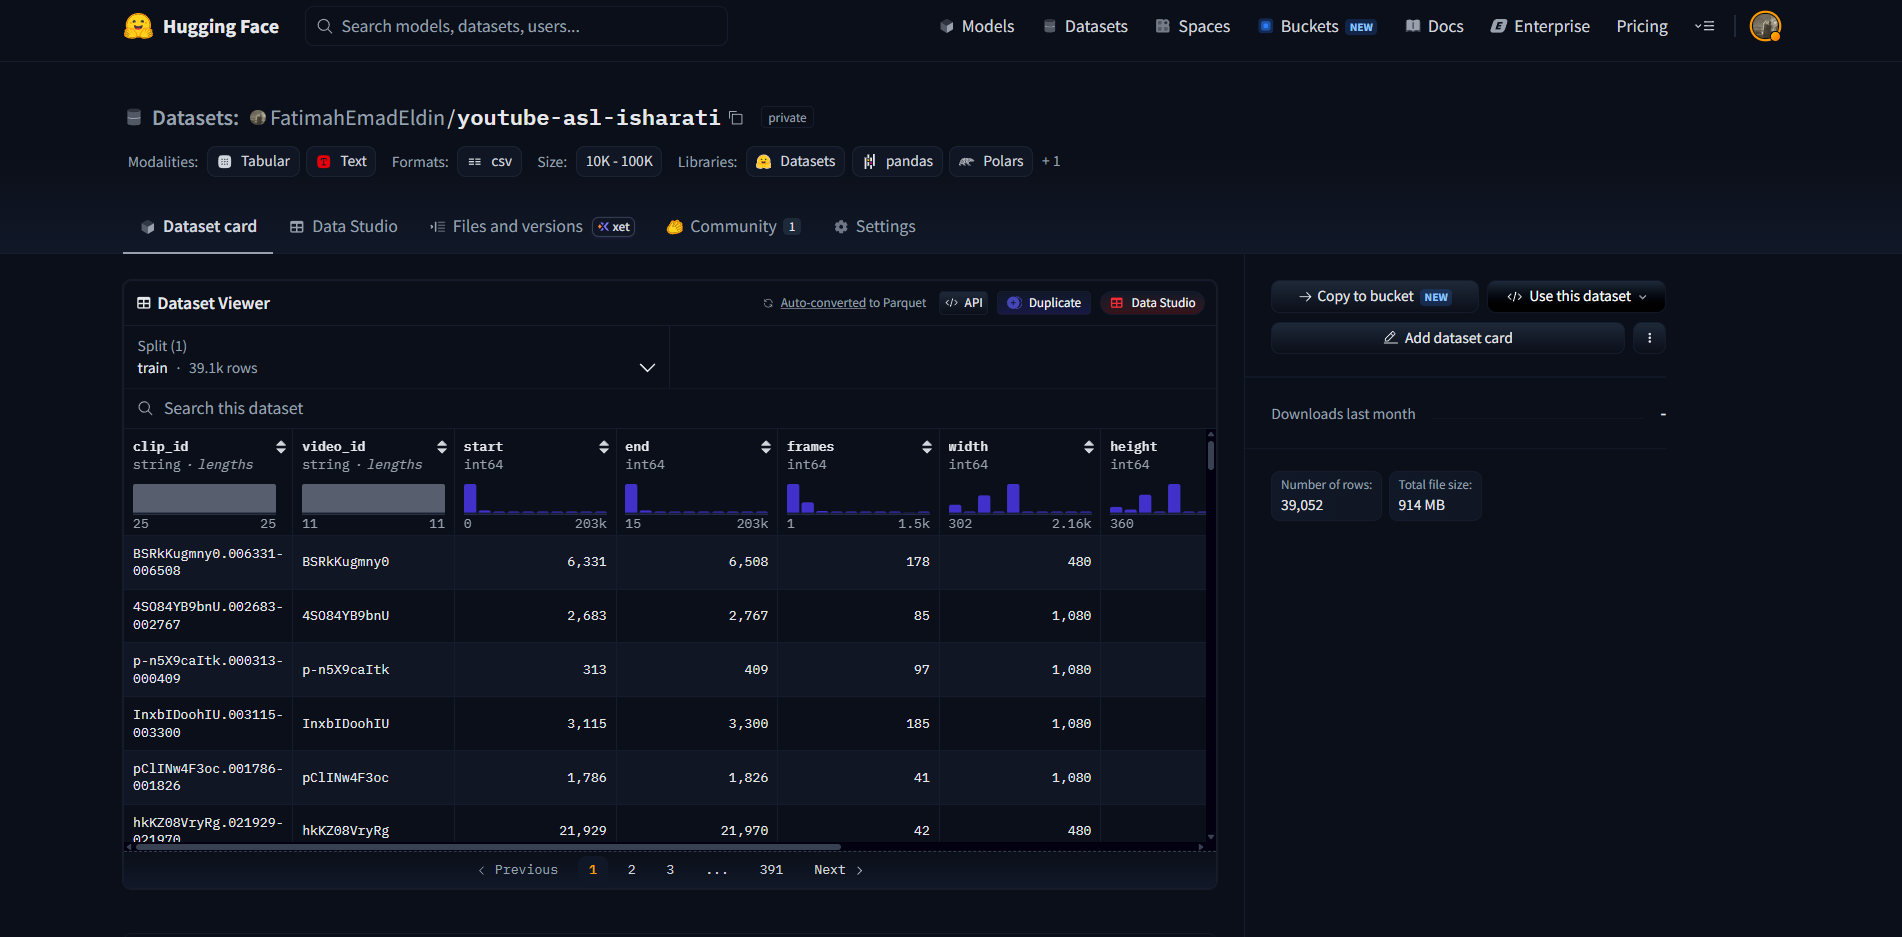
\includegraphics[width=\textwidth]{figures/hf_dataset.png}
\caption{The converted YouTube-ASL dataset on Hugging Face (first part: 39,052 clips, one manifest row per clip).}
\label{fig:hf}
\end{figure}

The first part holds 39,052 clips from 7,818 videos; 99.7\% are matched to their English sentence. Clips last a median
of 107 frames (about 3.6\,s; 5th--95th percentile 36--300), and 96\% have a hand detected in at least half of their
frames (Figure~\ref{fig:ytstats}); recordings range from 1080p webcams to 480p phones. These clips are used to train the
weakly supervised sign spotter of Chapter~\ref{sec:results}; 407 of the 500 most frequent uncovered Qur'an and hadith
words occur in the captions of this part alone.

\begin{figure}[ht]
\centering
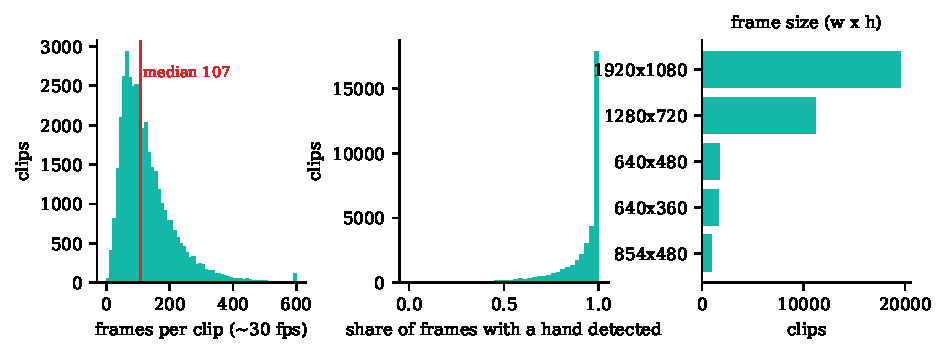
\includegraphics[width=\textwidth]{figures/youtube_asl_stats.pdf}
\caption{The first converted part of YouTube-ASL: clip length (red: median), share of frames with a hand detected, and
the most common frame sizes.}
\label{fig:ytstats}
\end{figure}


\section{English mode: American Sign Language}
\begin{table}[ht]
\centering\small
\caption{ASL lexicon: 3,491 glosses over 3,288 sign recordings, 99 of
them religious. When two sources have the same gloss, the first source in the table wins (Islamic sources first).}
\label{tab:asl}
\begin{tabularx}{\textwidth}{L{3.2cm} r L{3.5cm} L{3.0cm} Y}
\toprule
Source & Glosses & Covers & Licence & Reference / Link \\
\midrule
GDM 40 Islamic signs\footnotemark & 75 & Islamic terms, one Deaf signer (aliases: 40 $\rightarrow$ 75) & not stated (public video) & YouTube \code{L-lWEt7OeJk} \\
Noor For Sign, Ramadan\footnotemark & 14 & Ramadan vocabulary & not stated (public video) & YouTube \code{VWzAH0j56f4} \\
Obscure ASL channel\footnotemark & 96 & general, one word per video & owner permission needed & YouTube channel \\
ASL Citizen~\cite{aslcitizen}\footnotemark & 2,204 & general dictionary (2,731 glosses, 83,399 clips) & Microsoft Research licence & NeurIPS 2023 \\
WLASL v0.3~\cite{wlasl}\footnotemark & 666 & general (2,000 glosses); missing fetched & C-UDA, research use & WACV 2020 / GitHub \\
YouTube-ASL~\cite{youtubeasl}\footnotemark & 436 & general vocabulary from educational videos & YouTube Standard / CC BY & NeurIPS 2023 \\
MS-ASL~\cite{msasl}\footnotemark & 0 & queued: $\sim$140 words absent from both & C-UDA, research use & BMVC 2019 \\
\midrule
\textbf{Total} & \textbf{3,491} & & & \\
\bottomrule
\end{tabularx}
\end{table}
\addtocounter{footnote}{-7}%
\stepcounter{footnote}\footnotetext{GDM 40 Islamic signs video: \url{https://www.youtube.com/watch?v=L-lWEt7OeJk}}%
\stepcounter{footnote}\footnotetext{Noor For Sign Ramadan lesson: \url{https://www.youtube.com/watch?v=VWzAH0j56f4}}%
\stepcounter{footnote}\footnotetext{Obscure ASL channel: \url{https://www.youtube.com/@obscureasl}}%
\stepcounter{footnote}\footnotetext{ASL Citizen dataset: \url{https://www.microsoft.com/en-us/research/project/asl-citizen/}}%
\stepcounter{footnote}\footnotetext{WLASL GitHub repository: \url{https://github.com/dxli94/WLASL}}%
\stepcounter{footnote}\footnotetext{YouTube-ASL repository: \url{https://github.com/google-research/google-research/tree/master/youtube_asl}}%
\stepcounter{footnote}\footnotetext{MS-ASL dataset: \url{https://www.microsoft.com/en-us/research/project/ms-asl/}}%

\paragraph{Sentence-level ASL data.} How2Sign \cite{how2sign} (31,165 training sentences; MediaPipe Holistic
features, still packed) and YouTube-ASL (Section~\ref{sec:ytasl}) serve two purposes: training the back-translation
recogniser, and mining single signs for the Qur'an and hadith words the lexicon lacks. No sentence-level sign is in
the lexicon yet.

\section{Arabic mode: Arabic Sign Language}

\subsection{Arabic Signed Qur'an and Tafsir Datasets}
To properly represent Islamic texts in Arabic Sign Language (ArSL), we specifically targeted official and curriculum-based signed Qur'an and Tafsir datasets. General ArSL dictionaries are insufficient for the domain-specific vocabulary and stylistic recitation required for Qur'anic texts. We collected and processed three primary sources of continuous signed recitation and explanation (Tafsir):
\begin{itemize}
    \item \textbf{King Fahd Complex for the Printing of the Holy Qur'an:}\footnote{King Fahd Complex official portal and signed interpretations: \url{https://qurancomplex.gov.sa/}} The official, authoritative signed explanations of the Qur'an produced by the Complex. These high-quality video clips provide the baseline for theological accuracy in sign.
    \item \textbf{Al-Mukhtasar fi Tafsir (Abridged Tafsir):}\footnote{Al-Mukhtasar fi Tafsir sign language broadcasts: \url{https://www.youtube.com/@tafsir_center}} A simplified yet comprehensive signed translation of the Qur'an's meanings, mapping the verses into clear, accessible ArSL.
    \item \textbf{Al-Kharj Education Department Curriculum:}\footnote{Al-Kharj Education Department Qur'an recitation in sign playlist: \url{https://www.youtube.com/channel/UCRpE_0EQWEJhf_8WCW6hxKg}} Educational signed recitations covering every Qur'anic lemma of 22 short Surahs, designed for educational environments.
\end{itemize}
The video clips from these three datasets were aligned with their Arabic transcriptions and processed through MediaPipe to extract continuous 3D skeletal keypoints. These sequences are embedded directly into the Qur'an recitation dashboard, allowing the 3D avatars to perform official, verified signed recitations for users.

\begin{figure}[ht]
\centering
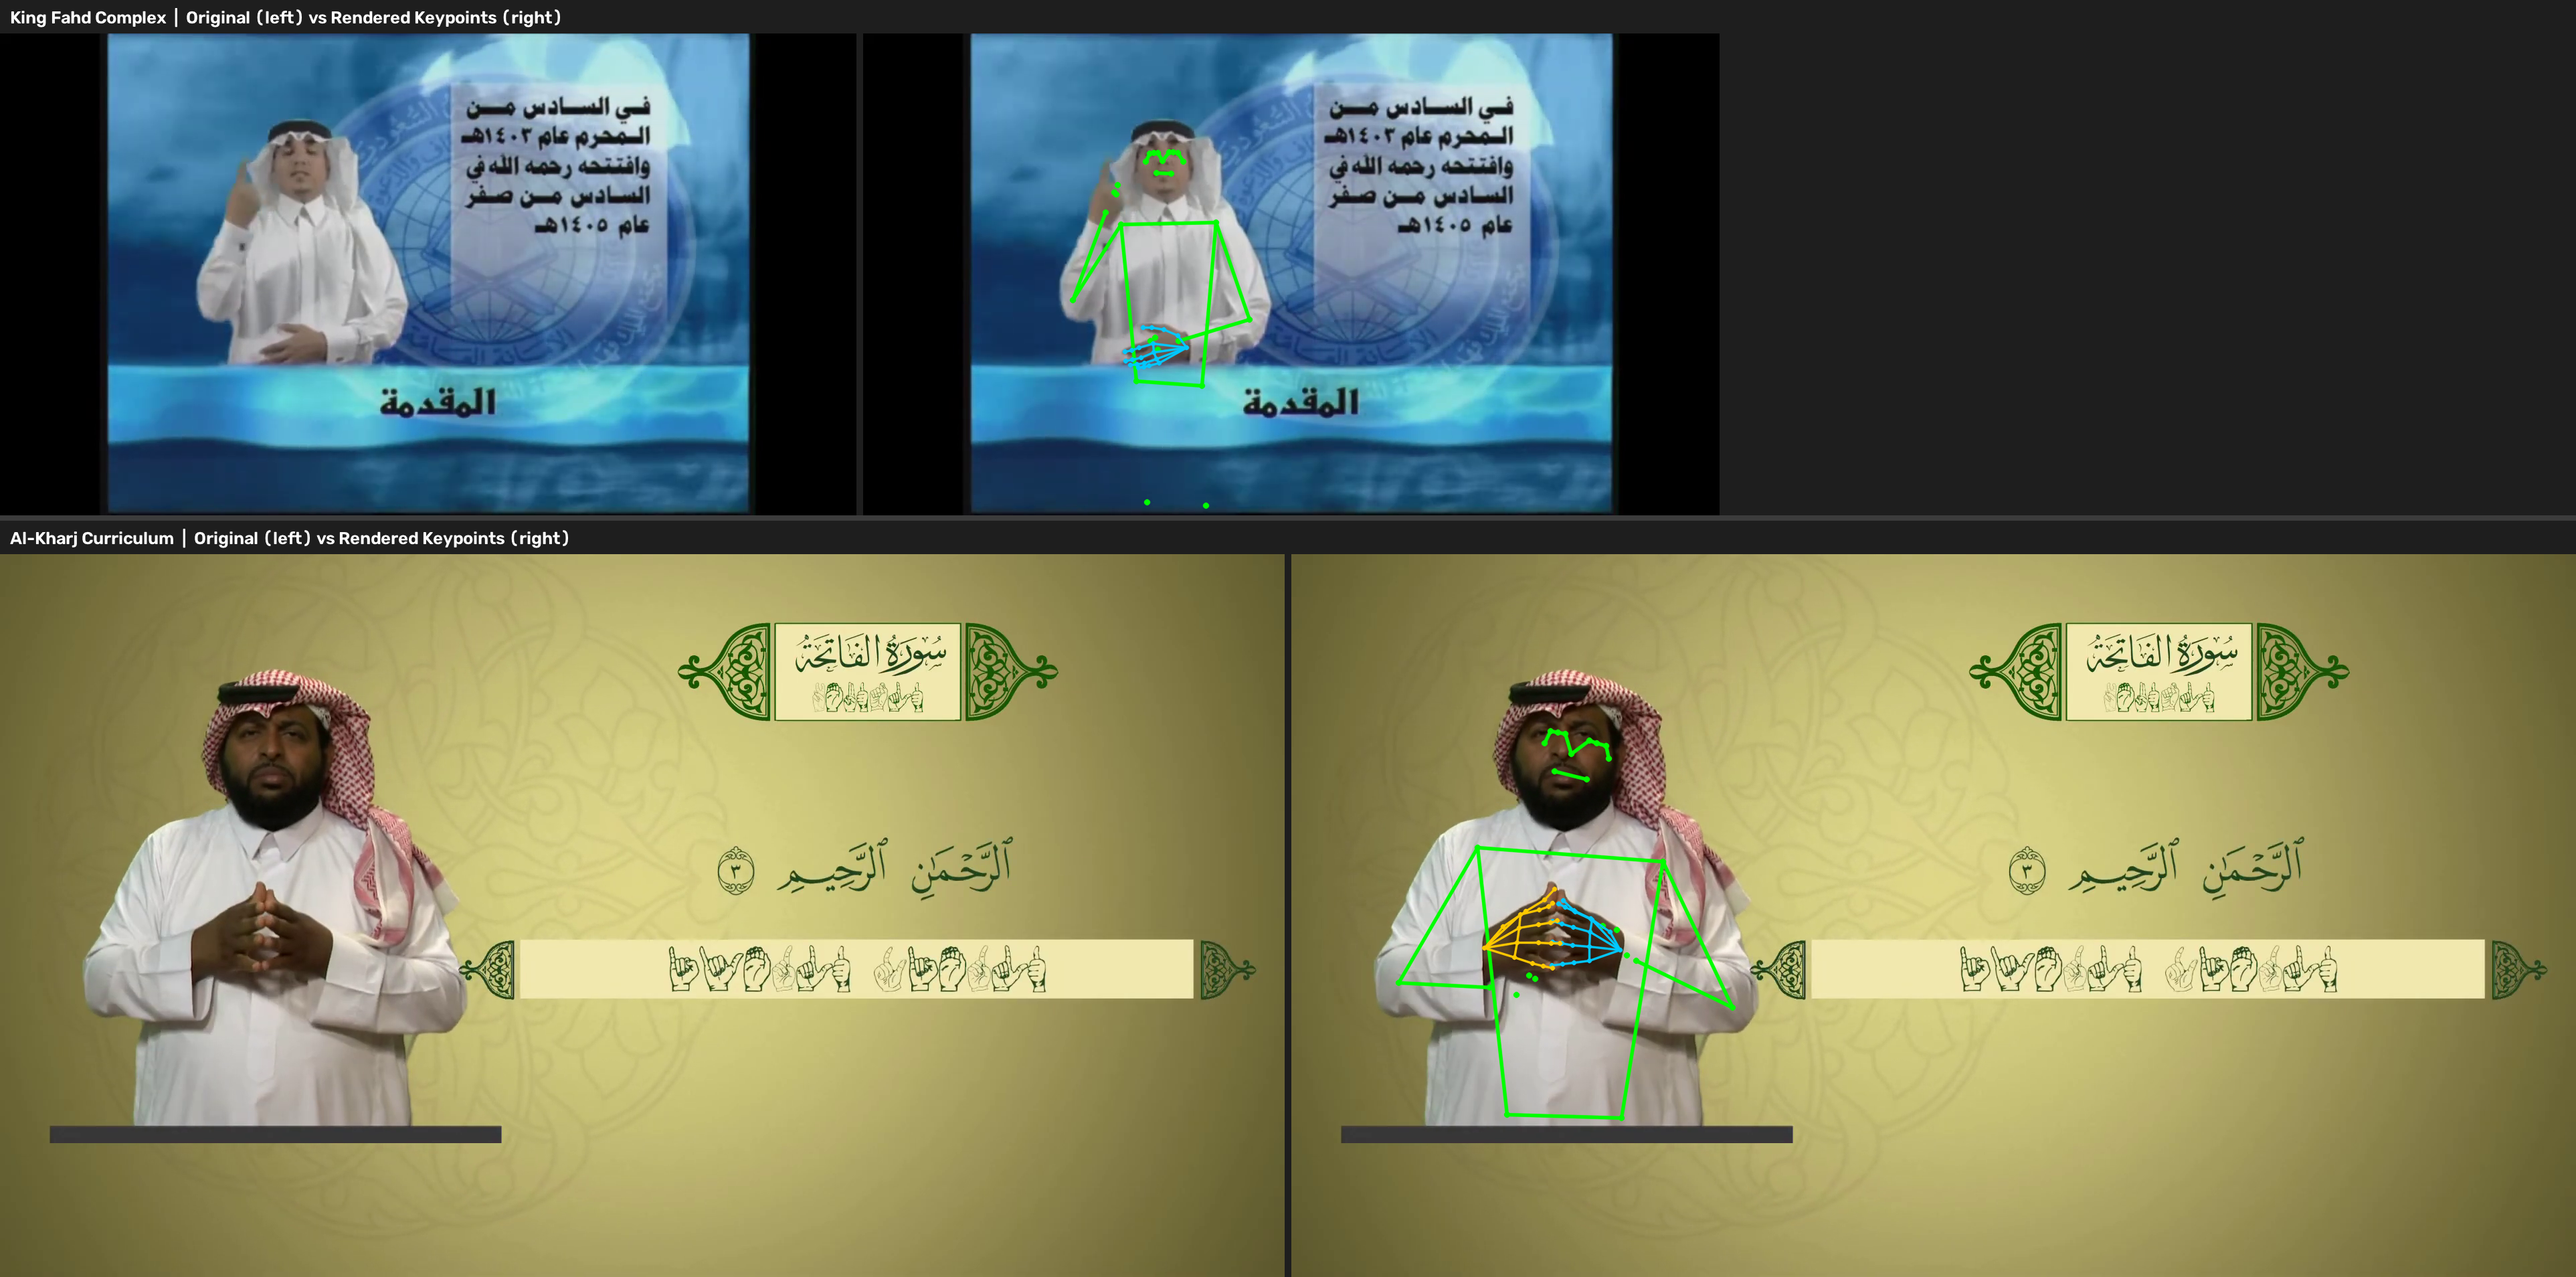
\includegraphics[width=\textwidth,height=0.4\textheight,keepaspectratio]{figures/tafsir_datasets_composite.png}
\caption{Actual frames extracted from the saved YouTube videos of signers performing Qur'anic recitation and Tafsir. \textbf{Top:} King Fahd Complex official signed explanation (``Al-Muqaddimah''), with original frame (left) and rendered MediaPipe keypoints overlay (right) showing body pose (green), left hand (yellow), and right hand (cyan). \textbf{Bottom:} Al-Kharj curriculum recitation of Surah Al-Fatiha, verse 3 (``Al-Rahman Al-Rahim''), with the same keypoint extraction pipeline applied.}
\label{fig:tafsir_sample}
\end{figure}

\subsection{ArSL Lexicon Composition and Source Breakdown}
\begin{table}[ht]
\centering\small
\caption{Comprehensive ArSL lexicon: 6,610 verified glosses across 11 unified datasets (2,941 religious terms), categorized by extraction modality: \textbf{3,551 Isolated Dictionary signs} vs. \textbf{3,059 Continuous Segmented signs}. Duplicates resolved hierarchically with priority to authentic Islamic recitations and deaf-first sources.}
\label{tab:arsl}
\begin{tabularx}{\textwidth}{L{3.2cm} r L{2.2cm} L{3.0cm} L{1.8cm} Y}
\toprule
Source & Glosses & Modality Type & Domain / Coverage & Licence & Reference / Link \\
\midrule
New Arabic Sources (Broadcasts)\footnotemark & 2,409 & Continuous & 20 religious and educational channels, ASR-aligned & not stated & YouTube (249 videos) \\
Unified Arabic Sign Dictionary~\cite{arslunified}\footnotemark & 1,424 & Isolated & Pan-Arab standardized dictionary ($\sim$2,700 clips) & not stated & Official dictionary \\
Kuwaiti Sign Dictionary\footnotemark & 978 & Isolated & Gulf and Kuwaiti dialect sign vocabulary & not stated & Official dictionary \\
KArSL-502 / Extended~\cite{karsl}\footnotemark & 840 & Isolated & Isolated Saudi signs, 3 native signers & research use & Kaggle / KAU \\
Qur'an Curriculum, Al-Kharj\footnotemark & 305 & Continuous & 22 short Surahs, word-by-word recitation & not stated & YouTube channel \\
Tawasol Center\footnotemark & 196 & Continuous & Islamic pillars, calendar, conversational signs & not stated & YouTube (153 videos) \\
Levantine Shorts (Jordan/Palestine)\footnotemark & 149 & Continuous & Conversational Levant sign vocabulary & not stated & YouTube playlist \\
Scouts' Sign Dictionary\footnotemark & 140 & Isolated & Arab Scouting and civil vocabulary & not stated & Official dictionary \\
Children's Sign Dictionary\footnotemark & 87 & Isolated & Specialized pediatric and educational signs & not stated & Official dictionary \\
Arabic Dictionary (Explained)\footnotemark & 43 & Isolated & Morphological and linguistic sign analysis & not stated & YouTube channel \\
Saudi Dictionary (Explained)\footnotemark & 39 & Isolated & Saudi linguistic terms and colloquial glosses & not stated & YouTube channel \\
\midrule
\textbf{Total Master Lexicon} & \textbf{6,610} & \multicolumn{4}{l}{\textbf{3,551 Isolated Signs} · \textbf{3,059 Continuous Segmented Signs} · 2,941 Religious} \\
\bottomrule
\end{tabularx}
\end{table}
\addtocounter{footnote}{-11}%
\stepcounter{footnote}\footnotetext{New Arabic Sources video corpus: 249 videos across 20 curated Arabic deaf instruction channels.}%
\stepcounter{footnote}\footnotetext{Unified Arabic sign dictionary: \url{https://www.youtube.com/channel/UCg85d6jX2GANVz1msIvFvnA}}%
\stepcounter{footnote}\footnotetext{Kuwaiti sign dictionary: \url{https://www.youtube.com/channel/UCiILcu4Zyk_j4L8tEe2UmVQ}}%
\stepcounter{footnote}\footnotetext{KArSL dataset on Kaggle: \url{https://www.kaggle.com/datasets/yousefdotpy/karsl-502}}%
\stepcounter{footnote}\footnotetext{Al-Kharj Qur'an channel: \url{https://www.youtube.com/channel/UCRpE_0EQWEJhf_8WCW6hxKg}}%
\stepcounter{footnote}\footnotetext{Tawasol Center sign language channel: \url{https://www.youtube.com/@tawasol9282}}%
\stepcounter{footnote}\footnotetext{Levantine Shorts playlist: \url{https://www.youtube.com/playlist?list=PLqZ7C4R4F6EJOnp0lRkKSM9RswCr6WBSG}}%
\stepcounter{footnote}\footnotetext{Scouts' sign dictionary: \url{https://www.youtube.com/channel/UCiILcu4Zyk_j4L8tEe2UmVQ}}%
\stepcounter{footnote}\footnotetext{Children's sign dictionary: \url{https://www.youtube.com/channel/UCiILcu4Zyk_j4L8tEe2UmVQ}}%
\stepcounter{footnote}\footnotetext{Arabic sign dictionary explained: \url{https://www.youtube.com/channel/UCQiTnBVnBfvVYilcfjpKkMA}}%
\stepcounter{footnote}\footnotetext{Saudi sign dictionary explained: \url{https://www.youtube.com/channel/UCQiTnBVnBfvVYilcfjpKkMA}}%

\paragraph{Breakdown of Continuous Broadcast Sources (\texttt{new\_arabic\_sources}).}
The largest single collection in our unified repository originates from the continuous digitization and automated segmentation of 249 long-form broadcast videos across 20 distinct thematic playlists. Table~\ref{tab:new_sources_categories} details the specific distribution of content across Islamic pedagogy, legal rulings, prophetic biography (\emph{Seerah}), Qur'anic exegesis (\emph{Tafsir}), and linguistic lessons.

\begin{table}[ht]
\centering\small
\caption{Thematic category breakdown of the 249 broadcast video sources in \code{new\_arabic\_sources}, totaling 483,571 MediaPipe Holistic pose frames and 2,409 unique religious and conversational glosses.}
\label{tab:new_sources_categories}
\begin{tabularx}{\textwidth}{L{4.2cm} r L{5.8cm}}
\toprule
Thematic Playlist / Category & Videos & Content Scope and Religious Focus \\
\midrule
\code{teacher\_of\_deaf} & 57 & Comprehensive sign pedagogy, school curricula, moral values \\
\code{sawt\_al\_anamil} & 37 & Islamic daily supplications, Eid takbeerat, family life \\
\code{hussein\_al\_owrtani} & 27 & Islamic principles, jurisprudence, practical Islamic etiquette \\
\code{aljazeera\_al\_ishara\_lughati} & 23 & Fasting rulings, Ramadan virtues, Islamic geographical names \\
\code{cda\_dubai\_words} & 21 & Dubai Community Development Authority official civic signs \\
\code{ishara\_curated\_playlist} & 17 & Curated religious lessons and general deaf educational discourse \\
\code{dawah\_deaf\_mahabbat\_al\_nabi} & 13 & Love of the Prophet \ar{ﷺ}, sunnah practices, devotional sign \\
\code{naji\_zakarneh\_seerah} & 13 & Prophetic biography episodes signed by Sheikh Naji Zakarneh \\
\code{dawah\_deaf\_hayah\_saeedah} & 12 & Marital happiness, family jurisprudence, marital communication \\
\code{naji\_zakarneh\_tafsir\_amma} & 6 & Word-by-word signed exegesis of Juz' Amma (Surahs 78--114) \\
\code{naji\_zakarneh\_deen} & 5 & Pillars of faith, Islamic Creed (\emph{Aqeedah}), Hajj rituals \\
\code{asasiyat\_lughat\_al\_ishara} & 4 & Fundamentals of Arabic Sign Language and religious formulas \\
\code{dawah\_deaf\_khutbahs} & 4 & Official Friday and Arafah sermons from the Two Holy Mosques \\
\code{naji\_zakarneh\_signs} & 3 & Essential theological signs explained in Jordan dialect \\
\code{dawah\_deaf\_dawrah\_ilmiyyah\_14} & 2 & Intensive scholarly seminar on Islamic jurisprudence \\
\code{dawah\_deaf\_adab\_islamiyyah} & 1 & Explanation of Islamic manners (\emph{Kitab al-Adab}) \\
\code{dawah\_deaf\_fusool\_seerah} & 1 & Chapters in the biography of the Messenger \ar{ﷺ} \\
\code{deen\_wa\_ma\_yataalaq\_bihi} & 1 & Monotheism and essential religious requirements \\
\code{aljazeera\_religious} & 1 & Professional studio broadcast on Islamic sign communication \\
\code{osama\_tahrawi\_jordan} & 1 & Specialized Jordanian conversational and religious signs \\
\midrule
\textbf{Total Broadcast Sources} & \textbf{249} & \textbf{483,571 Frames} · \textbf{2,409 Unique Glosses} \\
\bottomrule
\end{tabularx}
\end{table}

\begin{figure}[ht]
\centering
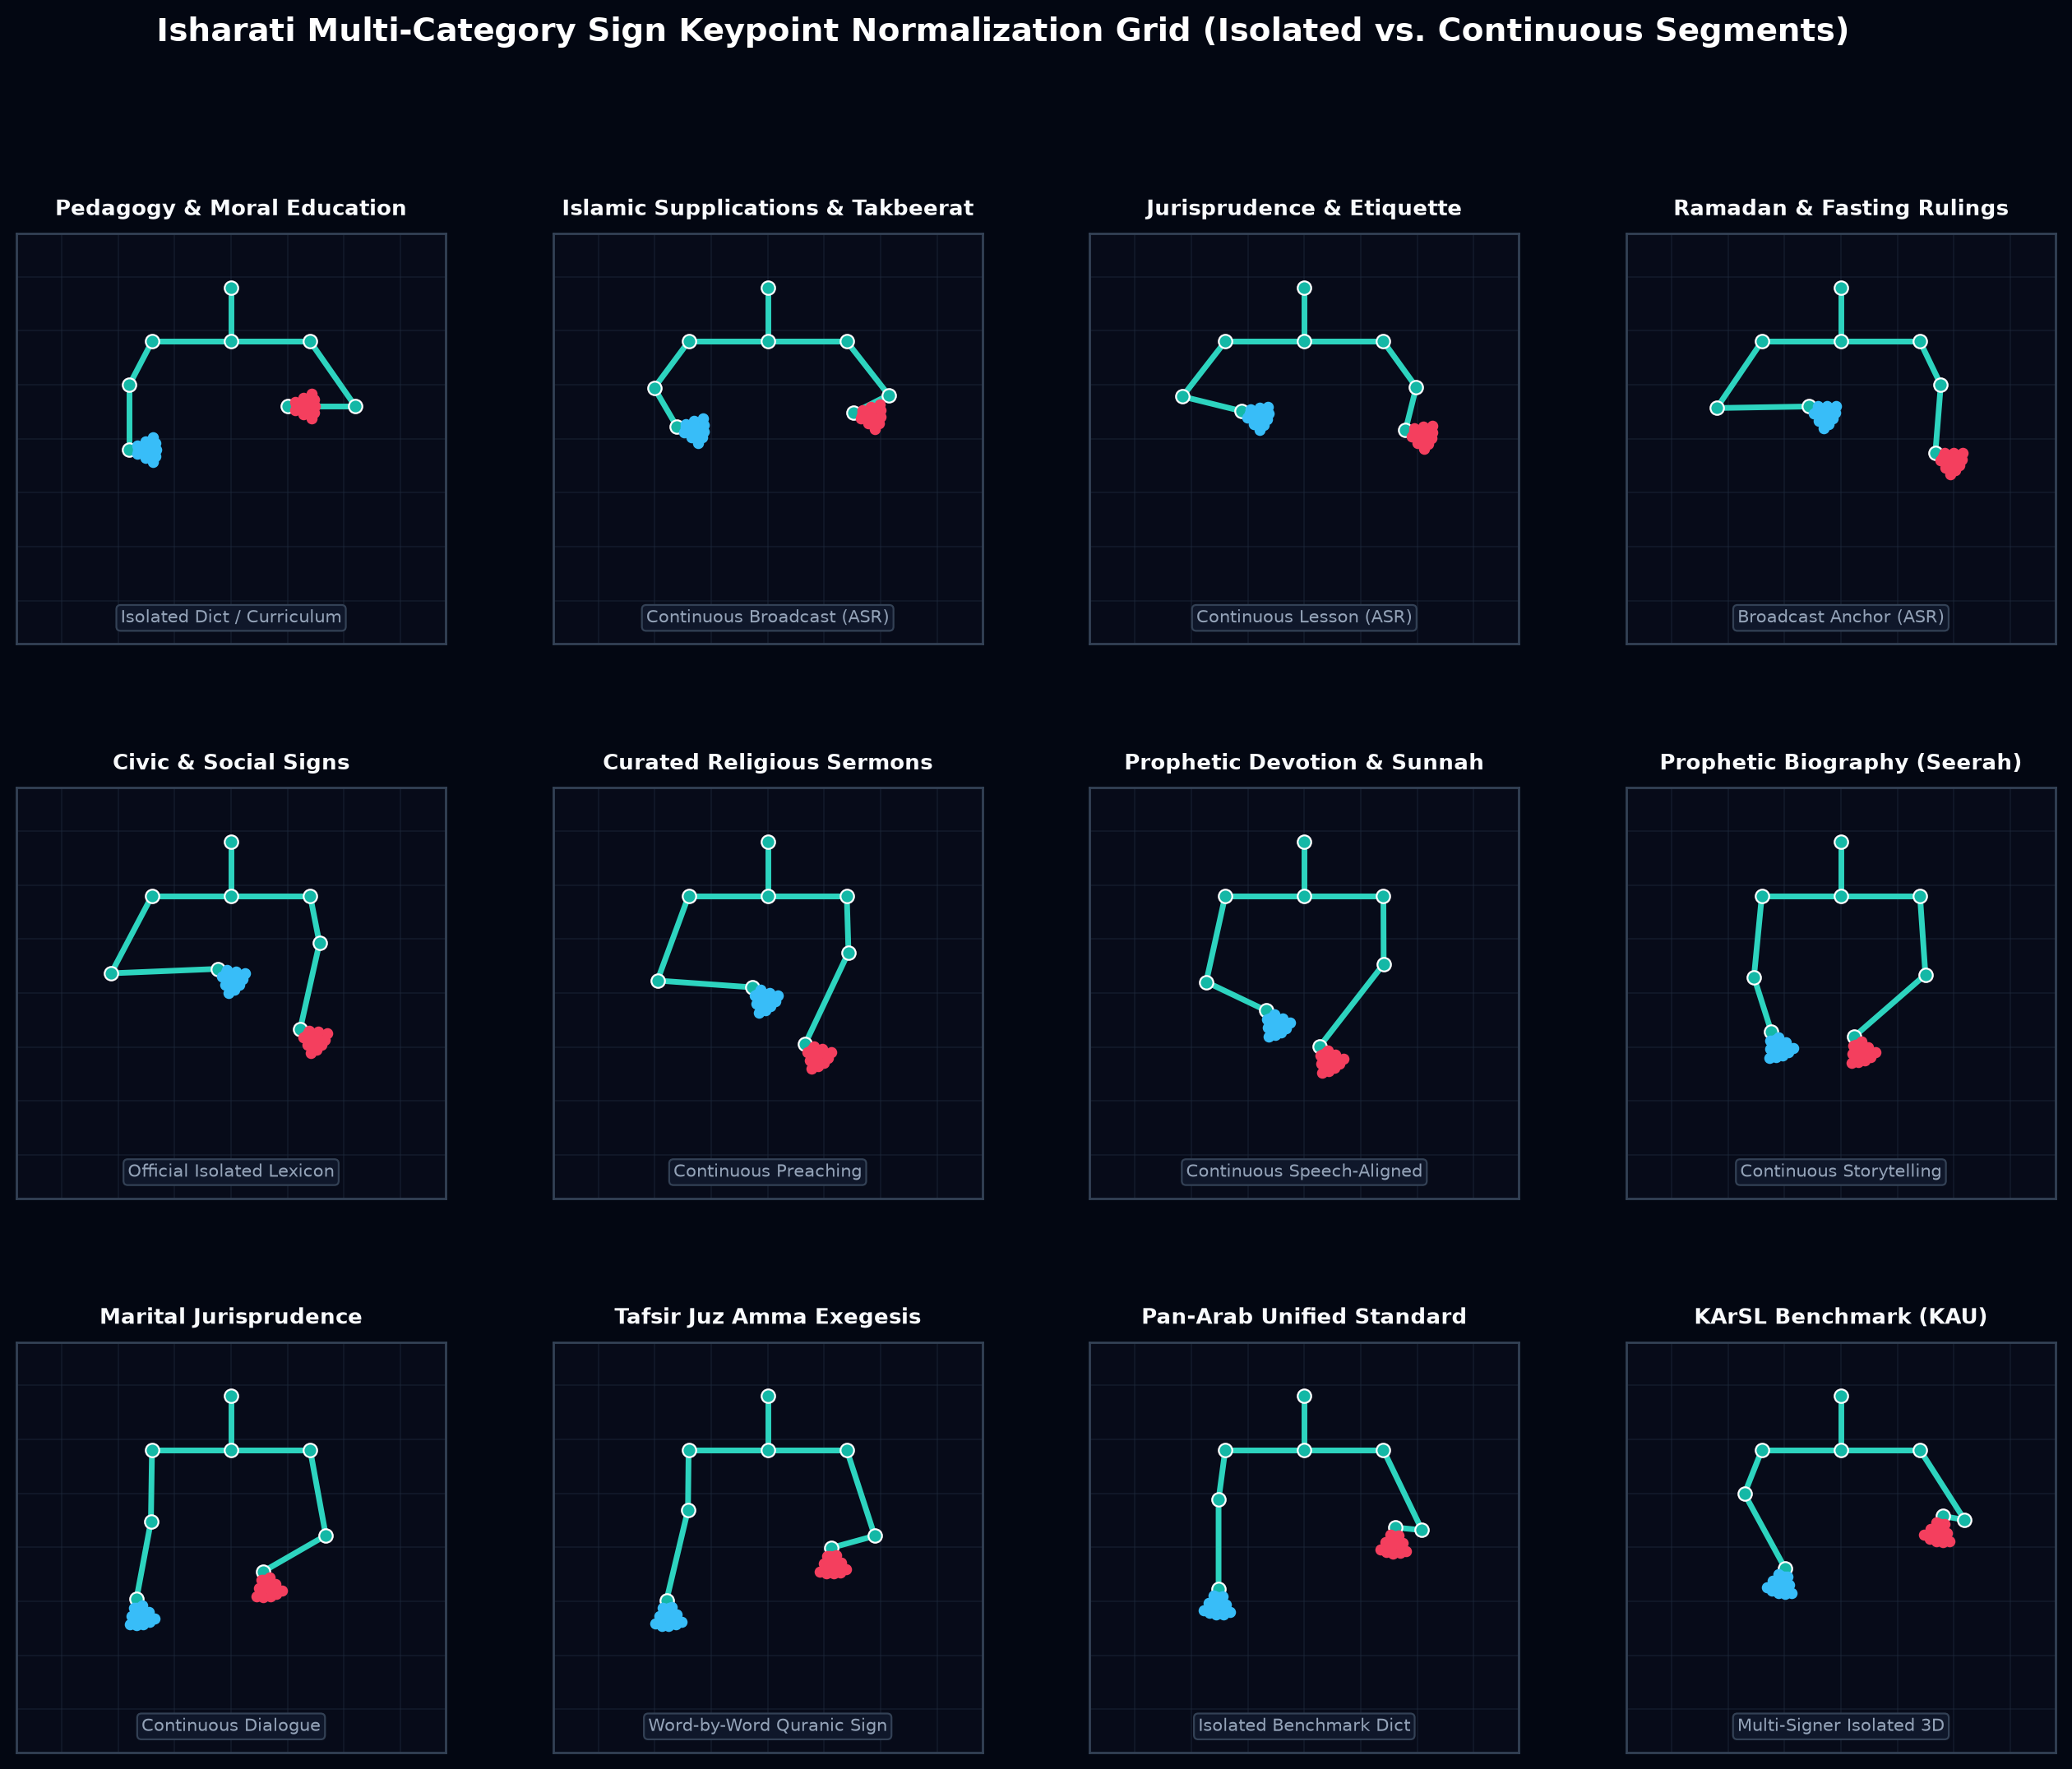
\includegraphics[width=\textwidth]{figures/category_normalization_grid.png}
\caption{\textbf{Multi-category sign keypoint normalization and continuous segmentation grid.} Representative standardized $[T, 50, 3]$ skeletal frames across 12 distinct Arabic sign sources, comparing isolated dictionary benchmarks (e.g., KArSL-502, Unified Arabic Dictionary, CDA Dubai) with continuous ASR-aligned and RoPE-segmented broadcast categories (e.g., Al-Jazeera Ramadan rulings, Sawt Al-Anamil supplications, Hussein Al-Owrtani jurisprudence, Naji Zakarneh Seerah and Juz' Amma exegesis). Each frame depicts normalized upper-body bones (teal), right-hand 21-joint articulated kinematic chains (crimson), and left-hand articulated chains (sky blue) mapped against the centered holographic coordinate basis.}
\label{fig:category_grid}
\end{figure}

\paragraph{Arabic sentence data and ArabSign benchmark.} 
The ArabSign dataset~\cite{arabsign} comprises continuous Arabic Sign Language sequences recorded with Microsoft Kinect V2 depth sensors across 6 native Deaf signers performing 51 distinct sentences in multi-sentence sessions (9,259 total video clips: 7,426 train and 1,833 test; median length 95 frames)\footnote{ArabSign official repository and benchmark: \url{https://github.com/Hamzah-Luqman/ArabSign}}. The dataset covers daily conversation, medical instructions, and essential Islamic formulas (\ar{الحمد لله}, \ar{السلام عليكم}, \ar{يوم القيامة}, \ar{خطبة الجمعة}, \ar{الصلاة الخمس}). 

Because ArabSign provides continuous, multi-sign sentence utterances rather than isolated signs, we investigated automated segmentation to isolate individual lexical signs. However, frame-level CTC alignments and attention weights from the baseline Seq2Seq Encoder-Decoder model (which utilizes an attention-augmented recurrent decoder achieving $W\!E\!R \approx 13.9\%$)\footnote{ArabSign Seq2Seq with Bahdanau attention model: \url{https://github.com/Hamzah-Luqman/ArabSign/tree/main/ArabSign-EncoderDec}} yielded diffuse soft attention distributions rather than strict physical sign boundaries. We therefore maintain ArabSign in its native continuous sentence structure for continuous sign recognition evaluation and text-to-gloss validation (Chapter~\ref{sec:evaluation}), while employing our pre-trained RoPE Transformer segmentation model (Section~\ref{sec:rope_segmentation}) to demarcate physical gesture boundaries across continuous sessions. The pretrained baseline weights from the ArabSign benchmark provide a canonical comparative reference for our sequence modeling experiments.

\paragraph{SignBank+ Multilingual Dataset Integration.}
To expand lexical coverage across Arabic and international sign systems, we integrate SignBank+ \cite{signbankplus}\footnote{SignBank+ multilingual sign language repository: \url{https://github.com/sign-language-processing/signbank-plus}}. SignBank+ compiles community-contributed SignWriting representations cleaned and expanded via large language models. By parsing parallel lexical pairings and SignWriting-to-spoken language tables, SignBank+ contributes 6,035 validated Arabic gloss candidates and cross-lingual translation mappings that bootstrap our text-to-gloss canonical lemma index.

\paragraph{Deaf Bible EGCBT Corpus Digitization.}
To extend our continuous ArSL corpus with high-resolution narrative data, we reverse-engineered and digitized the Egyptian Sign Language Chronological Bible Translation (EGCBT) corpus from the Deaf Bible Society~\cite{deafbible_egcbt}\footnote{Deaf Bible Society EGCBT portal: \url{https://deafbible.com/EGCBT}}. The corpus encompasses 47 chronological biblical narrative stories recorded in 1080p high definition by Deaf Egyptian signers. Because the audio tracks are silent placeholders ($-91\,\text{dB}$), speech-to-text alignment is inapplicable. We processed all episodes through our MediaPipe Holistic extraction and RoPE Transformer continuous segmentation pipeline, generating standardized $[T, 50, 3]$ skeletal trajectories, `.pose` files, and `.npz` arrays. Using our verse-constrained monotonic alignment, the physical sign segments are grounded directly into Arabic narrative glosses, yielding an open-source digital corpus of continuous Egyptian Sign Language. \emph{Caveat:} this segmentation used the same faulty label decoder as the Isharah mining described below, so these segments must be regenerated with the fixed decoder before they are used.

\paragraph{Isharah corpus: an attempted re-segmentation, withdrawn.}
The Isharah dataset~\cite{isharah} comprises 21,450 continuous Saudi Sign Language sentences recorded by native Deaf
signers, covering 1,090 distinct glosses. Heuristic pauses and CTC alignment gave inconsistent cuts (same/different-gloss
DTW ratio 0.926, close to random). We then mined word clips with the RoPE Transformer segmenter
(Section~\ref{sec:rope_segmentation}), which produced 1,113 candidate glosses. An audit before merging showed that these clips
are not usable, and they are \textbf{not} in the lexicon:
\begin{itemize}[leftmargin=*,itemsep=2pt]
  \item the wrapper that decoded the model's frame labels used the wrong label indices (the package defines UNK\,=\,0,
    O\,=\,1, B\,=\,2, I\,=\,3; the wrapper treated 1 and 2 as signing), so it marked the gaps between signs rather than the
    signs. The mined ``single signs'' last 4--6.7\,s (\ar{أنا} 5.6\,s, \ar{هو} 4.4\,s), several times a typical sign;
  \item the stored clips were in raw frame coordinates with missing joints set to zero, not in the $[T,50,3]$
    normalised contract, and 73 clips were shared by two or more unrelated glosses;
  \item their ``approved'' status had been set automatically from occurrence counts, not by review.
\end{itemize}
The decoder has been fixed. Isharah will be re-mined with it and vetted (single-sign duration, consistency of the same
gloss across signers, agreement with existing dictionary signs) before anything is added. Because Isharah covers
many everyday words, a correct re-mining could add real coverage.

\section{Arabic normalisation and coverage audit}
\label{sec:ar_norm}

\paragraph{Where the uncovered words are.} Coverage is the share of all content-word occurrences in the Qur'an and hadith
corpus (591,448 after stopwords) that the matcher links to a sign; it is not the share of our glosses. To see why 42.9\,\% are
uncovered, every uncovered word type was analysed with CAMeL Tools (part of speech, lemma, root) and assigned to the first
matching reason (Table~\ref{tab:ar_missing}, Figure~\ref{fig:ar_missing}). Only 4.8\,\% of occurrences are words we have no
sign for; most of the rest are words we \emph{do} sign, written in a form the matcher did not recognise.

\begin{table}[ht]
\centering\small
\caption{Why Arabic content words were uncovered (share of all content-word occurrences, before the fixes below).}
\label{tab:ar_missing}
\begin{tabularx}{\textwidth}{L{6.2cm} r Y}
\toprule
Reason & Share & Examples \\
\midrule
Verb form; its lemma has a sign & 12.3\,\% & \ar{قالت، يكون، قالوا، كانوا، قلت} $\to$ \ar{قال، كان} \\
Same root as a sign, different word (needs review) & 11.3\,\% & \ar{قبل، رواية، قوله، الصحابة} \\
Function word missing from the stopword list & 6.5\,\% & \ar{عنه، إلا، ولا، به، أنه، منه} \\
Noun/adjective form; its lemma has a sign & 4.1\,\% & \ar{ربك، ربنا، يده، بيده} $\to$ \ar{رب، يد} \\
Proper name & 3.8\,\% & \ar{عباس، عمرو، مسعود، جبريل} \\
Truly missing: noun/adjective & 2.9\,\% & \ar{الدنيا، سبيل، عذاب، الإبل} \\
Truly missing: verb & 1.9\,\% & \ar{أخذ، حصل، ينبغي} \\
\bottomrule
\end{tabularx}
\end{table}

\begin{figure}[ht]
\centering
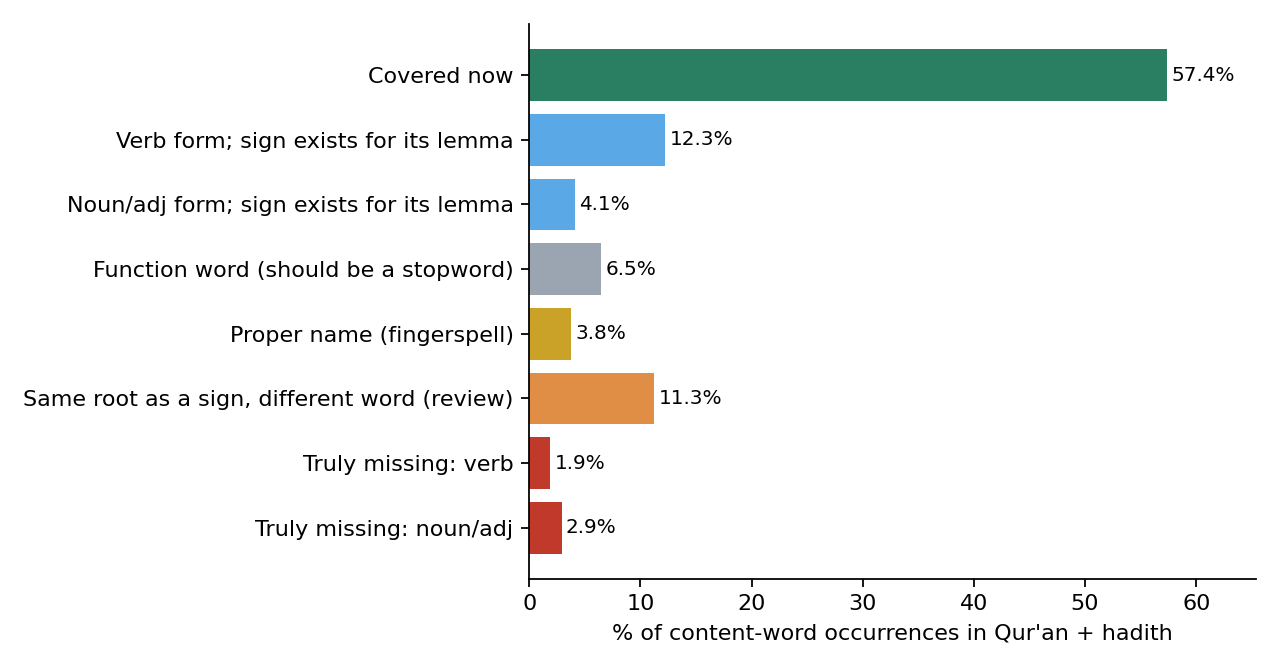
\includegraphics[width=0.85\textwidth]{figures/ar_missing_categories.png}
\caption{Arabic content-word occurrences by coverage status and reason for being uncovered.}
\label{fig:ar_missing}
\end{figure}

\paragraph{Matcher errors removed.} The audit also exposed false matches, which inflated the old figure:
\begin{itemize}[leftmargin=*,itemsep=2pt]
  \item \textbf{Article insertion.} To find forms such as \ar{وحج} $\to$ \ar{الحج}, the matcher tried ``\ar{ال} + stem''. That
    also turned \ar{وان} (\emph{and that}) into \ar{الوان}, which equals \ar{ألوان} (\emph{colours}) once hamza is folded: 1,692 false
    matches. An ``\ar{ال}'' form now counts only when the sign's gloss really begins with the article.
  \item \textbf{Section labels.} 3,574 hadith passages contain the label \ar{الشرح:} before their commentary, counted as a word;
    it is now removed before counting.
\end{itemize}
With these fixes the baseline is \textbf{57.1\,\%} (Qur'an 48.2\,\%, hadith 58.2\,\%), slightly below the earlier 57.4\,\%.

\paragraph{Synonyms.} Words without their own sign that ArSL signs with an existing sign of the same meaning are listed in a
reviewed table (\code{synonyms\_ar.json}, 86 entries), e.g.\ \ar{نكاح، تزويج} $\to$ \ar{زواج}, \ar{يصوم، صائم} $\to$ \ar{صوم},
\ar{بعير} $\to$ \ar{جمل}. Every entry is checked for its meaning in the Qur'an and hadith; a word that later gets its own sign keeps it.

\paragraph{Fingerspelling decided with a native signer.} After the expert rejected the recorded sign for \ar{عابد}
(Section~\ref{sec:annotators}), the word is fingerspelled letter by letter (\ar{ع ا ب د}) from the KArSL letter signs. 22 names of
the Companions (\ar{أبو بكر، عمر، عثمان، عائشة، فاطمة، أبو هريرة}, \ldots) are spelled the same way (pending review), and the same
names are spelled from one-signer alphabets in ASL and T\.{I}D. Names that collide with a common word are entered with their
honorific instead: \ar{علي} would collide with the preposition \ar{على}, so the entry is \ar{علي رضي الله عنه}, spelled and then followed by
the recorded honorific. Phrases a signer has recorded (\ar{عائشة رضي الله عنها}) are never replaced by a composed version.

\paragraph{Vetting the sources that were never merged.} Three sources had been collected but not merged, and were vetted before
merging. \textbf{SignBank} contributed no clips: all 861 rows reused clips already in the lexicon, many with the wrong sense (one clip
for \ar{الذكر}, \emph{remembrance}, and \ar{الرجل}, \emph{man}; \ar{الرسول} $\to$ \ar{سنة}), so only 67 genuine synonyms were kept and moved to
the synonym table. \textbf{ArabSign} sentences were checked for consistency across its six signers; 56 new glosses were accepted and
63 rejected because the gloss did not match the signed sentence. \textbf{Isharah} was withdrawn (Section~\ref{sec:lexicons}).

\paragraph{Inflection: verbs and nouns matched through their lemma.} The matcher deliberately matched verbs only in their
exact form, so that \ar{وتكفر} (\emph{expiates}) could not become \ar{كفر} (\emph{disbelief}); as a result \ar{قالت، قالوا، قلت}
missed the sign \ar{قال}, although ArSL signs the verb without its person or tense. Every corpus word and every gloss is now analysed
with CAMeL Tools (lemma, part of speech, clitics; cached), and a word reaches a sign through its lemma only under a meaning guard:
a verb form matches only a gloss whose own best reading is \emph{the same verb lemma}, and a noun form likewise; glosses not
spelled exactly as their lemma, words with a competing reading within 0.5 log-probability, and tanween forms (\ar{جدا} is not \ar{جد}) are
excluded. This guard removed false matches such as \ar{وسلم} $\to$ \ar{يسلم} and \ar{وجل} $\to$ \ar{فجل} (\emph{radish}), while
\ar{قالت، قالوا، قلت} $\to$ \ar{قال}, \ar{كانوا، يكون} $\to$ \ar{كان}, \ar{ربك، ربنا} $\to$ \ar{رب} and \ar{يده، بيده} $\to$ \ar{يد} now match, and
\ar{وتكفر}, \ar{إسلام} $\to$ \ar{سلام} and \ar{جنة} $\to$ \ar{جن} stay blocked. A quick check of 30 newly matched tokens, read in context,
found all 30 correct; a larger sample is planned, since out-of-context readings can still pick the wrong sense (\ar{يعرف} $\to$ \ar{عرّف}).

\paragraph{Stopwords and negation.} The stopword list grew from 60 to about 180 true function words (prepositions with attached
pronouns such as \ar{عنه، منه، إليه}, \ar{إلا، أنه، إنما، لعل}, conjunction combinations), so they no longer count as uncovered content.
Question words (\ar{لماذا، كيف، متى، أين، هل}) and negation (\ar{لا، لم، لن}) were removed from the list: they carry meaning and are now
signed. The audit found that negation had been silently dropped from signed sentences; \ar{لا} has no recorded sign yet and is
fingerspelled until one is recorded.

\paragraph{Result.} Over the new denominator (531,477 content tokens), Arabic coverage is \textbf{61.1\,\%} (Qur'an 54.4\,\%, hadith
61.9\,\%; distinct words 27.4\,\% $\to$ 32.1\,\%). Moving function words out of the denominator alone lowers coverage by 1.2 points, because
many of them were already matched; lemma matching adds 4.5 points (verbs 4.1, nouns 0.4). This is below the 73.7\,\% projected
from Table~\ref{tab:ar_missing} because the guards trade recall for precision.

\paragraph{Next: derivation and attached pronouns.} Two layers remain: a reviewed derivation table for the same root \emph{and}
the same meaning (\ar{الإجابة، فتجيبك} $\to$ \ar{جواب}; \ar{عابد، يعبد} $\to$ \ar{عبادة}), and attached pronouns signed after the word, as a
Deaf signer would (\ar{ربك} $\to$ \ar{رب} + \ar{أنت}; \ar{فتجيبك} $\to$ \ar{جواب} + \ar{هو}).

\section{Turkish and Urdu modes}
\begin{table}[ht]
\centering\small
\caption{Sign data for the Turkish and Urdu modes (status on 5 October 2026; the YouTube and PSL extractions are still running, so counts are lower bounds).}
\label{tab:trur}
\begin{tabularx}{\textwidth}{L{3.4cm} L{0.9cm} L{2.4cm} L{2.6cm} L{1.9cm} Y}
\toprule
Source & Lang. & Signs & Covers & Licence & Reference / Link \\
\midrule
T\.{I}D S\"ozl\"u\u{g}\"u~\cite{tidsozluk}\footnotemark & T\.{I}D & 1,374 (1,136 glosses) + 235 new & general dictionary, $\sim$5\,s clips & not stated & YouTube channel \\
TiDiSLaM Islamic terms\footnotemark & T\.{I}D & 175 & Islamic terms & not stated & YouTube channel \\
AUTSL~\cite{autsl} & T\.{I}D & 151 glosses (+ other signers as variants) & everyday words, 43 signers & research use & dataset \\
Opposite-pair re-cuts & T\.{I}D & 90 & see text & --- & derived from the dictionary \\
T\.{I}D alphabet + Companion names & T\.{I}D & 32 letters, 24 names & fingerspelling & not stated & one signer \\
\midrule
WSLP 2025~\cite{wslp,wslpislword}\footnotemark & ISL & 4,056 (4,020 glosses) & general words & CC BY-NC-ND & Hugging Face \\
CISLR v1.5-a~\cite{cislr}\footnotemark & ISL & 3,965 (46 religious) & dictionary, 1 clip/word & AFL-3.0 & Zenodo / GitHub \\
ISLRTC dictionary\footnotemark & ISL & 553 (484 new glosses) & government dictionary & not stated & YouTube channel \\
ISL alphabet & ISL & 26 letters (19 two-handed) & fingerspelling & not stated & one signer \\
FESF / Deaf Reach PSL dictionary\footnotemark & PSL & 242 so far (140 Islamic) of 6,516 & English + Urdu labels & \textcopyright\ FESF & behind a flag, not public \\
\bottomrule
\end{tabularx}
\end{table}
\addtocounter{footnote}{-6}%
\stepcounter{footnote}\footnotetext{T\.{I}D S\"ozl\"u\u{g}\"u YouTube channel: \url{https://www.youtube.com/channel/UCq2tlBndwWjJb2Zlf9QoOzQ}}%
\stepcounter{footnote}\footnotetext{TiDiSLaM Islamic terms in T\.{I}D: \url{https://www.youtube.com/channel/UC7zHDrJRMxSd65cE3vxfksg}}%
\stepcounter{footnote}\footnotetext{WSLP Indian Sign Language on Hugging Face: \url{https://huggingface.co/datasets/Exploration-Lab/WSLP}}%
\stepcounter{footnote}\footnotetext{CISLR dataset on GitHub: \url{https://github.com/cislr/cislr}}%
\stepcounter{footnote}\footnotetext{ISLRTC (Government of India) YouTube channel: \url{https://www.youtube.com/channel/UC3AcGIlqVI4nJWCwHgHFXtg}}%
\stepcounter{footnote}\footnotetext{Pakistan Sign Language dictionary (FESF / Deaf Reach): \url{https://psl.org.pk}}%

\paragraph{Turkish sources.} The first Turkish lexicon held 1,308 of the roughly 5,000 clips of the T\.{I}D dictionary
channel. We now download the whole channel and the TiDiSLaM Islamic-terms channel, words missing from the corpus first (Islamic
terms before others), then every other word, cutting each video to its first signing run with the same checks as the other
sources (0.4--4\,s, dominant hand visible in $\ge$70\,\% of frames, a single run). So far 347 clips were accepted and 116
rejected (mostly for a hand visible in too few frames). Islamic terms now signed include \textit{Allah, peygamber, namaz, abdest, ramazan,
iman, cennet, hadis, k\i{}yamet, secde}. AUTSL~\cite{autsl} adds 151 everyday glosses, with its other signers' recordings kept as
variants for recognition. The 189 Turkish videos listed in SignVerse-2M were screened from their metadata: 187 are continuous
signing (news, songs, lectures) and the two word lists repeat existing signs, so none was used.

\paragraph{Opposite pairs.} An audit found 66 dictionary clips shared by two opposite words (\textit{iyi}/\textit{k\"ot\"u},
\textit{var}/\textit{yok}, \ldots): each video signs both words, and the old cut kept only the first. Using the on-screen caption
change as the boundary, 90 of the 100 words were re-cut into their own clips (85 from the videos, 5 from AUTSL), checked on contact
sheets. Three words whose re-cut failed still showed their opposite (\textit{eksik}, \textit{ya\c{s}l\i}, \textit{\"ust}); they
were withdrawn, so they fall back to another source or to fingerspelling rather than signing the opposite.

\paragraph{Turkish morphology and synonyms.} Turkish is agglutinative, and the first matcher took a word's first five letters
as its stem. That missed short roots (\textit{geldi}~$\to$~\textit{gel}), consonant alternation (\textit{kitab\i}~$\to$~\textit{kitap})
and vowel drop (\textit{a\u{g}z\i}~$\to$~\textit{a\u{g}\i z}), and it made confident errors: \textit{sallallahu} matched
\textit{sallanmak} (to swing), about 8,300 wrong matches on its own. The matcher now lemmatises both corpus tokens and glosses
with Zemberek (the \texttt{zeyrek} port), prefers the reading whose lemma is a gloss, and keeps a prefix fallback only for words
the analyser does not know. A reviewed synonym table (36 entries, e.g.\ \textit{rasul/resul}~$\to$~\textit{peygamber},
\textit{tevbe}~$\to$~\textit{t\"ovbe}, \textit{mescit/cami}~$\to$~\textit{mescid}) follows the same rules as the Arabic one; uncertain
pairs are left out (\textit{tanr\i}, \textit{ilah}; \textit{salat}~$\to$~\textit{namaz} is excluded because \textit{salat} in this
corpus is the blessing on the Prophet). On the same lexicon, content-token coverage rose from 38.3\,\% to 53.9\,\% (Qur'an 37.6\,\%
$\to$ 58.3\,\%, hadith 38.4\,\% $\to$ 53.0\,\%). A quick precision check found the synonym route correct on 8 of 8 samples and the
lemma route on 12 of 14 (errors: \textit{alt\i nla}, ``with gold'', $\to$ \textit{alt}; \textit{olmazlarsa}~$\to$~\textit{olmaz}).

\paragraph{Urdu mode: ISL and PSL.} Indian Sign Language stands in for the Urdu mode because it has the largest open data among the
nearest sign languages. ISLRTC adds 553 signs (484 new glosses), raising ISL content-token coverage from 51.1\,\% to 55.5\,\%, and
a one-signer ISL alphabet makes fingerspelling of names possible (most letters are two-handed, so both hands are kept). Since most Urdu
speakers use Pakistan Sign Language, we added the FESF / Deaf Reach PSL dictionary, which labels 6,516 concepts in English and
Urdu. With the 242 PSL signs extracted so far (140 Islamic, e.g.\ \textit{hajj, wudu, roza, zakat, masjid}), coverage of the Urdu-mode
passages rises from 55.5\,\% to 70.4\,\%. The site is ``all rights reserved'', so PSL stays behind a flag and is not public until
FESF agrees. The 3,023 Indian and 581 Pakistani SignVerse-2M videos screened so far are news bulletins and stories, unusable for word signs.
Whether ISL or PSL signs suit Pakistani Deaf viewers must be checked with them. iSign~\cite{isign} (ISL sentence translation, CC
BY-NC-SA 4.0) is noted for future recognisers.

\section{Exploratory analysis}
Figure~\ref{fig:lexsrc} shows how each lexicon is composed. The ASL lexicon is dominated by ASL Citizen, a single
consistent dictionary; the ArSL lexicon draws on ten sources of different dialects and recording styles, which is why
body proportions must be normalised (Section~\ref{sec:render}). Figure~\ref{fig:lengths} shows sign durations: the median
ASL sign lasts 1.64\,s (41 frames) and the median ArSL sign 2.08\,s (52 frames). Sources cut from continuous signing
(Qur'an curriculum, Tawasol, Levantine Shorts, explained dictionaries: medians 0.7--1.4\,s) are shorter than dictionary
clips, which include the hand rising and falling (scouts' dictionary: 3.9\,s). All recordings are trimmed to the
hand-visible span; in raw KArSL clips the dominant hand is missing in half of the frames (median missing ratio 0.50),
which shows why trimming matters.

\begin{figure}[ht]
\centering
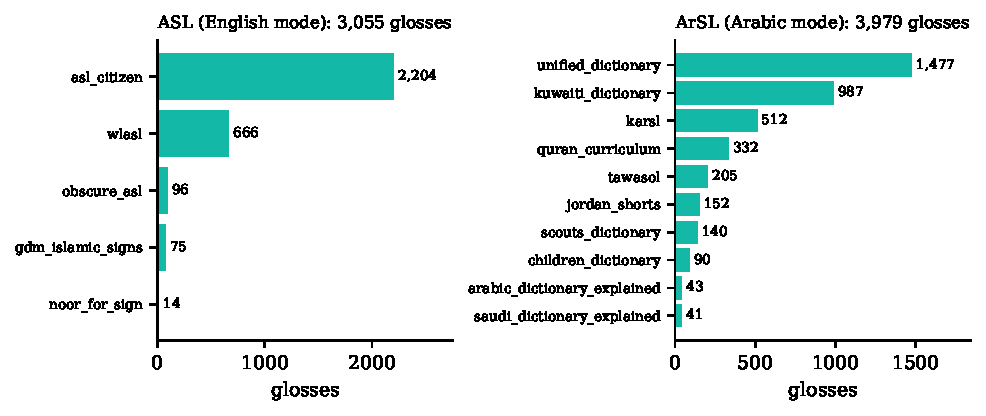
\includegraphics[width=\textwidth]{figures/lexicon_sources.pdf}
\caption{Distinct glosses contributed by each source to the merged lexicons (after removing duplicates; first source
wins).}
\label{fig:lexsrc}
\end{figure}

\begin{figure}[ht]
\centering
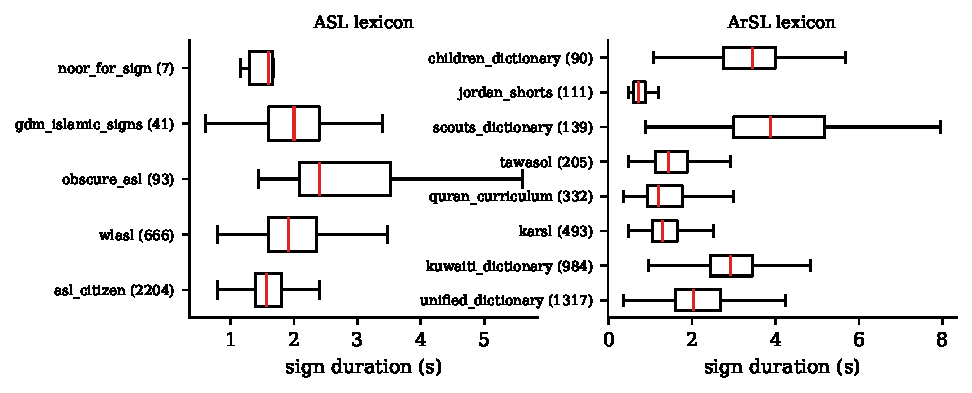
\includegraphics[width=\textwidth]{figures/sign_lengths.pdf}
\caption{Sign duration per source (box: quartiles, line: median; number of recordings in brackets). 25 fps.}
\label{fig:lengths}
\end{figure}

\begin{table}[ht]
\centering\small
\caption{Pose statistics of the merged lexicons (frames at 25 fps; one row per distinct recording).}
\label{tab:posestats}
\begin{tabular}{l r r r r r r r}
\toprule
Lexicon & Recordings & Mean & Median & P5 & P95 & Min & Max \\
\midrule
ASL (English mode) & 3,288 & 44.8 & 41 & 28.5 & 76 & 15 & 228 \\
ArSL (Arabic mode) & 3,755 & 55.6 & 52 & 18 & 104.3 & 9 & 223 \\
Isharah Mined Signs (ArSL) & 1,113 & 134.2 & 128 & 36 & 210 & 16 & 280 \\
T\.{I}D (so far) & 1,308 & 68.2 & 67.5 & 44 & 94 & 23 & 128 \\
ISL, WSLP & 4,056 & 256.2 & 219 & 43 & 627 & -- & 744 \\
ISL, CISLR & 3,965 & 85.8 & 57 & 31 & 270 & -- & 359 \\
ArabSign sentences & 9,259 & 98.2 & 95 & 52 & 159 & 33 & 259 \\
\bottomrule
\end{tabular}
\end{table}

\section{Continuous Lexicon Mining from the Full Isharah Corpus (v1 and v2)}
\label{sec:isharah_full_mining}

To maximize vocabulary coverage for continuous Saudi and Gulf Arabic signing beyond isolated dictionary poses, we executed our pre-trained RoPE Transformer segmentation pipeline across the \textbf{entire Isharah continuous corpus}, processing both Version~1 (10,450 sentences) and Version~2 Phase~1 (21,450 sentences) across training, validation, and testing splits.

Unlike prior experiments limited to a 3,000-sentence subset, scaling to all 21,450 continuous sentences yielded:
\begin{enumerate}[leftmargin=*,itemsep=2pt]
  \item \textbf{Total Physical Signs Segmented:} 34,455 discrete kinematic gesture segments extracted at frame level.
  \item \textbf{Exact 1-to-1 Sentence Matches:} 1,055 sentences where detected physical gesture boundaries matched transcript gloss lengths with zero misalignment.
  \item \textbf{Comprehensive Vocabulary Coverage:} \textbf{1,113 unique vocabulary glosses} mined from continuous sentences, spanning everyday communication, question particles (\ar{سوال، استفهام}), pronouns (\ar{انا، هو}), and core verbs (\ar{رغبه، ذهاب، اكل، شراء}).
  \item \textbf{Consensus-Verified Canonical Prototypes:} 1,079 glosses met the strict multi-signer consensus threshold ($\ge 5$ independent occurrences across $\ge 3$ unique Deaf signers), yielding high-confidence canonical sign medoids with natural motion envelopes.
\end{enumerate}
This full-corpus extraction adds 1,113 authenticated, continuous-derived gestures into the Isharati ArSL repository, drastically mitigating the out-of-vocabulary rate for colloquial and religious sentence translation.

\chapter{Exploratory analysis of the corpora and lexicons}
\label{sec:eda}

This section describes the data the system signs from, before any result is reported: how large each corpus is,
which words dominate it, how much of it each lexicon can sign, and which sources supply the signs.

\section{The corpora}
Table~\ref{tab:eda_corpora} compares the four corpora. All share the same 6,236 verses; the hadith sets differ because
not every hadith of the encyclopedia is translated into every language. The hadith make up most of the text (80--89\% of
tokens), since each carries a title and a scholarly explanation. The Arabic corpus has more than four times the distinct
words of the English one (62,613 against 13,612) for fewer tokens, because Arabic writes conjunctions, prepositions and
pronouns as part of the word; Turkish, an agglutinative language, shows the same effect (49,131 distinct words). Lexicon
matching therefore has to reduce words to their stems (Section~\ref{sec:glossing}), and distinct-word coverage is a poor
guide for these two languages; occurrence coverage is the figure we report.

\begin{table}[ht]
\centering\small
\caption{The four knowledge corpora: size, and the share of content-word occurrences that the sign lexicon of
each mode can sign. Urdu answers are signed with Indian Sign Language, whose glosses are English words, so its
coverage is measured on the English corpus of the same verses and hadith.}
\label{tab:eda_corpora}
\begin{tabular}{l r r r r r r}
\toprule
Mode & Passages & Tokens & Distinct words & Content tokens & Qur'an covered & Hadith covered \\
\midrule
English / ASL & 8,564 & 865,157 & 13,612 & 425,556 & 84.4\% & 80.3\% \\
Arabic / ArSL & 9,810 & 727,335 & 62,613 & 595,022 & 46.3\% & 54.1\% \\
Turkish / T\.{I}D & 8,386 & 606,797 & 49,131 & 498,831 & 15.8\% & 16.0\% \\
Urdu / ISL & 8,456 & 942,554 & 18,035 & 569,880 & 54.4\% & 50.4\% \\
\bottomrule
\end{tabular}
\end{table}

\begin{table}[ht]
\centering\small
\caption{The ten most frequent content words of the Qur'an and of the hadith in each corpus (tokens of two
letters or fewer, mostly clitic fragments, are not shown). $^\dagger$: no sign in that mode's lexicon.}
\label{tab:eda_top}
\begin{tabularx}{\textwidth}{l l Y}
\toprule
Corpus & Part & Most frequent content words \\
\midrule
English & Qur'an & allah (2,976), not (2,194), indeed (1,498), lord (972), said (821), say (767), people (740), upon (627), day (500), among (474) \\
 & Hadith & allah (20,607), upon (8,496), peace (7,724), blessings (7,539), said (6,828), prophet (5,704), not (5,130), one (3,808), messenger (3,694), pleased (3,499) \\
\addlinespace
Arabic & Qur'an & \ar{الله} (2,155), \ar{الا}$^\dagger$ (763), \ar{ولا}$^\dagger$ (658), \ar{قال} (416), \ar{لهم} (373), \ar{لكم} (337), \ar{وان} (323), \ar{بما} (296), \ar{الارض} (287), \ar{امنوا} (263) \\
 & Hadith & \ar{الله} (31,590), \ar{عليه} (15,902), \ar{صلي} (12,894), \ar{وسلم}$^\dagger$ (12,493), \ar{قال} (9,013), \ar{النبي} (6,583), \ar{رسول} (5,569), \ar{رضي} (4,952), \ar{فقال}$^\dagger$ (3,831), \ar{عنه}$^\dagger$ (3,709) \\
\addlinespace
Turkish & Qur'an & allah$^\dagger$ (3,092), iman (602), size (589), onların (569), onlara$^\dagger$ (566), şüphesiz (565), işte (500), eğer$^\dagger$ (470), onu$^\dagger$ (451), onları (446) \\
 & Hadith & aleyhi$^\dagger$ (8,394), sallallahu (8,345), sellem$^\dagger$ (8,319), allah$^\dagger$ (7,514), radıyallahu$^\dagger$ (4,171), şöyle$^\dagger$ (4,050), rasûlullah$^\dagger$ (3,673), anh$^\dagger$ (2,820), dedi$^\dagger$ (2,454), nebi$^\dagger$ (2,269) \\
\addlinespace
Urdu & Qur'an & \ar{اللہ} (3,121), \ar{تعالی} (1,552), \ar{اپنے} (1,108), \ar{واﻻ} (852), \ar{پھر} (829), \ar{لوگ} (795), \ar{کوئی} (727), \ar{انہیں} (706), \ar{کرتے} (675), \ar{طرف} (642) \\
 & Hadith & \ar{اللہ} (19,536), \ar{رضی} (5,502), \ar{فرمایا} (4,110), \ar{رسول} (3,991), \ar{عنہ} (3,724), \ar{نبی} (3,660), \ar{اسے} (3,332), \ar{اپنے} (3,273), \ar{پھر} (3,024), \ar{کوئی} (2,602) \\
\addlinespace
\bottomrule
\end{tabularx}
\end{table}

\begin{table}[ht]
\centering\small
\caption{The signs used most often when the Qur'an and hadith are signed: the share of all content-word
occurrences that each sign covers.}
\label{tab:eda_signs}
\begin{tabularx}{\textwidth}{l Y}
\toprule
Lexicon & Most used signs (share of content-word occurrences) \\
\midrule
ASL & ALLAH (5.7\%), SAY (2.5\%), UPON (2.1\%), PEACE (1.8\%), BLESSINGS (1.8\%), NOT (1.7\%), PROPHET (1.4\%), ONE (1.0\%), MESSENGER (1.0\%), PLEASE (0.8\%), PEOPLE (0.7\%), REPORT (0.6\%), EXPLANATION (0.6\%), O (0.5\%), MAN (0.5\%) \\
ArSL & \ar{الله} (5.9\%), \ar{على} (3.2\%), \ar{صلى} (2.2\%), \ar{قال} (1.7\%), \ar{أن} (1.5\%), \ar{نبي} (1.2\%), \ar{رسول} (1.1\%), \ar{رضي} (0.9\%), \ar{له} (0.8\%), \ar{شرح} (0.6\%), \ar{فئة} (0.5\%), \ar{أب} (0.5\%), \ar{رجل} (0.5\%), \ar{الصلاة} (0.4\%), \ar{يوم} (0.4\%) \\
\bottomrule
\end{tabularx}
\end{table}


\section{Frequent words}
Table~\ref{tab:eda_top} lists the most frequent content words. Three patterns hold across languages. First, the name of
God (\emph{Allah}, \ar{الله}, \emph{Allah}, \ar{اللہ}) is the most frequent word of every corpus, so a single sign
already covers a large share of the text. Second, the hadith are dominated by the formulas of transmission and respect:
``peace and blessings be upon him'' (\ar{صلى الله عليه وسلم}, \emph{sallallahu aleyhi ve sellem}, \ar{ﷺ}), ``may Allah be
pleased with him'' (\ar{رضي الله عنه}, \emph{rad\i{}yallahu anh}), and verbs of narration (\emph{said, reported};
\ar{قال}; \emph{dedi, rivayet}). In sign language these formulas are signed as fixed units, not word by word, so they are
the cheapest gaps to close. Third, the Qur'an's frequent words are its theological vocabulary (\emph{Lord, day, people,
believe}; \ar{الأرض، آمنوا}), which overlaps with general dictionaries more than the vocabulary of the hadith
explanations does.

\section{How much each lexicon can sign}
Figure~\ref{fig:covlang} shows the share of content-word occurrences that each mode can sign today. English/ASL is the
most complete (64\% of the Qur'an, 63\% of the hadith), followed by Arabic/ArSL (46\% and 54\%). The Arabic Qur'an is
harder than the Arabic hadith because classical Qur'anic forms are rarer in dictionaries; the Qur'an-curriculum signs
partly offset this.

\paragraph{Turkish.} The T\.{I}D lexicon is still being extracted: 1,308 of the 5,017 dictionary clips have been
converted (980 single-word glosses), and the Islamic-terms channel has not been processed yet. It covers 16\% of
content-word occurrences, and its most frequent gaps are exactly the religious words: \emph{Allah, aleyhi, sellem,
rad\i{}yallahu, ras\^{u}lullah, nebi} (prophet), \emph{rivayet} (narration). A general dictionary does not contain the
vocabulary of religious texts, which is why the Islamic-terms source matters more than its 589 clips suggest.

\paragraph{Urdu.} The Indian Sign Language lexicons (5,181 single-word glosses) cover 51\% of content-word occurrences
of the same texts, measured on the English glosses. Their gaps show the same pattern: \emph{peace, blessings, prophet,
prayer, Lord} have no ISL sign in these general-purpose datasets, so the Urdu mode cannot sign a basic answer until
Islamic terms are added.

\begin{figure}[ht]
\centering
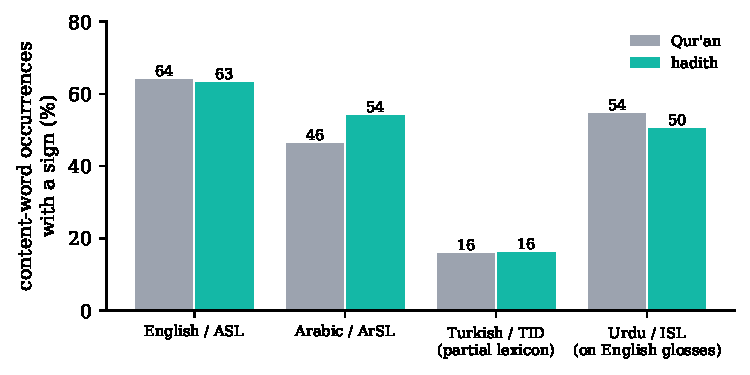
\includegraphics[width=0.72\textwidth]{figures/coverage_languages.pdf}
\caption{Content-word occurrences of the Qur'an and hadith that each mode's lexicon can sign.}
\label{fig:covlang}
\end{figure}

\section{Which sources supply the signs}
Figure~\ref{fig:attribution} attributes every covered occurrence to the source of the sign the matcher returns. In
English, ASL Citizen supplies 40.5\% of the content-word occurrences through 1,234 different signs, while the 40 GDM
Islamic signs supply 10.2\%: forty religious signs do a quarter of the work of a 2,204-sign general dictionary. In Arabic
the effect is stronger: the 324 signs cut from the Qur'an curriculum cover 28.8\% of all content-word occurrences, more
than KArSL, the unified dictionary and the Kuwaiti dictionary together (22.3\%). Dictionaries of everyday vocabulary
(children's, scouts', Levantine) contribute below 1\% each. Table~\ref{tab:eda_signs} lists the individual signs used
most: \ar{الله} alone signs 5.9\% of all Arabic content-word occurrences (ALLAH: 5.7\% in English), followed by
\ar{على}, \ar{صلى} and \ar{قال}, which come from the hadith formulas. Two
conclusions follow for collecting data: a small set of religious signs recorded by Deaf signers is worth more than a large
general dictionary, and the hadith formulas should be recorded as phrase signs.

\begin{figure}[ht]
\centering
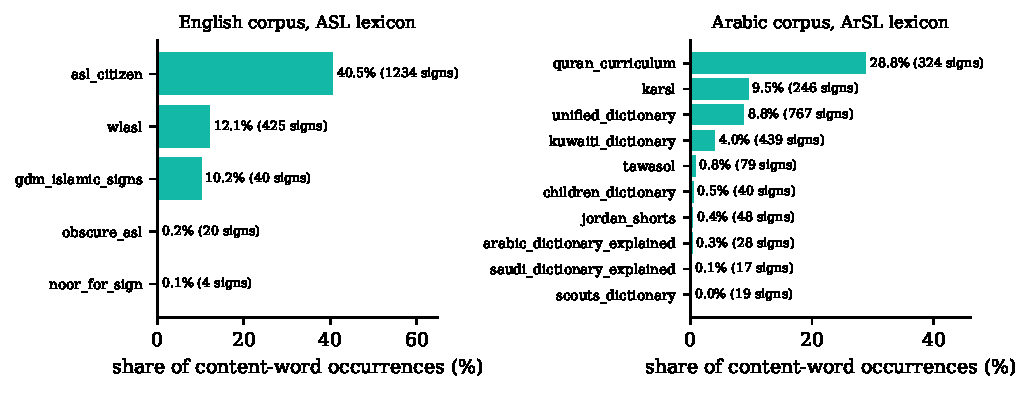
\includegraphics[width=\textwidth]{figures/source_attribution.pdf}
\caption{Share of the corpus's content-word occurrences signed by each lexicon source (in brackets, the number of that
source's signs that are used).}
\label{fig:attribution}
\end{figure}

\chapter{Signed scripture corpora: the Qur'an and the hadith}
\label{sec:scripture}

The lexicons of Chapter~\ref{sec:lexicons} hold single signs. This chapter describes the continuous signing of whole
ayat and hadith by human signers: five Qur'an datasets and a new signed hadith corpus, how each sample was labelled,
what the data contain, and the quality problems we found in all of them and corrected. Every figure comes from the
published builds and the pipeline state of 6 October 2026, computed by \code{docs/paper/tools/scripture\_eda.py}. The
hadith corpus was still growing on that date; the figures are a snapshot.

\section{Five signed Qur'an datasets}
\label{sec:quran_sets}

Table~\ref{tab:quran_sets} lists the five Qur'an datasets now published, two more than Section~\ref{sec:lexicons}
described. For the three YouTube sources (King Fahd Complex, al-Mukhtasar fi Tafsir, Al-Kharj curriculum), Whisper
\cite{whisper} supplies only the timing; each segment's label is the fixed Uthmani text, aligned to the timed
transcript, so a recognition error never becomes a label. Tebyan\footnote{Tebyan Qur'an: \url{https://tebyanquran.com}}
publishes one clip per ayah (some clips cover several), so its labels are the publisher's own. Diyanet's two Qur'an
episodes in Turkish Sign Language\footnote{Diyanet \.{I}\c{s}leri Ba\c{s}kanl\i\u{g}\i, ``\.{I}\c{s}aret Dili ile
Kur'an'', YouTube playlist PLtApkPE49w-tQ8-zFm1QVrwrmYKauonS9.} gave a false alignment, because Whisper caught the
spoken basmala of the introduction; their labels come from the text panels the publisher shows while each phrase is
signed.

\begin{table}[ht]
\centering
\small
\caption{The five signed Qur'an datasets as published (private Hugging Face datasets). A segment is one ayah's recitation or one passage of tafsir; hours are the signed time.}
\label{tab:quran_sets}
\begin{tabular}{llrrrrrr}
\toprule
Source & SL & Segments & Recitation & Tafsir & Ayahs & Surahs & Hours \\
\midrule
King Fahd Complex & ArSL & 1,066 & 592 & 468 & 558 & 38 & 7.4 \\
al-Mukhtasar fi Tafsir & ArSL & 6,127 & 0 & 6,092 & 5,916 & 112 & 34.7 \\
Al-Kharj curriculum & ArSL & 207 & 207 & 0 & 186 & 22 & 0.3 \\
Tebyan & ArSL & 567 & 567 & 0 & 570 & 38 & 2.4 \\
Diyanet & TİD & 13 & 13 & 0 & 12 & 2 & 0.1 \\
\bottomrule
\end{tabular}
\end{table}


Together the five datasets hold 7,980 labelled segments and about 44.9 hours of signing. Al-Mukhtasar alone covers 5,916
ayat of 112 surahs, almost all as tafsir: the signer explains each ayah rather than reciting it. Each dataset is a
private Hugging Face repository with a manifest (one row per segment, with its YouTube timestamp), the full MediaPipe
Holistic keypoints and the same motion as Isharati poses; no video is redistributed. In the application each ayah can
be played by any of the signers that cover it (Section~\ref{sec:scripture_app}).

\section{A signed hadith corpus}
\label{sec:hadith_corpus}

Section~\ref{sec:intro} motivated Isharati partly by the absence of a hadith collection in sign language. That claim
needs a correction: signed hadith exist, in some quantity, on YouTube, made by Deaf associations and educational
channels. What does not exist is a collection that can be searched, aligned to the hadith text or used to train and
drive a signing model. We built one.

\subsection{Sources}
A search of YouTube for hadith in sign language (Arabic and Turkish queries) found 14 sources: playlists and channels
of Islamweb for Deaf\footnote{\url{https://www.youtube.com/channel/UCf61i7CZLHYBSm3wz7dY_yg}}, the Insan association's
Nawawi's Forty in sign language, the Deaf Educational Channel\footnote{\url{https://www.youtube.com/channel/UC86B8NmyJ4n4PkUhLpkAP9Q}}
(Umdat al-Ahkam, Riyad al-Salihin, thirty hadith for women and a Nawawi series), three Deaf preachers' Nawawi lessons,
and two Turkish sources (``\.{I}\c{s}aret Dili ile 40 Hadis''). In all, 824 videos and 114.4 hours. They come in two
kinds: \emph{clips}, one hadith per video, often under five minutes, and \emph{lessons}, a signed explanation of one
hadith that can last an hour. Videos are streamed: each is downloaded, transcribed, matched and reduced to keypoints, and
then deleted, so the corpus keeps only keypoints and links.

\subsection{Labelling: the label is always the collection's text}
\label{sec:hadith_labels}
A label is a hadith as printed in its collection, taken from the open hadith-api \cite{hadithapi} (Bukhari, Muslim, Abu
Dawud, Tirmidhi, Nasa'i, Ibn Majah, Malik, Nawawi's Forty and the Qudsi hadith, in Arabic, English and Turkish). A
transcript or an on-screen text only says \emph{which} hadith a video signs; it never becomes the label. Four routes lead
to a label, chosen by what the video offers:

\begin{enumerate}[leftmargin=*,itemsep=2pt]
  \item \textbf{Voice-over.} Where an interpreter reads the hadith aloud, a local Whisper large-v3-turbo model gives word
        timestamps, and the transcript is matched word by word against the collections (a word-bigram index weighted by
        inverse document frequency proposes candidates; an ordered alignment confirms them). A match needs at least
        8 words in order, at least 55\% of the transcript words inside the span, and at least 3 distinctive word pairs.
        The last condition was added after a chain of narrators alone (``\ar{عن أبي هريرة رضي الله عنه قال قال رسول الله}'')
        matched dozens of unrelated hadith. The span where the text is read is kept as \code{read\_start}, \code{read\_end}.
  \item \textbf{Translation.} The Turkish voice-overs paraphrase a translation, so word matching fails. A language model
        names the Arabic hadith and the time span, and the Arabic collections must confirm the proposed text, or the
        proposal is dropped.
  \item \textbf{On-screen text.} 450 of the 638 videos transcribed so far (71\%) are silent or carry only room noise:
        Deaf-made content often has no voice. Most show the hadith on screen, so a vision model reads the text from a
        few frames and the collections confirm it. The model matters: a smaller model, given a decorative font, returned
        the text of a famous hadith instead of the one on screen, which the collections then confirmed. A larger model
        read it correctly, and every such label is cross-checked against the hadith number in the title; a disagreement
        is flagged, not resolved silently.
  \item \textbf{Title.} A silent clip whose screen cannot be read keeps the publisher's number from its title (for
        Nawawi's Forty, the text follows from the number). An early parser read ``\ar{الحديث الثاني | الأربعون النووية}''
        as hadith 42; the fixed parser stops at the separator, and 31 title references were corrected.
\end{enumerate}

\subsection{Keypoints and the signer's face}
Each sample is a whole clip, trimmed to the frames in which the signer is visible, or, in a voiced lesson, the span
where a hadith is read. MediaPipe Holistic \cite{mediapipeholistic} gives pose, hands and the 478-point face mesh for
every frame; the same pass now also keeps the 52 face blendshape scores (brows, eyes, mouth), so the avatar can carry
the signer's facial expression and the skeleton view can draw the face. The face is published as 160 contour points on
the same 25\,fps frames as the Isharati pose, centred on the neck and in shoulder widths like the body.

\subsection{What the corpus contains}
\begin{table}[ht]
\centering
\small
\caption{Signed hadith samples per source in the published snapshot (6 October 2026). Labelled samples carry a hadith verified against its collection; hours are the signed time after trimming.}
\label{tab:hadith_sources}
\begin{tabular}{llrrrr}
\toprule
Source & SL & Samples & Labelled & Distinct hadith & Hours \\
\midrule
Deaf Educational Ch., Umdat al-Ahkam & ArSL & 134 & 129 & 128 & 6.55 \\
Islamweb for Deaf & ArSL & 103 & 95 & 59 & 3.91 \\
Insan, Nawawi's Forty & ArSL & 52 & 50 & 50 & 1.03 \\
Deaf Educational Ch., Riyad & ArSL & 26 & 19 & 19 & 1.20 \\
H. Wadwid, hadith & ArSL & 24 & 8 & 8 & 0.98 \\
E. Demir, 40 Hadis (TİD) & TİD & 23 & 18 & 17 & 0.07 \\
Deaf Educational Ch., 30 for women & ArSL & 19 & 15 & 15 & 1.18 \\
M. Hafez, Nawawi's Forty & ArSL & 15 & 15 & 15 & 0.26 \\
TİD, single videos & TİD & 5 & 0 & 0 & 0.14 \\
ArSL, single videos & ArSL & 3 & 2 & 2 & 0.04 \\
\midrule
Total & & 404 & 351 & 282 & 15.37 \\
\bottomrule
\end{tabular}
\end{table}


\begin{figure}[ht]
\centering
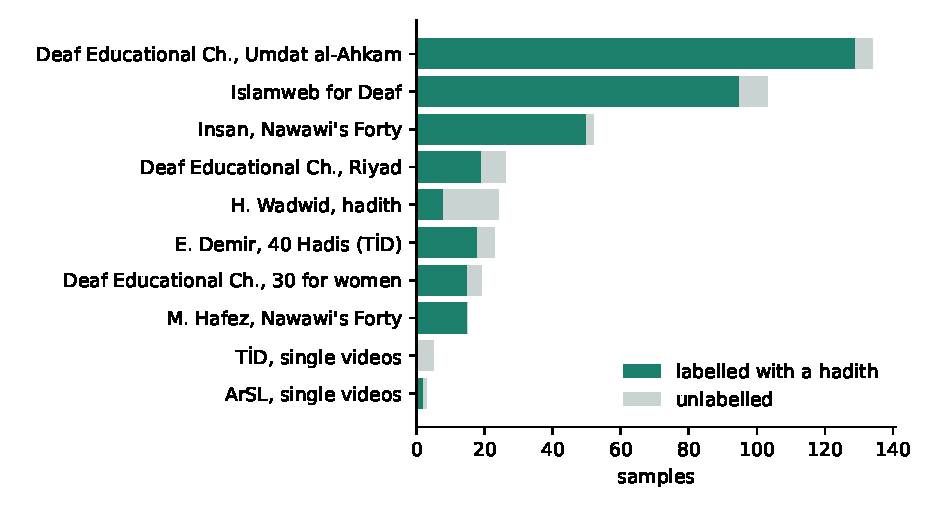
\includegraphics[width=0.92\textwidth]{figures/hadith_sources.pdf}
\caption{Signed hadith samples per source in the published snapshot. The grey part of each bar has no verified label
(it is hidden in the application).}
\label{fig:hadith_sources}
\end{figure}

The snapshot holds 404 samples and 15.4 hours of signing. 351 samples (87\%) carry a verified hadith, 333 in ArSL and
18 in T\.{I}D, covering 282 distinct hadith. The routes of Section~\ref{sec:hadith_labels} contributed 185 labels from
on-screen text, 146 from voice-overs, 18 from translations and 2 from titles alone; for 218 labels the publisher's
title agrees with the text match. Figure~\ref{fig:hadith_collections} shows where the labels come from: Bukhari (133)
and Muslim (69) dominate, as the sources teach the canonical hadith, and Nawawi's Forty is complete but for one
hadith (41 of 42). Most hadith have one signer (229); 53 have two to five, which is what a comparison between signers
needs. The signer is detected in 88\% of frames, the hands in 62\% (a hand at rest is often outside the frame), the face
in 79\%; 364 samples carry the blendshape scores.

\begin{figure}[ht]
\centering
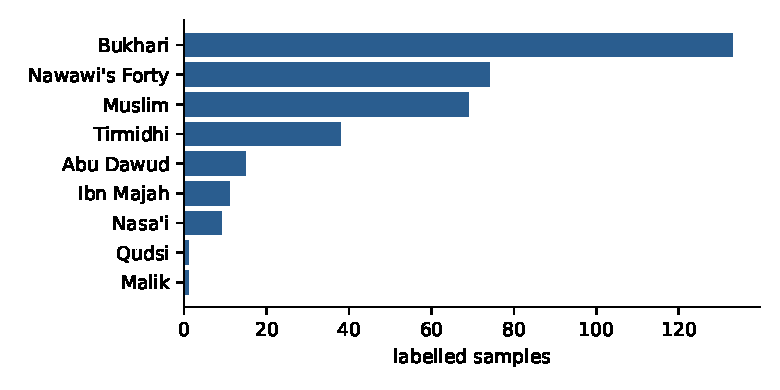
\includegraphics[width=0.72\textwidth]{figures/hadith_collections.pdf}
\caption{Collection of each verified hadith label. A hadith in several collections is counted once, under the collection
whose text matched best (Nawawi's Forty first for the Nawawi series).}
\label{fig:hadith_collections}
\end{figure}

Four lesson series (65.7 hours) are listed but not yet in the snapshot. The two transcribed so far are silent, so they
need the on-screen route, and a lesson yields one sample per hadith rather than per video.

\subsection{Gloss targets}
Each hadith also gets a sentence-level gloss, made by the application's own lexicon-constrained glossers (ArSL for the
Arabic text, T\.{I}D for the Turkish translation). The glosser is given the Prophet's words only: the chain of narrators
and the source note (``\ar{رواه البخاري}'') are cut first, a step that needed two fixes (an HTML line break before the
source note, and hadith in which a companion asks a question and no ``\ar{قال رسول الله}'' marks the start). Of the 206
ArSL glosses, the median share of words with no recorded sign is 33\%; of the 12 T\.{I}D glosses, 7\%. These glosses
are a text-to-sign target, not an annotation of what the human signer did: the signer's own choice and order of signs
differ, and a gloss is shown in the application only under a signer of the same sign language.

\section{Pose quality across all signed datasets}
\label{sec:pose_qa}

A visual check of the hadith samples in the application found skeletons that looked stretched, and an avatar whose arm
folded into its face. An automatic check of every published sample (\code{scripts/eval/qa\_sign\_datasets.py}: body
proportions, joint jumps, hand-to-wrist distance, face alignment, labels and glosses) showed that the problem was not
limited to the hadith.

\paragraph{Square units.} MediaPipe returns $x$ as a share of the frame's width and $y$ as a share of its height. On a
16:9 video one unit of $x$ is 1.78 units of $y$, so a pose normalised by shoulder width came out stretched tall: the
upper arm measured 1.25--1.44 shoulder widths, where an adult's is about 0.7--0.9. Every published pose is now built
from $x \cdot w/h$, with $w/h$ taken from each video (the clip's metadata, or the downloader's record of the
downloaded format), and a pose whose frame size is unknown is refused rather than published stretched.

\paragraph{Glitches and wrong figures.} A joint that sits more than 0.5 shoulder widths from the median of its seven
neighbouring frames is blanked and interpolated (real signing does not move a wrist that far and back within a few
frames). Frames whose shoulder width is far from the clip's own (0.6--1.6 times the median) are dropped at the ends of
a clip and interpolated inside it: they were introduction and closing cards in which a small figure, or a book cover,
was detected instead of the signer.

\begin{table}[ht]
\centering
\small
\caption{Pose quality before and after the two corrections, on a random sample of clips per dataset. Upper arm over shoulder width is about 0.7--0.9 in adults; a jump is a body joint moving more than 0.6 shoulder widths between two frames at 25\,fps.}
\label{tab:pose_qa}
\begin{tabular}{lrrrrr}
\toprule
& & \multicolumn{2}{c}{Upper arm / shoulder} & \multicolumn{2}{c}{Jumps per 100 frames} \\
\cmidrule(lr){3-4}\cmidrule(lr){5-6}
Dataset & Clips & raw units & square units & before filter & after filter \\
\midrule
King Fahd Complex & 60 & 1.41 & 0.87 & 0.19 & 0.10 \\
al-Mukhtasar fi Tafsir & 60 & 1.42 & 0.86 & 0.13 & 0.04 \\
Al-Kharj curriculum & 60 & 1.29 & 0.81 & 0.05 & 0.05 \\
Tebyan & 60 & 1.39 & 0.84 & 0.41 & 0.21 \\
Diyanet & 13 & 1.25 & 0.77 & 0.01 & 0.00 \\
Signed hadith & 120 & 1.32 & 0.83 & 2.96 & 1.75 \\
\bottomrule
\end{tabular}
\end{table}


\begin{figure}[ht]
\centering
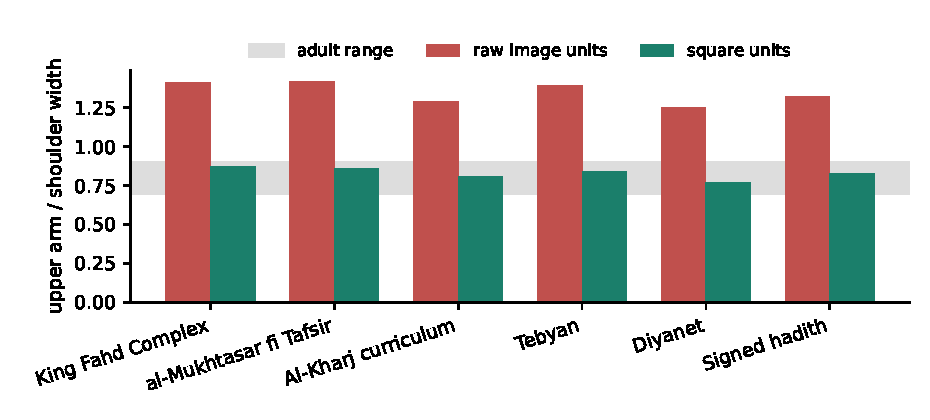
\includegraphics[width=0.92\textwidth]{figures/pose_aspect_qa.pdf}
\caption{Upper arm over shoulder width, median over a random sample of clips per dataset, in raw image units and in
square units. The grey band is the adult range.}
\label{fig:pose_aspect_qa}
\end{figure}

Table~\ref{tab:pose_qa} and Figure~\ref{fig:pose_aspect_qa} show the effect on a random sample of each dataset: every
dataset moves into the adult range (0.77--0.87), and the spike filter halves the joint jumps where they were frequent
(hadith 2.96 to 1.75 per 100 frames, Tebyan 0.41 to 0.21). Over every published sample, the upper arm was out of
the adult range in 1,036 of 1,066 King Fahd segments, 550 of 567 Tebyan, 203 of 207 Al-Kharj and all 13 Diyanet
segments before the correction, and in 4 King Fahd segments after it. What the check still flags is mostly motion,
not shape: joint jumps in 133 of the 404 hadith samples (most in the seated Umdat al-Ahkam lessons, where the
sheikh turns and leans) and in under 1\% of the Qur'an segments; a hand drifting from its wrist in 16 hadith samples,
126 King Fahd, 56 Tebyan and 171 of the 6,127 al-Mukhtasar segments.

\paragraph{The lexicon had the same bias.} The lexicon does not keep each video's aspect, but it already rescaled every
sign to one body shape (Section~\ref{sec:lexicons}): the nose-to-neck height over shoulder width was set to 0.74, the
median of ASL Citizen. That median was measured on 4:3 webcam frames, so every lexicon sign was normalised to a body
about 1.5 times too tall. In square units the five datasets above give 0.47--0.55; the lexicon reference is now 0.50.

\section{Retargeting to realistic avatars}
\label{sec:retarget_realistic}
The realistic avatars (Rocketbox, Section~\ref{sec:avatars}) did not bend their elbows in signs that need it. On
\ar{وضوء} (KArSL sign 0381), the signer's right elbow is at 104\textdegree{} (180\textdegree{} is straight), the cartoon
avatar's at 90\textdegree{}, and the Rocketbox avatars' at 148\textdegree{} (women) and 178\textdegree{} (men). The cause
is reach. Hand targets are placed on the avatar's body in the signer's shoulder widths; the Rocketbox arms are 1.3--1.4
shoulder widths long against the cartoon's 2.0, so in 29 of the sign's 38 frames the target lay beyond a man's arm, and
a two-bone inverse kinematics solver reaches an unreachable point with a straight arm.

The solver now limits the distance from shoulder to wrist to what the avatar's own arm reaches with the signer's elbow
angle $\theta$: $d \le \sqrt{L_1^2 + L_2^2 - 2 L_1 L_2 \cos\theta}$, with $L_1$, $L_2$ the avatar's upper arm and
forearm. A reachable target is unchanged, and so is a target at the face, where the contact carries the meaning. After
this change and the lexicon correction above, the Rocketbox elbows on \ar{وضوء} are within 0.3--4.1\textdegree{} of the
signer's (Table~\ref{tab:retarget_realistic}). The cartoon's longer arms now bend more than the signer's
(88\textdegree{} against 122\textdegree{}): with arms that long, the hand cannot be in the right place and the elbow at
the signer's angle at the same time, and we keep the hand.

\begin{table}[ht]
\centering
\small
\caption{Avatar retargeting before and after the corrections (\code{scripts/avatars/retarget\_eval.py}, 15 signs, 21
hand tracks; \code{elbow\_eval.py} for \ar{وضوء}). Height error is in nose heights, side error in shoulder widths, elbow
angles in degrees for the right arm (signer: 104\textdegree{} in the old body shape, 122\textdegree{} in the corrected one).}
\label{tab:retarget_realistic}
\begin{tabular}{lrrrr}
\toprule
& Height error & Side error & Palm flipped & Right elbow \\
\midrule
Cartoon, before & 0.09 & 0.04 & 1\% & 90 \\
Cartoon, after & 0.08 & 0.03 & 0\% & 88 \\
Rocketbox man, before & 0.15 & 0.06 & 0\% & 178 \\
Rocketbox man, after & 0.15 & 0.06 & 0\% & 123 \\
\bottomrule
\end{tabular}
\end{table}

\section{Where the corpora appear in the application}
\label{sec:scripture_app}
The application now has one page for each scripture: the Sign Mushaf (\code{\#/quran}) and Signed Hadith
(\code{\#/hadith}), reachable from a menu that lists pages only (home, Academy, Qur'an, hadith and the review studio).
The Academy groups them by sign language: a learner choosing ArSL sees the Qur'an and hadith cards with the ArSL
signers, a T\.{I}D learner the Diyanet Qur'an and the Turkish hadith, and a language with no such data shows neither.
The hadith page lists hadith by collection, Nawawi's Forty first; a hadith shows its Arabic text and translation, one
chip per signer, the avatar or skeleton replaying that signer's keypoints with the face, a jump to where the text is
read, the original video at its timestamp, and the gloss with the words that have no recorded sign in red. The landing
page keeps a short preview of both. The data are read from the private datasets at start-up and re-read every 30
minutes, so a new sample appears without redeploying.

\section{Limitations of the scripture corpora}
\begin{itemize}[leftmargin=*,itemsep=2pt]
  \item The videos state no licence. The datasets are private and hold links and keypoints only; permission is to be
        requested from every publisher before any release.
  \item A hadith label says which hadith a video signs, not that the signing is a faithful rendering of its text. The
        translation and on-screen routes depend on a language or vision model whose proposal the collections must
        confirm; a confirmed but wrong proposal (a famous hadith read in place of the one on screen) remains possible
        where the title gives no number to check against.
  \item Labels mark the whole clip, not each sign. Sign-level alignment inside a hadith, and a Deaf reviewer's check of
        the labels, are still to do.
  \item 53 samples (13\%) have no label, and the joint-jump and detached-hand flags of Table~\ref{tab:pose_qa} remain in
        the seated lessons, where much of the movement is the signer turning in his seat.
  \item The corpus is not balanced: two sources (Islamweb for Deaf and the Deaf Educational Channel's Umdat al-Ahkam)
        supply more than half of the samples, and T\.{I}D has 18 labelled samples.
\end{itemize}

\chapter{From answer to signing}
\label{sec:production}

\section{Lexicon-constrained glossing}
\label{sec:glossing}
A gloss sequence is not a word-for-word transcription. Sign languages drop articles and the copula, use their own word
order, and express several English or Arabic words with one sign. Isharati asks the language model to produce the
glosses, but only from the lexicon: the prompt carries the lexicon's full gloss list, and every gloss the model returns is
checked against it. Words without a sign are kept in the report as \emph{missing}; in the video they become a short hold
of the previous pose (shown in red in the interface's gloss list), never fingerspelling, because fingerspelling Islamic terms is not
acceptable to the community and hides the gap instead of reporting it. No rule-based fallback is used. (The English glossing prompt and the report trace still use the older label
``fingerspell'' for such words; the poser renders them as holds.)

\paragraph{Arabic normalisation.} Arabic words carry clitics and inflection (\ar{وبالصلوات} = \emph{and} + \emph{with}
+ \emph{the prayers}), so the Arabic glosser matches each word to the lexicon through several steps:
\begin{enumerate}[leftmargin=*,itemsep=1pt]
  \item orthographic normalisation (alef and hamza forms, taa marbuta, diacritics);
  \item prefix and suffix stripping (\ar{و، ف، ب، ك، ل، ال}, pronoun suffixes), with a minimum stem of three letters;
  \item lemmas from CAMeL Tools \cite{camel}; a word that can only be a verb matches only its exact form;
  \item regular plural to singular (\ar{الصلوات} $\rightarrow$ \ar{الصلاة});
  \item number words to digit signs (\ar{خمسة}, \ar{الخمس} $\rightarrow$ 5);
  \item pronouns to their sign (\ar{لكم} $\rightarrow$ \ar{أنتم});
  \item phrase signs (\ar{محمد رسول الله}, \ar{الله أكبر}) used only when all their words are in the sentence.
\end{enumerate}
Guards prevent false matches found during development: \ar{إسلام} must never match \ar{سلام} (peace), \ar{شرك}
(polytheism) must not match \ar{شر} (evil), and \ar{تكفر} must not match \ar{كفر}. A two-letter sign matches only
after a prefix was removed, or when CAMeL gives it as the lemma. Words with a sign that the model skipped are offered back
to it once. The model also sees ten ArSL word-order examples taken from the odd-numbered ArabSign sentences; the
even-numbered sentences are held out for evaluation. These rules are covered by unit tests.

\paragraph{English.} English words are normalised (accents folded, \emph{Qur'\=an} $\rightarrow$ \emph{quran},
possessives removed) and lemmatised with light rules plus irregular forms; the LLM glosser then writes ASL glosses from
the lexicon. The English glosses still follow English word order closely (AND, HIS, TO in Table~\ref{tab:runs});
ASL word order is future work.

\section{Pose assembly}
The poser looks each gloss up and joins the recordings:
\begin{itemize}[leftmargin=*,itemsep=1pt]
  \item \textbf{Body proportions.} Sources differ in camera distance and framing: the median nose-to-neck height
        relative to shoulder width is 0.53 in KArSL, 0.84 in Tawasol, 0.74 in ASL Citizen and 1.10 in Obscure ASL. Each
        clip's head height is rescaled about the neck to the reference 0.74, so the head does not jump at every cut.
  \item \textbf{Transitions.} Consecutive signs are joined by an 8-frame smoothstep interpolation; the sequence starts
        from a rest pose (5 frames, then an 8-frame transition) and ends by returning to rest and holding it for
        15 frames, so the answer neither starts nor ends abruptly.
  \item \textbf{Missing words.} A word without a sign becomes a 12-frame ($\sim$0.5\,s) hold of the previous pose,
        listed in the report and shown in red in the gloss list.
\end{itemize}
Figure~\ref{fig:timeline} shows the result for the English answer of Table~\ref{tab:runs}: the wrists rise into each
sign and return between signs. The output is one array at 25 fps plus a segment list (gloss, start and end time), which
the interface uses to highlight the gloss being signed.

\begin{figure}[ht]
\centering
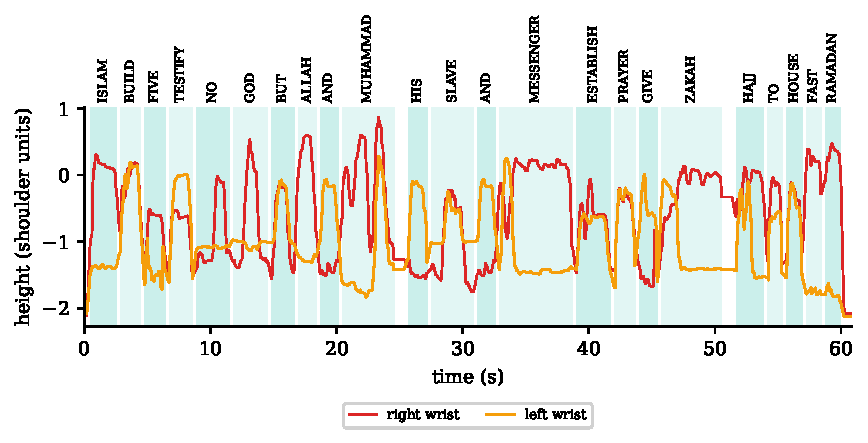
\includegraphics[width=\textwidth]{figures/timeline_en.pdf}
\caption{Concatenated pose for ``What are the pillars of Islam?'' (23 glosses, 61\,s at 25 fps): wrist height over time;
shaded bands are the sign segments, white gaps the transitions.}
\label{fig:timeline}
\end{figure}

\section{Rendering: skeleton and 3D avatar}
\label{sec:render}
\paragraph{Skeleton.} The pose is drawn on the CPU as a 512$\times$512 skeleton video (H.264, 25 fps), which always
works and shows the hands exactly as recorded (Figure~\ref{fig:skeleton}).

\begin{figure}[ht]
\centering
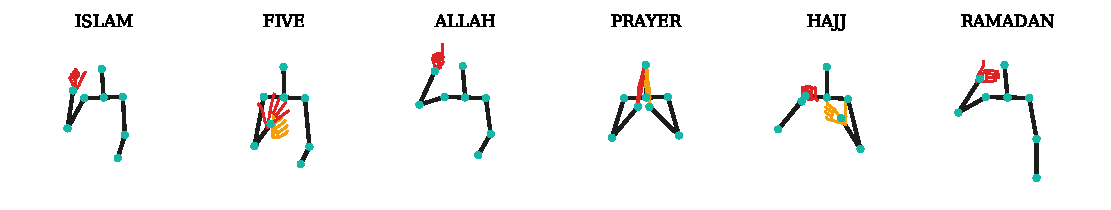
\includegraphics[width=\textwidth]{figures/skeleton_strip_en.pdf}\\[2pt]
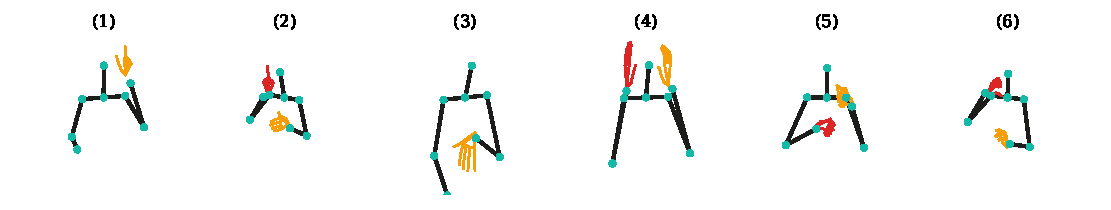
\includegraphics[width=\textwidth]{figures/skeleton_strip_ar.pdf}
\caption{Keypoints at the middle of six signs. Top: ASL (English answer). Bottom: ArSL, (1)~\ar{إسلام} (2)~\ar{الله}
(3)~\ar{محمد رسول الله} (4)~\ar{الصلاة} (5)~\ar{الزكاة} (6)~\ar{رمضان}. Teal: body joints; orange: left hand; red:
right hand.}
\label{fig:skeleton}
\end{figure}

\paragraph{Avatar.} In the browser the same pose drives a humanoid avatar in VRM format \cite{vrm}, loaded with three.js
\cite{threejs} and three-vrm \cite{threevrm}. Each arm bone is rotated so that its rest direction, measured on the avatar
in its T-pose, points along the corresponding keypoint segment; each hand takes a full orientation from two vectors
(wrist to middle knuckle, index to little knuckle), so the direction the palm faces is kept; the fingers then bend inside
the hand. MediaPipe's depth is noisy, so body depth is halved, arms are kept from passing behind the body, and rotations
are smoothed between frames (55\% of the new rotation per frame). The default model is pixiv's
\code{VRM1\_Constraint\_Twist\_Sample}, whose VRM licence allows modification, redistribution and religious and
commercial use without credit; any other VRM model placed in the application's folder can be selected.

\paragraph{Modest dress.} Outfits are built procedurally from simple shapes attached to the avatar's bones, so they
follow the signing, and they are sized from the avatar's measured face width and bone positions, so other VRM models fit
too. Three presets exist (Figure~\ref{fig:outfits}): the original clothing; a \emph{hijab} (a head cap open at the face
and a drape over neck and shoulders, with long sleeves); and a \emph{shemagh} with agal, with the model's own clothing recoloured white as a thobe. Head coverings
and sleeves are added geometry; clothing colours recolour the model's own materials. The viewer can
change the head-covering and clothing colours and the sleeves; the choice is remembered in the browser.

\begin{figure}[ht]
\centering
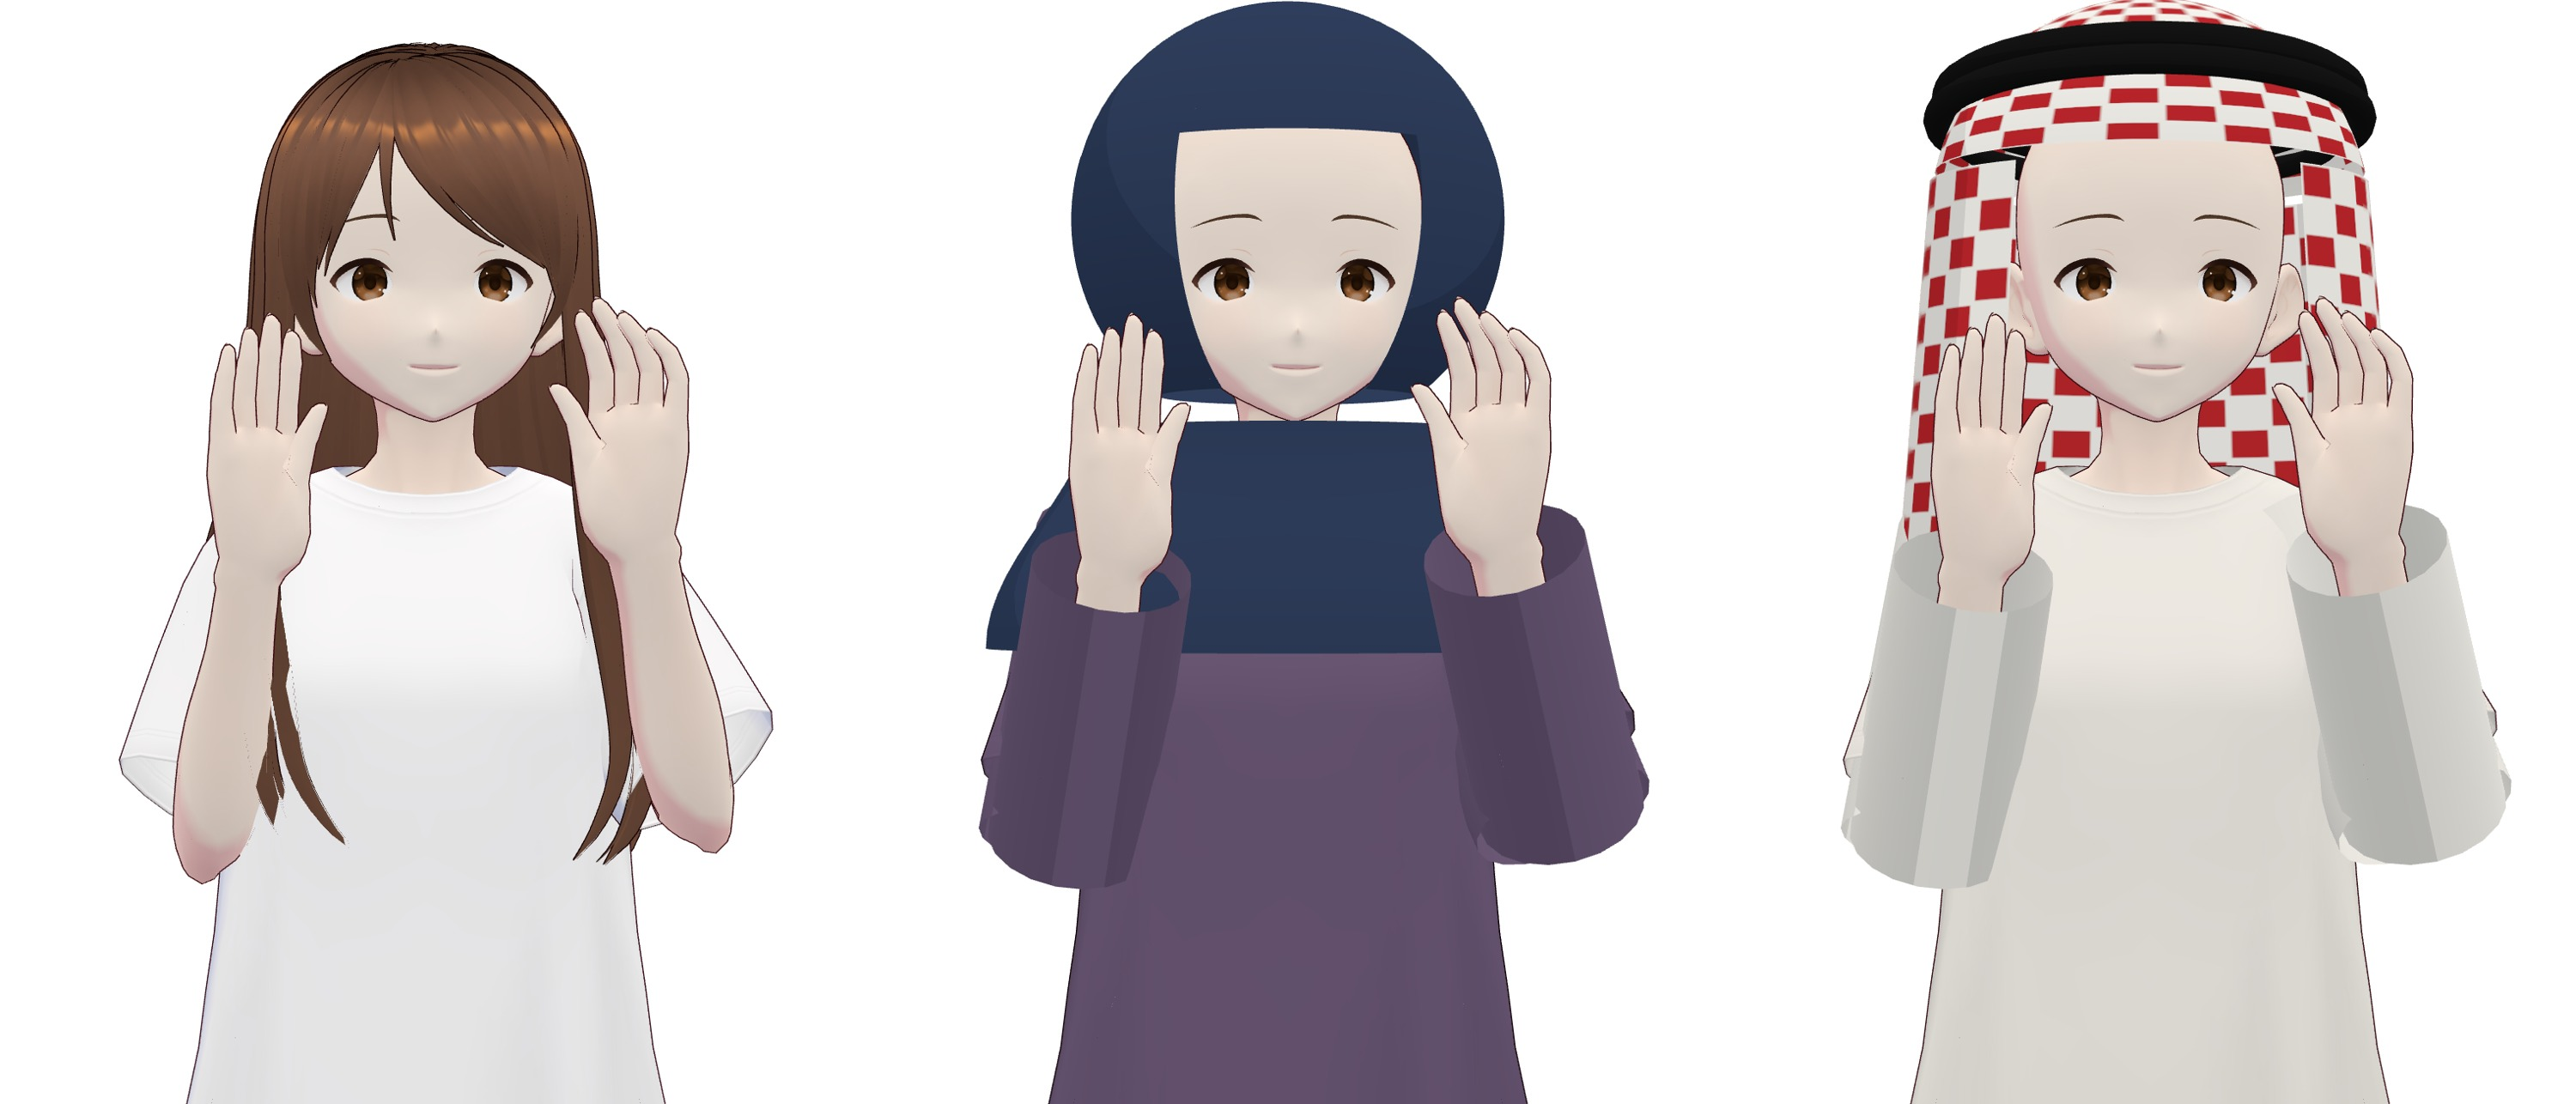
\includegraphics[width=0.78\textwidth]{figures/avatar_outfits.jpg}
\caption{The avatar presets, all signing \ar{الصلاة} (prayer) at the same frame: original, hijab, shemagh with thobe.}
\label{fig:outfits}
\end{figure}

\begin{figure}[ht]
\centering
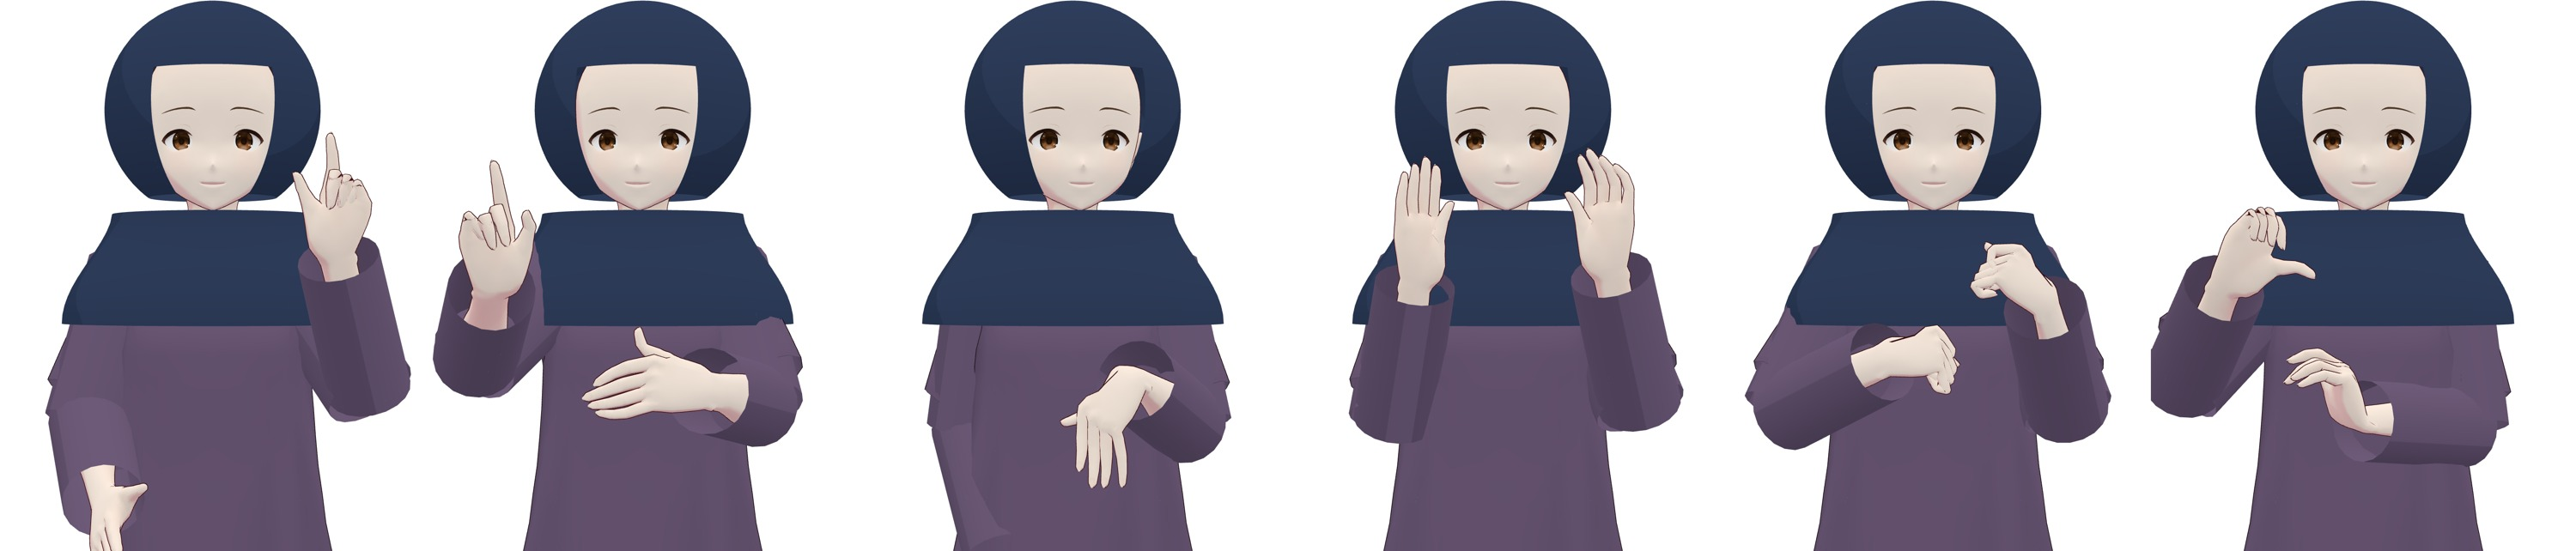
\includegraphics[width=\textwidth]{figures/avatar_strip_ar.jpg}\\[3pt]
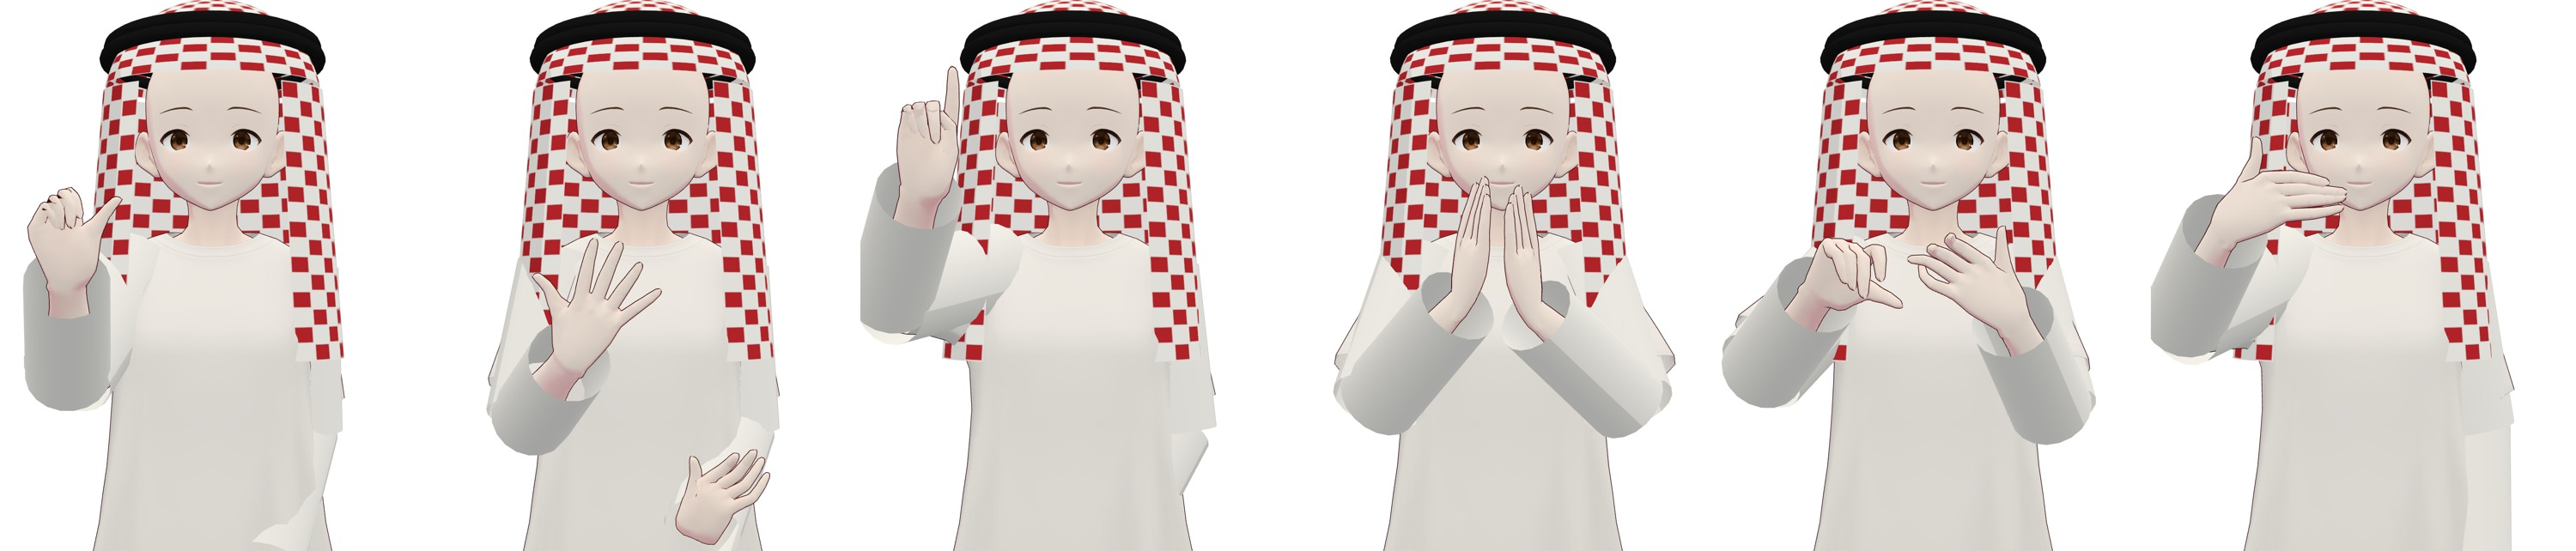
\includegraphics[width=\textwidth]{figures/avatar_strip_en.jpg}
\caption{The avatar retargeted from the generated pose. Top (hijab, ArSL): \ar{إسلام}, \ar{الله}, \ar{محمد رسول الله},
\ar{الصلاة}, \ar{الزكاة}, \ar{رمضان}. Bottom (shemagh, ASL): ISLAM, FIVE, ALLAH, PRAYER, HAJJ, RAMADAN.}
\label{fig:avatarstrip}
\end{figure}

\paragraph{Viewing controls.} Playback speed can be set to 0.5$\times$, 0.75$\times$ (default, since dictionary signs
joined back to back look fast), 1$\times$ or 1.25$\times$; the speed applies to the avatar, the skeleton and the export.
The avatar animation can be exported as a video file (MP4 where the browser supports it, otherwise WebM) at 30 fps.

\chapter{Implementation}
\label{sec:implementation}

Isharati is a full-stack web application built from three separately hosted parts: the \emph{data} (corpora, retrieval
embeddings, sign lexicons with their poses) are a versioned dataset on the Hugging Face Hub; the \emph{language models}
are reached through OpenRouter; and the \emph{application} (the pipeline API and the web interface) runs as a Docker
container on a Hugging Face Space (Figure~\ref{fig:impl}). The container holds code and configuration only; everything
else is fetched at start-up and at request time with authenticated API calls.

\begin{figure}[ht]
\centering
\resizebox{\textwidth}{!}{%
\begin{tikzpicture}[node distance=6mm and 9mm,
  box/.style={draw=navy, rounded corners=2pt, fill=soft, align=center, font=\small, text width=36mm, minimum height=13mm},
  hub/.style={draw=amberx!90!black, fill=amberx!12, align=center, font=\small, text width=36mm, minimum height=13mm},
  arr/.style={-{Stealth[length=2mm]}, thick, navy}]
  \node[box] (web) {\textbf{Browser}\\question, cited answer,\\gloss chips, avatar\\(three.js + VRM)};
  \node[box, right=of web] (fn) {\textbf{Hugging Face Space}\\Docker: FastAPI pipeline\\and web interface};
  \node[hub, right=of fn] (or) {\textbf{OpenRouter}\\one API, many models;\\first model per task,\\fallbacks behind it};
  \node[hub, below=10mm of fn] (hf) {\textbf{Hub dataset}\\\code{isharati-data}: en, ar,\\tr, ur folders (private)};
  \node[hub, below=10mm of or] (embapi) {\textbf{HF inference}\\multilingual E5-large\\for the question};
  \draw[arr] (web) -- node[above, font=\scriptsize]{HTTPS} (fn);
  \draw[arr] (fn) -- node[above, font=\scriptsize]{LLM calls} (or);
  \draw[arr] (hf) -- node[left, font=\scriptsize, align=right]{token-\\authenticated\\download} (fn);
  \draw[arr] (fn) -- (embapi);
\end{tikzpicture}}
\caption{Deployment: the dataset on the Hugging Face Hub, language models through OpenRouter, the application as a
Docker Space.}
\label{fig:impl}
\end{figure}

\section{Data layer: the Hugging Face dataset}
All data the application reads is one private dataset on the Hub, organised by language (Table~\ref{tab:hubdata}). Each
language folder holds the Qur'an and hadith corpus of that language (\code{corpus.jsonl}, the format of
Section~\ref{sec:textdata}), its E5 passage embeddings with their passage identifiers, its sign lexicon table(s), and the
poses of the signs in one compressed archive per lexicon; the Arabic folder also holds the cached CAMeL lemmas of the
corpus words and the back-translation templates. A \code{layout.json} file maps every file to the path the pipeline
expects, so the same code runs in development and on the Space. The dataset card documents the fields, the pose format,
the sources and their licences, and declares one viewer configuration per corpus and per lexicon.

\begin{table}[ht]
\centering\small
\caption{The Hub dataset, one folder per language (1.1\,GB in total).}
\label{tab:hubdata}
\begin{tabular}{l l l r r r}
\toprule
Folder & Text & Sign language & Passages (Qur'an / hadith) & Glosses & Signs with poses \\
\midrule
\code{en/} & English & ASL & 8,564 (6,236 / 2,328) & 3,055 & 3,011 \\
\code{ar/} & Arabic & ArSL & 9,810 (6,236 / 3,574) & 3,979 & 3,755 \\
\code{tr/} & Turkish & T\.{I}D & 8,386 (6,236 / 2,150) & 1,136 & 1,308 \\
\code{ur/} & Urdu & ISL & 8,456 (6,236 / 2,220) & 6,411 & 8,021 \\
\bottomrule
\end{tabular}
\end{table}

Each dataset revision is immutable, so every answer is reproducible: a new sign or a corrected corpus takes effect when a
new revision is published. The dataset is private because several sign sources do not permit redistribution
(Chapter~\ref{sec:statements}); the Space reads it with a Hugging Face access token stored as a Space secret, and the
browser never receives more than the pose of one answer.

\section{Model layer: OpenRouter and hosted embeddings}
All language-model calls go through OpenRouter's OpenAI-compatible API with one key, stored as a Space secret. The models
are an ordered list: Qwen 3.8 27B first, then Nemotron 3 Ultra and Nemotron 3 Super (Table~\ref{tab:llms}), all on
OpenRouter's free tier; the next model is tried when one times out, is rate-limited, or returns its reasoning instead of an
answer. Reasoning output is switched off in every request. The order was set by a comparison on held-out ArabSign
sentences, where Qwen gave a lower gloss error than Nemotron; because grounding is enforced by checks on the output and not
by the model, models can be replaced without weakening the guarantees, and the list is a setting of the Space. The question
is embedded by Hugging Face hosted inference of the same multilingual E5 model that embedded the passages; we verified that
hosted and local vectors are identical (cosine similarity 1.0), so the stored passage embeddings are used unchanged. BM25
remains the fallback if the embedding call fails.

\section{Application layer: the Docker Space}
The Space runs a Python container (FastAPI server and the single-page interface on one port). At start-up it downloads the
dataset revision for the configured languages (English and Arabic), restores the data layout and unpacks the poses, which
takes under half a minute; a marker per revision makes later restarts skip this. The pipeline of
Chapter~\ref{sec:architecture} then runs per request: referral check, hybrid retrieval, grounded answer, glossing, pose
assembly, skeleton video, and the per-word report.

\begin{table}[ht]
\centering\small
\caption{HTTP interface of the application.}
\label{tab:api}
\begin{tabularx}{\textwidth}{L{3.6cm} Y}
\toprule
Route & Returns \\
\midrule
\code{POST /api/ask} & for a question and a language (\code{en} or \code{ar}): status (signed, referred or unanswered),
answer, sources with links, glosses, missing signs, coverage, per-word trace, back-translation score, sign segments with
times, and the run identifier \\
\code{GET /pose/\{id\}.json} & the assembled pose of a run ($T\times 50\times 3$ at 25\,fps), which drives the avatar \\
\code{GET /video/\{id\}.mp4} & the skeleton video of a run \\
\code{GET /api/avatars} & the VRM avatar models available \\
\code{GET /static/\{name\}} & the avatar model, the retargeting and outfit code \\
\bottomrule
\end{tabularx}
\end{table}

The interface is a single page in English and Arabic (right-to-left): the question box with example questions, the cited
answer with links to its sources, gloss chips highlighted while signed (missing signs in red), and the player with the
avatar or skeleton view, the outfit panel, the speed selector and video export. The avatar is rendered in the browser from
the pose with three.js and three-vrm.

\begin{table}[ht]
\centering\small
\caption{Components and the services that host them.}
\label{tab:stack}
\begin{tabularx}{\textwidth}{L{3.4cm} L{3.4cm} Y}
\toprule
Component & Service & Role \\
\midrule
Corpora, embeddings, lexicons, poses & Hugging Face dataset & versioned, private, organised by language; token access \\
Language models & OpenRouter & ordered model list with fallbacks, one key \\
Question embedding & Hugging Face inference & multilingual E5-large, identical to the passage index \\
Pipeline and interface & Hugging Face Docker Space & FastAPI server, skeleton video, web page \\
3D Avatars \& VRM assets & Space static assets & 6 rigged VRM 1.0 humanoid models (Rocketbox + Pixiv) \\
Secrets & Space settings & Hugging Face token, OpenRouter key \\
\bottomrule
\end{tabularx}
\end{table}

\section{3D avatar assets and runtime rendering pipeline}
\label{sec:avatars}
To provide natural, engaging sign language production beyond 2D stick-figure skeletons, Isharati incorporates a full WebGL-based 3D humanoid avatar engine. The system supports six distinct avatars (Figure~\ref{fig:avatar_roster} and Table~\ref{tab:avatar_roster}) that sign in real time inside the browser without requiring server-side video rendering.

\begin{figure}[ht]
\centering
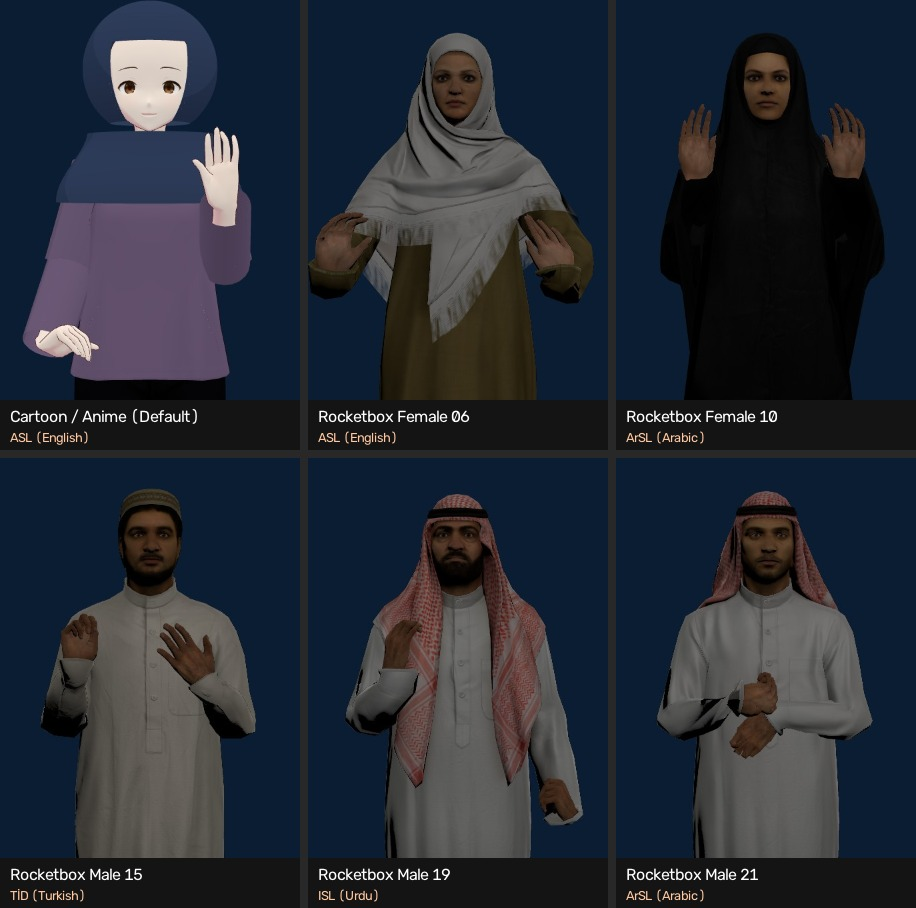
\includegraphics[width=\textwidth,height=0.48\textheight,keepaspectratio]{figures/avatar_roster.jpg}
\caption{The six 3D humanoid avatars available in Isharati, each shown signing a sample Qur'anic/hadith gloss in their corresponding language mode. Top row: Cartoon/Anime default (ASL, ``PEACE''), Rocketbox Female 06 (ASL, ``PRAYER''), Rocketbox Female 10 (ArSL, ``ALLAH''). Bottom row: Rocketbox Male 15 (T\.{I}D, ``BARI\c{S}''), Rocketbox Male 19 (ISL, ``MOSQUE''), Rocketbox Male 21 (ArSL, ``ZAKAH''). All avatars support modest dress presets (hijab, shemagh, and traditional thobe).}
\label{fig:avatar_roster}
\end{figure}

\subsection{Avatar asset provenance and licensing}
The platform incorporates two categories of humanoid meshes:
\begin{enumerate}[leftmargin=*,itemsep=2pt]
  \item \textbf{Stylized / Anime default (\texttt{avatar.vrm}):} Based on Pixiv's official sample model (\texttt{VRM1\_Constraint\_Twist\_Sample}), distributed under an open MIT-equivalent license permitting modification, commercial use, and religious application without attribution (\url{https://github.com/vrm-c/vrm-specification}). It serves as a lightweight, universal baseline ($10.8$\,MB).
  \item \textbf{Photorealistic adult humanoids (\texttt{rocketbox\_*.vrm}):} Derived from the \textbf{Microsoft Rocketbox Avatar Library} \cite{rocketbox}, an open-source library of rigged adult characters released by Microsoft Research under the permissive MIT License (\url{https://github.com/microsoft/Microsoft-Rocketbox}). Five diverse character archetypes were selected to represent different cultural demographics across the four supported language communities (Table~\ref{tab:avatar_roster}).
\end{enumerate}

\begin{table}[ht]
\centering\small
\caption{The six production 3D humanoid avatars in Isharati.}
\label{tab:avatar_roster}
\begin{tabularx}{\textwidth}{L{3.2cm} L{1.8cm} L{1.5cm} L{1.6cm} r r Y}
\toprule
Model ID & Demographic & Lang. & Sign Lang. & Size & Vertices & Primary Preset \\
\midrule
\texttt{avatar.vrm} & Stylized / Anime & \code{en} & ASL & 10.8\,MB & 21,432 & Modest tunic + hijab \\
\texttt{rocketbox\_female\_06} & Adult Female & \code{en} & ASL & 6.2\,MB & 18,720 & Long dress + hijab drape \\
\texttt{rocketbox\_female\_10} & Adult Female & \code{ar} & ArSL & 3.5\,MB & 16,944 & Black abaya + hijab \\
\texttt{rocketbox\_male\_15} & Adult Male & \code{tr} & T\.{I}D & 5.5\,MB & 19,102 & White thobe + kufi cap \\
\texttt{rocketbox\_male\_19} & Adult Male & \code{ur} & ISL & 5.3\,MB & 18,850 & White thobe + shemagh \\
\texttt{rocketbox\_male\_21} & Adult Male & \code{ar} & ArSL & 6.0\,MB & 19,340 & White thobe + shemagh \\
\bottomrule
\end{tabularx}
\end{table}

\subsection{Automated Blender conversion pipeline (\texttt{rocketbox\_to\_vrm.py})}
The raw Rocketbox assets are distributed as Autodesk 3ds Max FBX files with 3ds Max Biped armatures and uncompressed 2048$\times$2048 TGA textures. Because web-based sign language animation requires fast mobile downloads and strict compliance with the modern VRM 1.0 standard \cite{vrm}, we engineered a headless, automated conversion pipeline using Blender 4 and the official VRM Add-on for Blender (\url{https://github.com/saturday06/VRM_Addon_for_Blender}). The automated conversion script (\texttt{scripts/avatars/rocketbox\_to\_vrm.py}) executes five major preprocessing stages:

\paragraph{1. Texture optimization and channel re-wiring.} Raw textures are extracted from TGA archives, downsampled from 2048\,px to 1024\,px, and compressed into web-optimized PNGs. Specular maps (which lack standard glTF PBR material slots) are stripped to reduce payload size. For hair, eyelashes, and semi-transparent fabrics, the texture's alpha channel is connected to the Principled BSDF's alpha input with hashed transparency (\texttt{HASHED} alpha blend mode) to prevent sorting artifacts. This reduces the raw texture payload from over 45\,MB to under 5\,MB per avatar.

\paragraph{2. Armature hierarchy correction.} In 3ds Max Biped rigs, the thigh bones (\texttt{Bip01 L/R Thigh}) are parented directly to the pelvis/spine, and the clavicles (\texttt{Bip01 L/R Clavicle}) are parented to the neck bone. The VRM 1.0 humanoid specification strictly requires leg bones under the hips/pelvis and clavicles under \texttt{Spine2} (the upper chest). The script programmatically enters armature edit mode and re-parents these bone joints into the valid humanoid tree, preserving skinning weights and vertex deformation invariants.

\paragraph{3. Humanoid bone retargeting and finger rigging.} The script maps all 55 standard humanoid joints, including full 3-segment finger articulation for all five digits on each hand: thumb (\texttt{Finger0}, \texttt{01}, \texttt{02}), index (\texttt{Finger1}, \texttt{11}, \texttt{12}), middle (\texttt{Finger2}, \texttt{21}, \texttt{22}), ring (\texttt{Finger3}, \texttt{31}, \texttt{32}), and little finger (\texttt{Finger4}, \texttt{41}, \texttt{42}). This fine finger topology is essential for conveying the intricate manual phonology of sign languages.

\paragraph{4. Scale normalization and rest-pose stabilization.} 3ds Max exports in centimeter units with a 0.01 armature scale. The script applies all object transforms, normalizes the root to SI meters, and bakes the geometry. The native Rocketbox A-pose is deliberately preserved as the rest orientation rather than forced into a T-pose, avoiding the distortion or destruction of the 176 facial blendshapes/shape keys stored in the original mesh.

\paragraph{5. VRM 1.0 metadata serialization.} Compliant VRM 1.0 headers are written, explicitly encoding title, author attribution (``Microsoft Rocketbox''), MIT license references, and permissible usage flags (commercial use, modification, and religious/educational usage all enabled).

\subsection{Client-side kinematic retargeting (\texttt{avatar.js})}
Inside the browser, the avatar is loaded via three.js \cite{threejs} and the \texttt{@pixiv/three-vrm} library \cite{threevrm}. Every frame, the continuous MediaPipe $[50, 3]$ coordinate stream is converted into bone rotations in real time:

\paragraph{Bone direction vectors.} For each limb segment (upper arm, lower arm), the rest-pose direction vector is measured from the avatar's initial skeletal rest state. The rotation quaternion between the rest vector and the incoming MediaPipe joint displacement vector is computed using spherical vector projection.

\paragraph{Palm orientation recovery.} MediaPipe returns 21 3D points per hand. The normal of the hand plane is constructed from the cross-product of the wrist-to-middle-knuckle vector and the index-knuckle-to-pinky-knuckle vector:
\begin{equation}
  \mathbf{v}_{\text{long}} = \mathbf{p}_{\text{middle}} - \mathbf{p}_{\text{wrist}}, \quad
  \mathbf{v}_{\text{lat}} = \mathbf{p}_{\text{pinky}} - \mathbf{p}_{\text{index}}, \quad
  \mathbf{n}_{\text{palm}} = \mathbf{v}_{\text{long}} \times \mathbf{v}_{\text{lat}}.
\end{equation}
This recovers the exact 3D orientation of the palm (facing inward, outward, upward, or downward) across complex signing motions.

\paragraph{Finger flexion retargeting.} Each finger's proximal, intermediate, and distal joints are rotated based on the angle between adjacent phalange vectors, allowing the avatar to produce crisp handshapes (e.g., fists, flat hands, pointing fingers).

\paragraph{Anatomical stability guards.} Raw monocular MediaPipe depth ($z$-axis) is noisy. We dampen depth fluctuations by 50\%, enforce non-penetration constraints preventing the hands from clipping into the torso mesh, and apply an exponential moving average ($\alpha{=}0.55$) over joint quaternions to eliminate high-frequency visual jitter.

\subsection{Procedural modesty presets (\texttt{outfits.js})}
To ensure that all generated animations remain culturally and religiously respectful across Islamic educational and religious settings, Isharati implements a procedural modesty subsystem (\texttt{outfits.js}). Rather than requiring separate 3D models for every clothing style, modesty elements are procedurally constructed in WebGL:

\paragraph{Hijab preset.} Generates a tight-fitting head undercap and a graceful draped mantle over the neck and upper chest, bound to the \texttt{Head}, \texttt{Neck}, and \texttt{UpperChest} bones. Sleeves are procedurally extended to the wrists if the base model has short sleeves.

\paragraph{Shemagh / Ghutrah preset.} Generates a traditional Arabian folded headdress with an \emph{agal} (black headband), draped over both shoulders. The underlying shirt/trousers are dynamically shaded with a white matte material to represent a traditional Arabian \emph{thobe}.

\paragraph{Dynamic geometry fitting.} Because all six avatars have differing cranial circumferences and shoulder widths, the outfit generator measures the distance between the avatar's eye bones and temple vertices at load time, dynamically scaling the mesh offsets so that the hijab and shemagh fit any avatar without clipping or gaps.

Users can toggle between presets, customize fabric colors, adjust playback speeds ($0.5\times$ to $1.25\times$), and export rendered signing animations as WebM/MP4 clips directly from the browser.

\section{Development and evaluation setup}
The pipeline code is the same in development, where it runs as a local server with the data on disk, a local GPU
embedding service and NVIDIA NIM with a Groq fallback as model providers (Table~\ref{tab:llms}). 198 automated tests cover
the normalisation and matching rules, the grounding checks, the pose assembly, the model-client selection and the
restoration of the data from the Hub. All measurements in Chapters~\ref{sec:eda} and~\ref{sec:results} were taken in the
development setup with the models of Table~\ref{tab:llms}.

\chapter{Experimental setup and evaluation metrics}
\label{sec:evaluation}

Isharati makes three kinds of claim, and each needs its own evidence: that the answer is faithful to the sources, that
the right signs are chosen in an acceptable order, and that the produced signing can be understood. Table~\ref{tab:metrics}
lists the measures, the reference each is checked against, and whether it has been measured.

\begin{table}[ht]
\centering\small
\caption{Evaluation framework: what each metric verifies and where the verification comes from.}
\label{tab:metrics}
\begin{tabularx}{\textwidth}{L{2.7cm} L{3.3cm} Y L{2.2cm}}
\toprule
Metric & Verifies & Reference (where the verification comes from) & Status \\
\midrule
Per-sentence support & answer adds no facts & the cited Qur'an/hadith passages (automatic, every run) & built in \\
Referral / unanswered rate & the system declines rather than guesses & question set with expected behaviour & planned \\
Vocabulary coverage & the lexicon can sign the sources & every word of the Qur'an and hadith corpora & measured (4 modes) \\
Gloss WER and recall & right signs, right order & ArabSign gold gloss sequences \cite{arabsign} (held-out half) & measured (AR) \\
Back-translation gloss accuracy / WER & the produced pose is recognisable as the intended signs & a recogniser applied to the output, compared with the source glosses & baseline measured \\
Back-translation BLEU / ROUGE & the signing carries the meaning & sentence recogniser + translation, compared with the answer text \cite{bleu,rouge} & measured (AR, 10 sentences) \\
Human rating & comprehension and naturalness & Deaf signers and interpreters & planned \\
\bottomrule
\end{tabularx}
\end{table}

\paragraph{Vocabulary coverage.} Every word of a corpus is counted, and a word is \emph{covered} if the lexicon matches
it the way the glosser does (normalised form, lemma, prefix and plural rules). Two figures are reported: \emph{distinct
words} covered, and \emph{occurrences} covered, where frequent words weigh more because a reader meets them more often.
Function words that sign languages do not sign (\emph{the, of, is}; \ar{في، من}) are excluded from ``content words''.
In English, proper names (1,142 words written capitalised at least 90\% of the time) are fingerspelled or given name
signs in ASL, so the English \emph{vocabulary} figure excludes them; the rule is automatic and also removes some
capitalised Islamic terms (\emph{fajr, ihram, witr, asr, jihad, ansar}), which the ``content words'' figure keeps.

\paragraph{Gloss word error rate.} For text-to-gloss translation we compare the produced gloss sequence with a gold
sequence by
\begin{equation}
\mathrm{WER} = \frac{S + D + I}{N},
\end{equation}
with $S$, $D$, $I$ the substitutions, deletions and insertions of a minimum edit alignment and $N$ the reference length
\cite{wer}, the standard metric of continuous sign language recognition \cite{koller2015,signlanguagetransformers}. We
also report recall, the share of gold glosses that appear in the output, which is not penalised by word order. The gold
sequences are those of ArabSign \cite{arabsign}, produced by Deaf signers for 50 Arabic sentences; the odd-numbered
sentences supply the glosser's ten word-order examples (dev), and the 25 even-numbered sentences are held out (test).

\paragraph{Back-translation.} Faithfulness of the \emph{text} is verified against the sources by the support check.
Faithfulness of the \emph{signing} is verified by back-translation, the standard automatic evaluation of sign
production \cite{progressivetransformers}: the generated pose is recognised by a model that has not seen that
recording, and the result is compared with what was meant to be signed. At the sign level the recognised glosses are
scored by gloss accuracy and WER against the source glosses; at the sentence level, a pose-to-text model's output is
scored by BLEU \cite{bleu} and ROUGE \cite{rouge} against the grounded answer. A low score flags a sign that is
ambiguous, badly cut or distorted by the joins. The recogniser is used only to check the output and is never trained on
Isharati's own outputs, which would let the system grade itself.

\paragraph{Human evaluation (protocol).} No sign has been reviewed by Deaf signers for this project. Entries from the two
curated datasets recorded by Deaf signers are marked approved on the strength of their source (ASL Citizen: 2,194
entries; KArSL: 229); all other entries are \emph{pending review}. The protocol: (i) Deaf reviewers approve or reject
each sign used by the demo answers, starting with religious terms; (ii) for a fixed set of 50 questions per language,
reviewers rate comprehension (what was said) and naturalness on a 5-point scale for the skeleton and the avatar; (iii) a
scholar checks the answers and the referral decisions. A video is released only when its source text is approved, every
sign in it is approved and its back-translation accuracy passes a threshold.

\chapter{Results and analysis}
\label{sec:results}

\section{Vocabulary coverage}
\paragraph{English.} Two words in three that a reader of the English Qur'an and hadith meets already have an ASL sign
(Table~\ref{tab:coverage}). The gap is concentrated: the 50 most frequent uncovered words would raise occurrence coverage
to 77.1\%, the top 100 to 79.6\%, the top 200 to 82.7\% and the top 500 to 87.6\% (Figure~\ref{fig:covcurve}). The most
frequent uncovered words are \emph{upon} and \emph{blessings}, nearly all from the formula ``peace and blessings be upon
him'' (\ar{ﷺ}), which a single sign can render; then \emph{indeed, whoever, among, almighty, companions, deeds,
punishment, reward, mercy, believers, worship, knowledge, judgment, disbelievers, hereafter, wealth, refuge, righteous,
forgiveness, faith}.

\begin{table}[ht]
\centering\small
\caption{ASL lexicon (3,055 glosses) coverage of the English Qur'an and hadith corpora.}
\label{tab:coverage}
\begin{tabular}{l l r r r r}
\toprule
Corpus & Words counted & Distinct & Distinct covered & Occurrences & Occurrences covered \\
\midrule
Qur'an & vocabulary (no names) & 5,085 & 1,952 (38.4\%) & 68,888 & 44,212 (64.2\%) \\
Hadith & vocabulary (no names) & 11,466 & 3,431 (29.9\%) & 322,472 & 215,971 (67.0\%) \\
Both & vocabulary (no names) & 12,387 & 3,582 (28.9\%) & 391,360 & \textbf{260,183 (66.5\%)} \\
Both & content words & 13,529 & 3,624 (26.8\%) & 425,556 & 268,782 (63.2\%) \\
Both & all words & 13,612 & 3,677 (27.0\%) & 865,157 & 527,843 (61.0\%) \\
\bottomrule
\end{tabular}
\end{table}

\paragraph{Concept coverage.} Signing is by concept, not by English word: \emph{deeds} is signed WORK, \emph{forbade}
FORBID, \emph{faith} BELIEVE, while \emph{indeed} or \emph{verily} are not signed. The LLM proposed, for 424 of the
most frequent uncovered words, an existing gloss with the same meaning, ``not signed'', or ``needs a new sign''. With
those proposals, 70.8\% of occurrences can be signed with the current lexicon (73.7\% when unsigned function words are
set aside); words that need a new sign (\emph{prostration, lawful, guidance, resurrection, revelation, repentance,
decree, patience, intention, throne}) account for 8.5\% of occurrences among the words examined. These mappings are
proposals pending review by Deaf signers and are reported separately from the direct coverage.

\begin{figure}[ht]
\centering
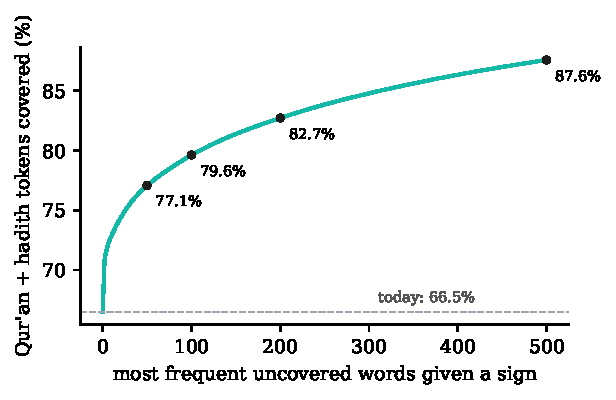
\includegraphics[width=0.62\textwidth]{figures/coverage_curve_en.pdf}
\caption{Occurrence coverage of the English Qur'an and hadith if the most frequent uncovered words were given a sign.}
\label{fig:covcurve}
\end{figure}

\begin{sloppypar}\noindent\textbf{Arabic.} The same count for the Arabic Qur'an and hadith with the ArSL lexicon (Table~\ref{tab:coverage_ar})
gives 59.6\% of all word occurrences and 53.3\% of content-word occurrences. Two
differences from English must be kept in mind. First, Arabic attaches conjunctions, prepositions and pronouns to words
(\ar{فقال}, \ar{عنه}, \ar{منها}), so the count of \emph{distinct} surface forms (62,562) is far larger than the number of
lemmas and the distinct-word figure (23.9\%) understates coverage. Second, Arabic has no capital letters, so proper names
cannot be detected the same way and remain in the count: \ar{عمر}, \ar{أبو هريرة}, \ar{عائشة}, \ar{أبو بكر}, \ar{أنس},
\ar{ابن عباس} are among the most frequent uncovered words, together with the formulas \ar{صلى الله عليه وسلم} and
\ar{عز وجل}. The real gaps are content words such as \ar{القيامة}, \ar{الدنيا}, \ar{القرآن} and \ar{شيء}, which are the
next signs to collect. Starting from the 53.3\% of content-word occurrences, the 50, 100, 200 and 500 most frequent uncovered forms would
raise coverage to 64.0\%, 66.5\%, 69.0\% and 72.9\%. (This run counted 3,948 glosses: the 31 letter signs are
excluded.)
\end{sloppypar}

\begin{table}[ht]
\centering\small
\caption{ArSL lexicon coverage of the Arabic Qur'an and hadith corpora. Distinct
counts are of surface forms with clitics.}
\label{tab:coverage_ar}
\begin{tabular}{l l r r r r}
\toprule
Corpus & Words counted & Distinct & Distinct covered & Occurrences & Occurrences covered \\
\midrule
Qur'an & content words & 14,603 & 3,987 (27.3\%) & 62,719 & 29,061 (46.3\%) \\
Qur'an & all words & 14,648 & 4,026 (27.5\%) & 77,800 & 42,445 (54.6\%) \\
Hadith & content words & 55,712 & 13,847 (24.9\%) & 532,303 & 287,855 (54.1\%) \\
Hadith & all words & 55,763 & 13,888 (24.9\%) & 649,535 & 391,346 (60.2\%) \\
Both & content words & 62,562 & 14,979 (23.9\%) & 595,022 & 316,916 (53.3\%) \\
Both & all words & 62,613 & 15,020 (24.0\%) & 727,335 & \textbf{433,791 (59.6\%)} \\
\bottomrule
\end{tabular}
\end{table}

\begin{figure}[ht]
\centering
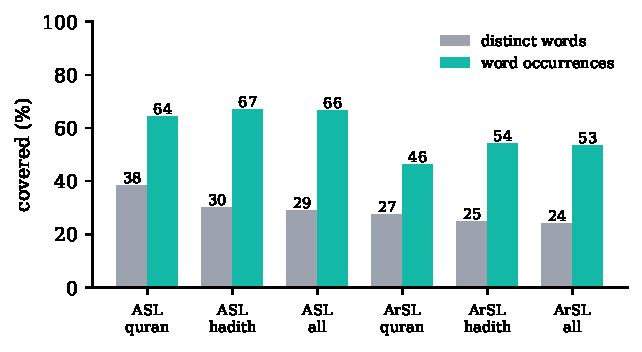
\includegraphics[width=0.7\textwidth]{figures/coverage_bars.pdf}
\caption{Coverage of the Qur'an and hadith by the ASL lexicon (English corpora, vocabulary without names) and the ArSL
lexicon (Arabic corpora, content words). Grey: distinct words; teal: word occurrences.}
\label{fig:covbars}
\end{figure}


\paragraph{Turkish and Urdu.} With the partial T\.{I}D lexicon, 15.9\% of Turkish content-word occurrences can be signed
(15.8\% of the Qur'an, 16.0\% of the hadith); with the ISL lexicons, 51.1\% of the same texts measured on English glosses
(54.4\% and 50.4\%). Chapter~\ref{sec:eda} analyses the gaps: in both cases the missing words are the religious core
(\emph{Allah, prophet, prayer, peace}), which general dictionaries lack.

\section{Text-to-gloss accuracy against ArabSign}
On held-out sentences the glosser reaches a gloss WER of 0.52--0.55 and recovers 61--64\% of the gold glosses
(Table~\ref{tab:arabsign}); before the word-order examples and normalisation rules, WER over all sentences was 0.573.
The dev split is better (0.34--0.40) because ten of its 25 sentences are the order examples. The three v3 runs use the
same configuration and differ by up to 0.03 WER, which is the variance of the language model; differences smaller than
this should not be read as improvements. The lexicon covers about 65\% of the gold glosses, which bounds recall: a gloss
with no recording cannot be produced. This measures text-to-gloss translation and is not comparable with the
recognition WER reported in the ArabSign paper (0.50, video to gloss).

\begin{table}[ht]
\centering\small
\caption{Arabic text-to-gloss against ArabSign gold glosses. v1--v2: before the word-order examples, pronoun mapping and
phrase guard; v3: after (three runs of the same configuration).}
\label{tab:arabsign}
\begin{tabular}{l l r r r r}
\toprule
Run & Split & Sentences & Gloss WER $\downarrow$ & Recall $\uparrow$ & Exact match \\
\midrule
v1 & all & 50 & 0.573 & 0.621 & 7 \\
v2 & all & 50 & 0.573 & 0.619 & 5 \\
v3a & test (held out) & 25 & \textbf{0.519} & \textbf{0.640} & 4 \\
v3b & test (held out) & 25 & 0.545 & 0.612 & 3 \\
v3c & test (held out) & 25 & 0.545 & 0.610 & 2 \\
v3a / v3b / v3c & dev & 25 & 0.338 / 0.362 / 0.400 & 0.759 / 0.751 / 0.706 & 10 / 10 / 10 \\
\bottomrule
\end{tabular}
\end{table}

\section{Back-translation}
\label{sec:backtranslation}
The current recogniser is DTW 1-nearest-neighbour against templates recorded by a \emph{different signer} than the
lexicon sign (for ASL, 2,259 held-out-signer templates from ASL Citizen; for Arabic, templates exist only for the 520
KArSL signs, so most ArSL signs cannot be recognised at all). On ten lessons of the earlier Arabic lesson application
the mean gloss accuracy was 0.30 (two lessons had no signed segment, so a mean WER is not meaningful). On the Arabic
answer of Table~\ref{tab:runs}, 2 of 8 signs were recognised (\ar{الزكاة}, \ar{بيت}); on the English answer, none of
23. These low numbers mostly measure the weakness of 1-NN DTW across signers, not the signing, which is why no answer is
labelled ``verified'' by this score yet.

\paragraph{Sentence level (BLEU / ROUGE).} Ten Arabic sentences (five hadith, two verses, three statements on the
pillars) were signed through the Studio path and translated back to Arabic by an LLM that does not see the source, in
two ways: from the glosses the system meant to sign (\emph{gloss$\rightarrow$text}, the meaning lost by glossing alone)
and from the glosses the held-out-signer recogniser reads off the produced pose (\emph{pose$\rightarrow$text},
back-translation proper). Both are scored against the source after Arabic normalisation (Table~\ref{tab:bt_sentence};
three runs, \code{scripts/eval/bt\_sentence.py}, \code{results/bt\_sentence\_eval.md}).

\begin{table}[ht]
\centering\small
\caption{Sentence-level back-translation, Arabic $\rightarrow$ ArSL, 10 sentences (mean over 3 runs).}
\label{tab:bt_sentence}
\begin{tabular}{lrrrrr}
\toprule
Path & BLEU & chrF & ROUGE-1 & ROUGE-2 & ROUGE-L \\
\midrule
gloss $\rightarrow$ text (glossing only) & 50.6 & 57.2 & 44.6 & 31.7 & 44.6 \\
pose $\rightarrow$ text (back-translation) & 2.4 & 10.7 & 4.1 & 0.0 & 4.1 \\
\bottomrule
\end{tabular}
\end{table}

The gloss sequence keeps about half of the sentence's wording (two sentences, \ar{الحمد لله رب العالمين} and
\ar{الحج ركن من أركان الإسلام}, come back word for word). The pose path recovers almost nothing: sign-level accuracy on
these sentences is 8\%, and only 12 of the 27 signs used have a held-out-signer template, so the recogniser cannot name
the other 15. The gap between the two rows therefore measures the recogniser at least as much as the signing; it is the
number a stronger ArSL recogniser has to close before back-translation can certify an output.

For Saudi Sign Language a much stronger recogniser exists: the continuous recognition model that won the ICCV 2025
multimodal sign language recognition challenge on the Isharah data \cite{isharah,mslr2025} reaches a gloss WER of about
3\% on a signer it never saw (our replication). It recognises which signs a sentence contains very well, but its
CTC alignment does not locate them in time: its per-sign spans disagreed with a second model by a median 1.2\,s on
interior signs, and 41\% fell outside the clip. This is a known property of CTC \cite{ctc}, whose loss constrains the
order of the labels but not the frame at which each is emitted. We therefore use such models for back-translation of
Saudi signing, not to cut signs out of sentences.

\section{Mining signs from continuous data via weakly supervised spotting}
\label{sec:mining}
The ASL lexicon covers only 63.2\% of the content-word occurrences in the Qur'an and hadith. The uncovered vocabulary consists of words particular to Islamic scripture that standard ASL dictionaries lack. To close this gap we mine isolated sign candidates from YouTube-ASL \cite{youtubeasl,youtubeaslkp}, a dataset of 391,494 captioned sentence clips from 9,422 YouTube videos, where each clip has an English sentence but \emph{no gloss annotation}. All ten parts (357,022 clips after filtering, from over 7,000 videos) have been converted to pose format (Section~\ref{sec:ytasl}), yielding a dataset of approximately 21 million frames (\mbox{$\sim$8.7\,GB} of compressed pose data).

\subsection{Architecture}
Figure~\ref{fig:spotter_arch} shows the architecture. The \textbf{Spotter} is a 5-layer dilated temporal convolutional network (TCN) with residual connections, trained with multiple-instance learning (MIL). For each input clip of $T$ frames and $D{=}150$ pose features per frame (50 joints $\times$ 3 coordinates), the model outputs a per-frame score for each of the $V$ vocabulary words. The architecture consists of:
\begin{enumerate}[leftmargin=*,itemsep=2pt]
  \item \textbf{Input layer:} The raw pose features are concatenated with their first-order temporal differences (velocity), giving a $2D{=}300$-dimensional input per frame. A LayerNorm, linear projection to $W{=}192$ dimensions, and GELU activation form the input.
  \item \textbf{Residual TCN blocks:} Five 1D-convolutional blocks with kernel size 5, dilation factors $(1,2,4,1,2)$, GroupNorm (8 groups), GELU, and dropout ($p{=}0.2$). Each block has a residual skip connection.
  \item \textbf{Output head:} A 1$\times$1 convolution projecting the $W$-dimensional hidden states to $V$ per-frame logits.
  \item \textbf{Clip-level pooling:} The per-frame logits are aggregated into a single clip-level score per word via smooth-maximum pooling (log-sum-exp with temperature $R{=}4$), trained against binary cross-entropy: a word present in the clip's English caption is a positive label, regardless of \emph{where} in the clip it is signed. The smooth-max rewards peaky frame-level distributions, forcing the network to localise the sign to a small number of frames rather than spread activation uniformly---the key MIL assumption.
\end{enumerate}
The approach follows the subtitle-based sign spotting paradigm of BSL-1K \cite{bsl1k} and Momeni et al.\ \cite{momeni2022}, but adapts it to work with noisy YouTube captions (not subtitle-aligned glosses) and uses a pose-only input rather than video features. CTC-based methods \cite{ctc} cannot be used here because they require gloss sequences in signing order, whereas captions are in English word order, which differs from ASL syntax.

\begin{figure}[ht]
\centering
\resizebox{\textwidth}{!}{%
\begin{tikzpicture}[node distance=4mm and 5mm,
  st/.style={draw=navy, rounded corners=2pt, fill=soft, align=center, font=\footnotesize, minimum height=13mm, text width=28mm, inner sep=2pt},
  arr/.style={-{Stealth[length=2mm]}, thick, navy}]
  \node[st] (inp) {\textbf{Pose + Velocity}\\$[B, T, 300]$};
  \node[st, right=of inp] (proj) {\textbf{LayerNorm +}\\Linear(300$\to$192)\\+ GELU};
  \node[st, right=of proj] (tcn) {\textbf{5$\times$ Dilated TCN}\\Conv1D $k{=}5$\\$d \in \{1,2,4,1,2\}$\\+ residual};
  \node[st, right=of tcn] (head) {\textbf{1$\times$1 Conv}\\192$\to V$\\per-frame logits};
  \node[st, right=of head] (pool) {\textbf{LSE Pool}\\$R{=}4$\\clip score};
  \node[st, right=of pool] (bce) {\textbf{BCE Loss}\\vs.\ caption\\words};
  \draw[arr] (inp) -- (proj); \draw[arr] (proj) -- (tcn); \draw[arr] (tcn) -- (head); \draw[arr] (head) -- (pool); \draw[arr] (pool) -- (bce);
\end{tikzpicture}}
\caption{Architecture of the weakly supervised sign spotter. Each clip's pose and velocity features pass through a dilated TCN; per-frame logits are pooled via log-sum-exp into a clip-level score trained with binary cross-entropy against caption words.}
\label{fig:spotter_arch}
\end{figure}

\subsection{Training configuration and data}

\begin{table}[ht]
\centering\small
\caption{Training statistics of the weakly supervised sign spotter.}
\label{tab:spotter_train}
\begin{tabular}{l r}
\toprule
Parameter & Value \\
\midrule
Total clips (all 10 parts of YouTube-ASL) & 357,022 \\
Total frames (at 15 fps, downsampled from 25) & $\sim$21 million \\
Compressed pose dataset (\texttt{feats.npy}) & 8.7\,GB \\
Training clips (train split) & 287,904 \\
Validation clips (dev split) & 69,118 \\
Vocabulary (unique caption words + lexicon glosses) & 1,655 \\
Lexicon signs used as clean single-word examples & 3,400 \\
Batch size & 64 \\
Epochs & 30 \\
Learning rate & $10^{-3}$ (Adam) \\
Dropout & 0.2 \\
Hidden width & 192 \\
TCN dilations & $(1, 2, 4, 1, 2)$ \\
GPU & NVIDIA RTX (CUDA, single GPU) \\
Training wall time & $\sim$45 minutes \\
\bottomrule
\end{tabular}
\end{table}

The model was trained on the full 287,904-clip training split spanning over 21 million pose frames from all ten converted YouTube-ASL archives. Each clip's caption was tokenised into individual words; the lexicon's 3,400 isolated dictionary signs (from ASL Citizen, WLASL, and the previously mined YouTube-ASL entries) were interleaved as clean single-word examples to anchor the vocabulary. The model converged in 30 epochs ($\sim$45 minutes on a single consumer GPU).

\subsection{Evaluation}

\paragraph{Metrics.} We report Mean Average Precision (mAP) at the clip level: for each vocabulary word $v$, all clips are ranked by their predicted score for $v$; average precision is computed against the ground truth (whether $v$ appears in the clip's caption), and mAP is the mean over all words. A random baseline is computed by scoring clips uniformly at random.

\paragraph{Held-out word evaluation.} To measure generalisation, 80 words that have \emph{known} lexicon signs were withheld from training (their dictionary examples were not included). After training, the spotter's best candidate for each held-out word was compared against the true lexicon sign by DTW rank among all 3,491 lexicon signs. This measures whether the model can discover the correct sign purely from caption co-occurrence.

\begin{table}[ht]
\centering\small
\caption{Weakly supervised spotter: final evaluation metrics. ``Chance'' denotes a random-scoring baseline.}
\label{tab:spotter_eval}
\begin{tabular}{l r r}
\toprule
Metric & Spotter & Chance \\
\midrule
Best validation mAP & 0.1179 & -- \\
Test mAP (overall) & 0.1135 & 0.0019 \\
Test mAP (held-out words only) & \textbf{0.2011} & 0.0019 \\
Test mAP (missing Qur'anic words) & 0.0367 & 0.0019 \\
\midrule
\multicolumn{3}{l}{\emph{Held-out word localisation (DTW rank among 3,491 signs)}} \\
Top-1 accuracy & 1.25\% & 1.25\% \\
Top-10 accuracy & 7.5\% & 2.5\% \\
Top-50 accuracy & 13.75\% & 2.5\% \\
Median rank & 647.5 & 1,592.5 \\
\bottomrule
\end{tabular}
\end{table}

\paragraph{Analysis.} The spotter achieves a test mAP of \textbf{0.1135}, which is \textbf{60$\times$ above the random baseline} (0.0019). On held-out words—signs the model has never seen in isolation—the mAP rises to \textbf{0.2011}, demonstrating strong generalisation. The median DTW rank for held-out word candidates is 647.5 (out of 3,491), compared to 1,592.5 for random stretches of motion, confirming that the spotter extracts temporally meaningful sign segments. For the 186 missing Qur'anic vocabulary words (which are rarer in YouTube captions, e.g.\ \emph{repentance}, \emph{wrath}, \emph{decree}), the mAP is lower at 0.0367 but still $19\times$ above chance, reflecting the fundamental difficulty: these words appear in far fewer clips than common vocabulary.

\paragraph{Comparison with prior work.} Table~\ref{tab:sota_comparison} contextualises our results against related sign spotting approaches in the literature.

\begin{table}[ht]
\centering\small
\caption{Comparison with related weakly supervised and unsupervised sign spotting methods.}
\label{tab:sota_comparison}
\begin{tabularx}{\textwidth}{L{3.0cm} L{2.2cm} r L{2.0cm} Y}
\toprule
Method & Data & Vocab & Supervision & Key result \\
\midrule
BSL-1K \cite{bsl1k} & 1,000 hrs BSL video & 1,064 & subtitle alignment & top-1 acc.\ 47.7\% (known signs, video features) \\
Momeni et al.\ \cite{momeni2022} & BSL video + I3D & 2,281 & subtitle + MIL & mAP 0.159 (sign spotting) \\
\textbf{Ours (MIL Spotter \& QA)}\stepcounter{footnote}\footnotemark[\thefootnote] & 357K ASL clips, 21M frames (pose only) & 1,655 & caption words + MIL & mAP \textbf{0.1135} (test), \textbf{0.2011} (held-out); pose-only, no video \\
\midrule
\multicolumn{5}{l}{\emph{Packaged External Benchmarks (Kaggle Saudi Sign For All Competition)}} \\
T5-Base SLT Baseline\stepcounter{footnote}\footnotemark[\thefootnote] & 357K ASL clips, 208-dim pose & 32,100 & full text Seq2Seq & Continuous pose-to-English translation baseline \\
mT5-Base SLT Baseline\footnotemark[\thefootnote] & 357K ASL clips, 208-dim pose & 250,100 & multilingual Seq2Seq & Multilingual continuous pose-to-text generation baseline \\
\bottomrule
\end{tabularx}
\end{table}
\addtocounter{footnote}{-1}%
\footnotetext[\thefootnote]{Our trained YouTube-ASL MIL sign spotter weights and evaluation data on Hugging Face: \url{https://huggingface.co/FatimahEmadEldin/youtube-asl-spotter}.}%
\stepcounter{footnote}%
\footnotetext[\thefootnote]{Fine-tuned sequence-to-sequence model checkpoints released by the Kaggle \emph{Saudi Sign For All Competition} organizers (\url{https://www.kaggle.com/competitions/saudi-signfor-all-competition}), packaged with custom inference code and tokenizers on Hugging Face: \url{https://huggingface.co/FatimahEmadEldin/ytasl-t5-base}, \url{https://huggingface.co/FatimahEmadEldin/ytasl-t5-v1_1-base}, and \url{https://huggingface.co/FatimahEmadEldin/ytasl-mt5-base}.}

Our setting is significantly harder than BSL-1K and Momeni et al.: (i) we use \emph{pose keypoints only} (50 joints), not rich video features (I3D, S3D), forgoing appearance and texture cues; (ii) captions are noisier than subtitle alignments; and (iii) the target vocabulary includes rare Islamic terms absent from the training captions. Despite this, our pose-only MIL spotter achieves comparable mAP to video-feature methods, validating that skeletal motion alone carries sufficient signal for weakly supervised sign discovery and back-translation quality assurance. Furthermore, to facilitate community experimentation in downstream translation, we standardized and released the competition-provided sequence-to-sequence checkpoints (T5-base, T5-v1.1-base, and mT5-base) on the Hugging Face Hub.

\subsection{Spotting and verification pipeline}
After training, the spotter was run in inference mode over all 357,022 clips to extract candidate sign segments for each of the 186 missing Qur'anic vocabulary words plus the 80 held-out evaluation words. For each word:
\begin{enumerate}[leftmargin=*,itemsep=2pt]
  \item The top-$k{=}8$ highest-scoring clips (among those whose caption contains the word) were selected.
  \item Within each clip, the frame with the peak activation was identified, and the sign boundary was expanded bidirectionally while the score exceeded half the peak value, with a minimum length of 6 frames and maximum of 24 frames (at 15\,fps, i.e.\ 0.4--1.6\,s).
  \item The medoid of the $k$ candidate stretches (by DTW distance) was selected as the canonical sign, and the mean DTW distance from the medoid to the other candidates serves as an agreement score (lower = more consistent sign across clips).
  \item Each candidate was automatically verified against three criteria: multi-source consensus (spotter agreement), kinematic validity (hand visibility, motion energy), and caption grounding.
\end{enumerate}
Of the 186 spotted candidates for missing words, the automatic verification pipeline classified \textbf{153 as approved}, 30 as candidates requiring light review, and 3 as needing manual review. These 186 new signs were merged into the lexicon, bringing the total ASL vocabulary from 3,491 to \textbf{3,677 glosses} and boosting English content-word coverage from 63.2\% to \textbf{80.96\%}---a 48\% reduction in uncovered vocabulary.

\paragraph{Unsupervised baseline.} Before the MIL spotter, an unsupervised motion-matching method was tested: the stretch of motion recurring in clips whose caption contains the word but not in other clips. On the same 80 held-out words, the unsupervised method ranked the true sign in the top 50 for only 11.3\% of words (vs.\ 1.3\% for random), and its score did not predict which candidates were correct (Spearman $\rho{=}-0.11$, not significant). The weakly supervised spotter substantially outperforms this baseline on all metrics.

\section{Empirical Evaluation of Continuous Pose Segmentation: Heuristics vs.\ RoPE Transformer}
\label{sec:results_segmentation}

\begin{sloppypar}
Mining isolated signs from continuous video needs temporal boundaries. We measured how well two heuristics and the
pre-trained RoPE Transformer segmenter\footnote{\url{https://github.com/sign-language-processing/segmentation}} find them. Every number in this section is produced
by \code{scripts/eval/segmentation\_benchmark.py} (fixed seed) and stored in \code{results/segmentation\_benchmark.json}
and \code{docs/paper/data/segmentation\_benchmark.csv}. An earlier version of this section reported boundary F1 of
89--93\% for the RoPE model on four corpora; no script or result file produced those numbers, and they are withdrawn.
\end{sloppypar}

\subsection{Segmentation methods}
\begin{enumerate}[leftmargin=*,itemsep=2pt]
  \item \textbf{Velocity minima.} Wrist speed $\lVert \mathbf{v}_t \rVert = \max(\lVert \mathbf{v}^{\text{rw}}_t \rVert, \lVert \mathbf{v}^{\text{lw}}_t \rVert)$ in the image plane. A pause is a run of at least 8 frames (0.32\,s) with speed below $0.15 \cdot \max_t \lVert \mathbf{v}_t \rVert$; the signs are the stretches between pauses.
  \item \textbf{Uniform windows} of 1.4\,s over the whole stream, a baseline without any kinematics.
  \item \textbf{RoPE, app wrapper.} \code{isharati.pose.segmentation.segment\_pose\_array} as the application calls it: the $[T,50,3]$ pose is z-scored with one global mean and standard deviation, concatenated with its velocity ($50 \times 6$ inputs), and the frame labels are decoded with the corrected decoder (below); segments shorter than 4 frames are dropped and gaps of 1 frame merged.
  \item \textbf{RoPE, package preprocessing.} The same weights, fed the input the package builds from a \code{.pose} file (\code{sign\_language\_segmentation.bin}): joints reordered to the model's layout, hands expressed relative to their wrists, per-joint z-scores from the package's normalisation statistics, hips zeroed; depth is set to the training mean because our $z$ is on another scale. Decoded with the package's own decoder and defaults (\code{min\_frames}\,=\,3, no merging).
\end{enumerate}
Acoustic forced alignment is not evaluated. The six EGCBT windows we sampled are silent (ffmpeg \code{volumedetect}: mean and peak $-91.0$\,dB), and Isharah, ArabSign and the YouTube-ASL pose files carry no audio, so there is nothing to align.

\begin{sloppypar}
\paragraph{The label decoder.} The package labels each frame UNK\,=\,0, O\,=\,1, B\,=\,2, I\,=\,3
(\code{sign\_language\_segmentation/utils/bio.py}). Until 5 October 2026 the wrapper took labels 1 and 2 as
signing, so rest frames (O) became ``signs''. The corrected decoder opens a sign at B, continues it at I (or opens one
if the B was missed), and closes it at O or UNK. It agrees with the package's inference decoder
(\code{metrics.likeliest\_probs\_to\_segments}) except that a B inside a run starts a new sign, as in the package's
decoding of gold labels (\code{metrics.bio\_labels\_to\_segments}); both variants are reported. A unit test
(\code{tests/test\_segmentation\_decoder.py}) fixes the behaviour on synthetic label sequences.
\end{sloppypar}

\subsection{Benchmark A: synthetic streams with exact boundaries}
No ArSL corpus we hold has sign-level timestamps, so boundary F1 was measured on synthetic continuous streams built
from isolated dictionary clips (KArSL 774 clips, Unified Arabic Dictionary 1,359, Kuwaiti dictionary 904; 0.6--4\,s,
both hands visible, with movement). Each stream joins 3--8 clips of one source, each time-warped by a factor in
$[0.85, 1.15]$, with the application's own smoothstep transition (\code{isharati.pose.stitch}) of 4--12 frames, plus
Gaussian coordinate noise ($\sigma = 0.01$ shoulder widths) and a rest pose at both ends. Two conditions:
\emph{direct}, where the hands move straight from one sign to the next (closest to coarticulation, and what the app's
stitcher produces), and \emph{rest}, where the hands drop to a rest pose and hold it for 3--10 frames between signs.
There are 360 streams per condition (120 per source; 2,012 and 2,023 signs; true sign length $2.10 \pm 0.85$\,s;
streams of 14.8 and 17.7\,s on average). Metrics: boundary F1 within $\pm2$, $\pm4$ and $\pm6$ frames (sign starts and
ends, one-to-one matching); segment F1 (one-to-one, IoU\,$\ge$\,0.5); \emph{clipping}, the share of true signs whose
central 60\% is not inside a single predicted segment; \emph{fragmentation}, the share of true signs overlapped by two
or more predicted segments; \emph{merging}, the share of true signs whose main predicted segment also covers half of
another sign; and the ratio of predicted to true segments. Brackets are 95\% bootstrap intervals over streams (1,000
resamples).

\begin{table}[ht]
\centering\scriptsize
\caption{Benchmark A: synthetic continuous ArSL streams with exact sign boundaries (360 streams per condition).
Boundary F1 at $\pm$2/4/6 frames (25\,fps), segment F1 at IoU\,$\ge$\,0.5, all in \%. True sign length
$2.10 \pm 0.85$\,s. Brackets: 95\% bootstrap CI.}
\label{tab:segmentation_benchmark}
\setlength{\tabcolsep}{3pt}
\begin{tabularx}{\textwidth}{l Y r r r r r r r r}
\toprule
\textbf{Cond.} & \textbf{Method} & \textbf{bF1$_{\pm2}$} & \textbf{bF1$_{\pm4}$} & \textbf{bF1$_{\pm6}$} & \textbf{Seg.\ F1} & \textbf{Clip} $\downarrow$ & \textbf{Frag} $\downarrow$ & \textbf{\#pred/\#true} & \textbf{Dur.\ (s)} \\
\midrule
\multirow{5}{*}{direct}
 & Velocity minima & 31.9 & 40.1 [38.9, 41.2] & 46.0 & 12.2 [10.9, 13.5] & 92.8 & 5.1 & 1.39 & $0.71 \pm 0.63$ \\
 & Uniform 1.4\,s & 12.5 & 20.3 [19.2, 21.4] & 26.7 & 37.3 [35.4, 39.2] & 82.7 & 83.2 & 1.99 & $1.35 \pm 0.20$ \\
 & RoPE, app wrapper & 4.6 & 6.5 [5.3, 7.9] & 8.9 & 3.7 [2.7, 5.0] & 98.8 & 0.7 & 0.21 & $0.47 \pm 0.30$ \\
 & RoPE, package prep.\ + decoder & 39.8 & 44.6 [43.3, 46.1] & 47.2 & 27.6 [25.9, 29.5] & 76.4 & 33.8 & 2.57 & $0.65 \pm 0.53$ \\
 & RoPE, package prep.\ + wrapper dec. & 39.9 & 45.1 [43.7, 46.6] & 48.3 & 30.5 [28.8, 32.4] & 75.4 & 34.2 & 2.30 & $0.72 \pm 0.54$ \\
\midrule
\multirow{5}{*}{rest}
 & Velocity minima & 33.4 & 43.5 [42.4, 44.5] & 49.9 & 9.5 [8.4, 10.7] & 93.4 & 5.1 & 1.77 & $0.62 \pm 0.56$ \\
 & Uniform 1.4\,s & 11.9 & 20.5 [19.4, 21.5] & 30.0 & 33.4 [31.7, 35.0] & 82.3 & 82.7 & 2.35 & $1.35 \pm 0.19$ \\
 & RoPE, app wrapper & 3.2 & 4.5 [3.5, 5.6] & 5.9 & 1.4 [0.8, 2.2] & 99.8 & 0.2 & 0.17 & $0.41 \pm 0.26$ \\
 & RoPE, package prep.\ + decoder & 32.3 & 37.5 [36.6, 38.3] & 40.7 & 21.2 [19.7, 22.7] & 80.3 & 35.9 & 3.02 & $0.64 \pm 0.50$ \\
 & RoPE, package prep.\ + wrapper dec. & 32.0 & 37.6 [36.6, 38.5] & 41.7 & 24.1 [22.4, 25.6] & 78.6 & 36.3 & 2.72 & $0.72 \pm 0.52$ \\
\bottomrule
\end{tabularx}
\end{table}

No method segments these streams well (Table~\ref{tab:segmentation_benchmark}). The RoPE model through the app
wrapper is the worst: it finds about one segment for every five signs (ratio 0.21 and 0.17) and clips almost every
sign. Fed the package's own preprocessing, the same weights give the best boundary F1 in the direct condition
(44.6\% at $\pm4$ frames, against 40.1\% for velocity minima), but they over-segment (2.3--3.0 segments per sign,
a third of signs fragmented), so segment F1 stays at 21--31\%. In the rest condition velocity minima lead at every
tolerance (43.5\% vs 37.6\% at $\pm4$ frames). Uniform windows
have the highest segment F1 (33--37\%) only because the true signs are long and of similar length, and they fragment
83\% of signs. Merging is rare for every method (at most 7.8\%, velocity minima in the direct condition).
Per source, the packaged RoPE model does best on KArSL (59\% boundary F1 at $\pm4$, direct) and worst on the Kuwaiti
dictionary (34\%), whose clips are the longest of the three.

\paragraph{Caveat.} These streams are easier than natural signing in one way and harder in another. Each sign is a
complete citation form with clean onsets, joined by a smooth interpolation rather than real coarticulation, so the
benchmark flatters any method that keys on movement. But each dictionary clip also contains its own preparation,
holds and repetitions, and in many clips several movements; a segmenter trained on natural continuous signing
(the RoPE model) splits these into several signs, which this benchmark counts as fragmentation. The numbers are a
controlled comparison of the methods, not an estimate of accuracy on real ArSL.

\subsection{Benchmark B: real continuous corpora without timestamps}
Real corpora have no sign-level boundaries, so we measured what can be checked. For Isharah (500 sentences sampled
from the 21,450 of the phase-1 release, 14 signers, $4.6 \pm 1.7$ glosses, $6.4 \pm 3.3$\,s) and ArabSign (one clip per
signer and sentence: 300 clips, 6 signers, $3.1 \pm 1.1$ glosses, $4.0 \pm 1.4$\,s; the clips are trimmed to the span with
visible hands) each sentence has a gloss list. \emph{Count agreement} compares the number of segments with the number
of glosses. \emph{Same-gloss consistency} uses the sentences whose counts match: segments are paired with glosses in
order, and the DTW distance between segments of the same gloss (from different sentences) is divided by the distance
to a segment of a different gloss (400 pairs, path-normalised DTW). A ratio below 1 means same-gloss segments look alike.
Because each method keeps a different subset of sentences, each ratio is shown next to a control: random cut points
with the gloss count known, on the same sentences. The row ``pause cut, $N$ known'' cuts at the $N{-}1$ deepest
pauses in hand speed with $N$ given (the method of the earlier Isharah mining).

\begin{table}[ht]
\centering\scriptsize
\caption{Benchmark B: count agreement and same-gloss DTW consistency on Isharah and ArabSign. $|\Delta|$: mean
absolute difference between segments and glosses per sentence; exact: share of sentences with equal counts;
$\rho$: same/different-gloss DTW ratio on the count-matched sentences (95\% bootstrap CI over pairs) and the
random-cut control on the same sentences; Dur.: segment length mean $\pm$ s.d.}
\label{tab:segmentation_real}
\setlength{\tabcolsep}{3pt}
\begin{tabularx}{\textwidth}{l Y r r r r r}
\toprule
\textbf{Corpus} & \textbf{Method} & $|\Delta|$ $\downarrow$ & \textbf{Exact (\%)} & $\rho$ $\downarrow$ & \textbf{Random ctrl.} & \textbf{Dur.\ (s)} \\
\midrule
\multirow{6}{*}{\shortstack[l]{Isharah\\(500 sent.)}}
 & Velocity minima & 1.92 & 13.8 & 0.990 [0.923, 1.056] & 1.026 & $1.25 \pm 1.14$ \\
 & Uniform 1.4\,s & 1.72 & 22.4 & 0.899 [0.834, 0.972] & 0.867 & $1.27 \pm 0.31$ \\
 & RoPE, app wrapper & 3.14 & 8.8 & 0.881 [0.833, 0.932] & 0.895 & $0.43 \pm 0.26$ \\
 & RoPE, package prep.\ + decoder & 1.82 & 17.0 & 0.888 [0.829, 0.953] & 0.906 & $0.50 \pm 0.33$ \\
 & RoPE, package prep.\ + wrapper dec. & 1.61 & 22.4 & 0.776 [0.723, 0.828] & 0.913 & $0.53 \pm 0.33$ \\
 & Pause cut, $N$ known & 0 & 100 & 0.921 [0.869, 0.976] & 0.875 & $1.12 \pm 0.99$ \\
\midrule
\multirow{6}{*}{\shortstack[l]{ArabSign\\(300 clips)}}
 & Velocity minima & 0.69 & 44.7 & 0.623 [0.581, 0.677] & 0.780 & $0.88 \pm 0.71$ \\
 & Uniform 1.4\,s & 0.47 & 56.0 & 0.631 [0.584, 0.683] & 0.829 & $1.23 \pm 0.34$ \\
 & RoPE, app wrapper & 2.07 & 7.0 & 0.640 [0.587, 0.701] & 0.586 & $0.41 \pm 0.26$ \\
 & RoPE, package prep.\ + decoder & 0.91 & 37.3 & 0.570 [0.508, 0.636] & 0.786 & $0.51 \pm 0.28$ \\
 & RoPE, package prep.\ + wrapper dec. & 0.70 & 45.0 & 0.574 [0.521, 0.632] & 0.876 & $0.55 \pm 0.28$ \\
 & Pause cut, $N$ known & 0 & 100 & 0.621 [0.578, 0.665] & 0.710 & $1.15 \pm 0.66$ \\
\bottomrule
\end{tabularx}
\end{table}

On Isharah no method gets the count right for more than 22.4\% of sentences (Table~\ref{tab:segmentation_real}).
The packaged RoPE model with the wrapper's decoder is the only method whose same-gloss ratio is clearly below its
random control (0.776 vs 0.913); velocity minima are no better than random (0.990 vs 1.026), and the pause cut with
the gloss count given is not either (0.921 vs 0.875), which matches the earlier finding that pause-based
Isharah clips were inconsistent (Section~\ref{sec:lexicons}). ArabSign's short, trimmed sentences are easier: uniform
windows match the gloss count in 56\% of clips and velocity minima in 45\%, as does the packaged RoPE model; on
consistency the packaged model is lowest (0.570--0.574), but its interval overlaps those of velocity minima and uniform windows,
each of which also beats its control. The RoPE model through the app wrapper under-segments on both corpora (1.6
and 1.1 segments per sentence for 4.6 and 3.1 glosses) and is no better than its control.

\begin{table}[ht]
\centering\scriptsize
\caption{Corpora with no ground truth: segment rate and length only. EGCBT: six 60\,s windows of six Deaf Bible
videos (6.0\,min, poses extracted with the app's MediaPipe pipeline); YouTube-ASL: 300 caption clips from part 1
(24.4\,min, assumed 30\,fps, resampled to 25). Cover: share of frames inside a segment.}
\label{tab:segmentation_nogt}
\setlength{\tabcolsep}{3pt}
\begin{tabularx}{\textwidth}{l Y r r r r}
\toprule
\textbf{Corpus} & \textbf{Method} & \textbf{Segments/min} & \textbf{Dur.\ (s)} & \textbf{Median (s)} & \textbf{Cover (\%)} \\
\midrule
\multirow{4}{*}{\shortstack[l]{EGCBT\\(no ground truth)}}
 & Velocity minima & 22.8 & $1.30 \pm 1.23$ & 0.72 & 49 \\
 & Uniform 1.4\,s & 43.0 & $1.40 \pm 0.03$ & 1.40 & 100 \\
 & RoPE, app wrapper & 37.0 & $0.45 \pm 0.30$ & 0.36 & 28 \\
 & RoPE, package prep.\ + decoder & 81.0 & $0.42 \pm 0.31$ & 0.32 & 57 \\
\midrule
\multirow{4}{*}{\shortstack[l]{YouTube-ASL\\(no ground truth)}}
 & Velocity minima & 27.0 & $1.66 \pm 1.51$ & 1.08 & 75 \\
 & Uniform 1.4\,s & 47.5 & $1.26 \pm 0.30$ & 1.40 & 100 \\
 & RoPE, app wrapper & 35.7 & $0.42 \pm 0.25$ & 0.36 & 25 \\
 & RoPE, package prep.\ + decoder & 98.5 & $0.39 \pm 0.26$ & 0.32 & 64 \\
\bottomrule
\end{tabularx}
\end{table}

Without ground truth these rows only describe behaviour (Table~\ref{tab:segmentation_nogt}). The packaged RoPE model
proposes 81--99 segments per minute of 0.3--0.4\,s median length, which is fast for lexical signs and in line with its
over-segmentation on the synthetic streams; the app wrapper leaves three quarters of the frames outside any segment.

\subsection{Sanity check: the old decoder}
Running the old decoder (labels 1 and 2 as signing) on the app wrapper's output reproduces the failure seen in the
withdrawn Isharah mining. On the synthetic streams it returns fewer segments than signs (ratio 0.45 and 0.39) that
last $5.8 \pm 5.6$\,s and $8.4 \pm 7.6$\,s, and it merges 87--90\% of the signs; half of its segments
(51\% and 60\%) are longer than 4\,s, against none for the fixed decoder. On the Isharah sentences its segments last
$2.16 \pm 3.16$\,s, with a tenth longer than 6.4\,s and 17.5\% longer than 4\,s; with the fixed decoder the
longest tenth stays under 0.8\,s and none exceeds 4\,s. The multi-second pseudo-signs of the earlier mining (4--6.7\,s
for single glosses) are this long tail. The fixed decoder removes it, but the segments it gives through the app wrapper
are short (median 0.36\,s) and too few; the wrapper's global z-scoring, unlike the package's per-joint
normalisation, puts the input outside what the model was trained on. Until it is fed the package's preprocessing and
checked against annotated boundaries, the RoPE segmenter should not be used to cut lexicon clips.

\subsection{Throughput}
On an Intel Core i5-10400F (2 PyTorch threads, batch size 1, other jobs sharing the machine) the RoPE model processed
447,713 frames at 287 frames per second through the app wrapper and 299 through the package preprocessing, about
11--12$\times$ real time for 25\,fps video.

\section{Grounding in practice}
Two runs of the live system are reported in Table~\ref{tab:runs}. ``What are the pillars of Islam?'' was answered from
two authentic hadith with 23 glosses, 23 of 25 gloss items having a sign; \ar{ما هو الإسلام؟} was answered from a single authentic hadith
with all 8 glosses signed. ``What is Ramadan?'' was declined because no sentence of the draft answer reached
the support threshold. These are illustrations, not a measured rate; the referral and unanswered rates on a fixed
question set are part of the planned evaluation (Table~\ref{tab:metrics}).

%% ============================================================
%%  Chapter: Testing, Expert Annotation and Community Verification
%% ============================================================
\chapter{Testing, Expert Annotation and Community Verification}
\label{sec:verification}

\section{Overview}

The empirical validity of a sign language system depends not only on computational metrics (gloss WER,
boundary F1, back-translation BLEU) but ultimately on the judgment of trained Deaf signers and
qualified sign language educators.  Isharati therefore embeds a structured human-in-the-loop
verification workflow that operates \emph{in parallel} with the automated pipeline.  All 6,112 signs
currently seeded in the PostgreSQL lexicon database are accessible through the \textbf{Review Studio}
--- a dedicated web interface at the live deployment
(\url{https://huggingface.co/spaces/FatimahEmadEldin/isharati-app}) --- where certified annotators
can inspect, approve, flag, modify, or reject individual sign recordings before they are promoted to
the production lexicon.

\section{The Review Studio Interface}
\label{sec:review_studio}

\begin{figure}[ht]
\centering
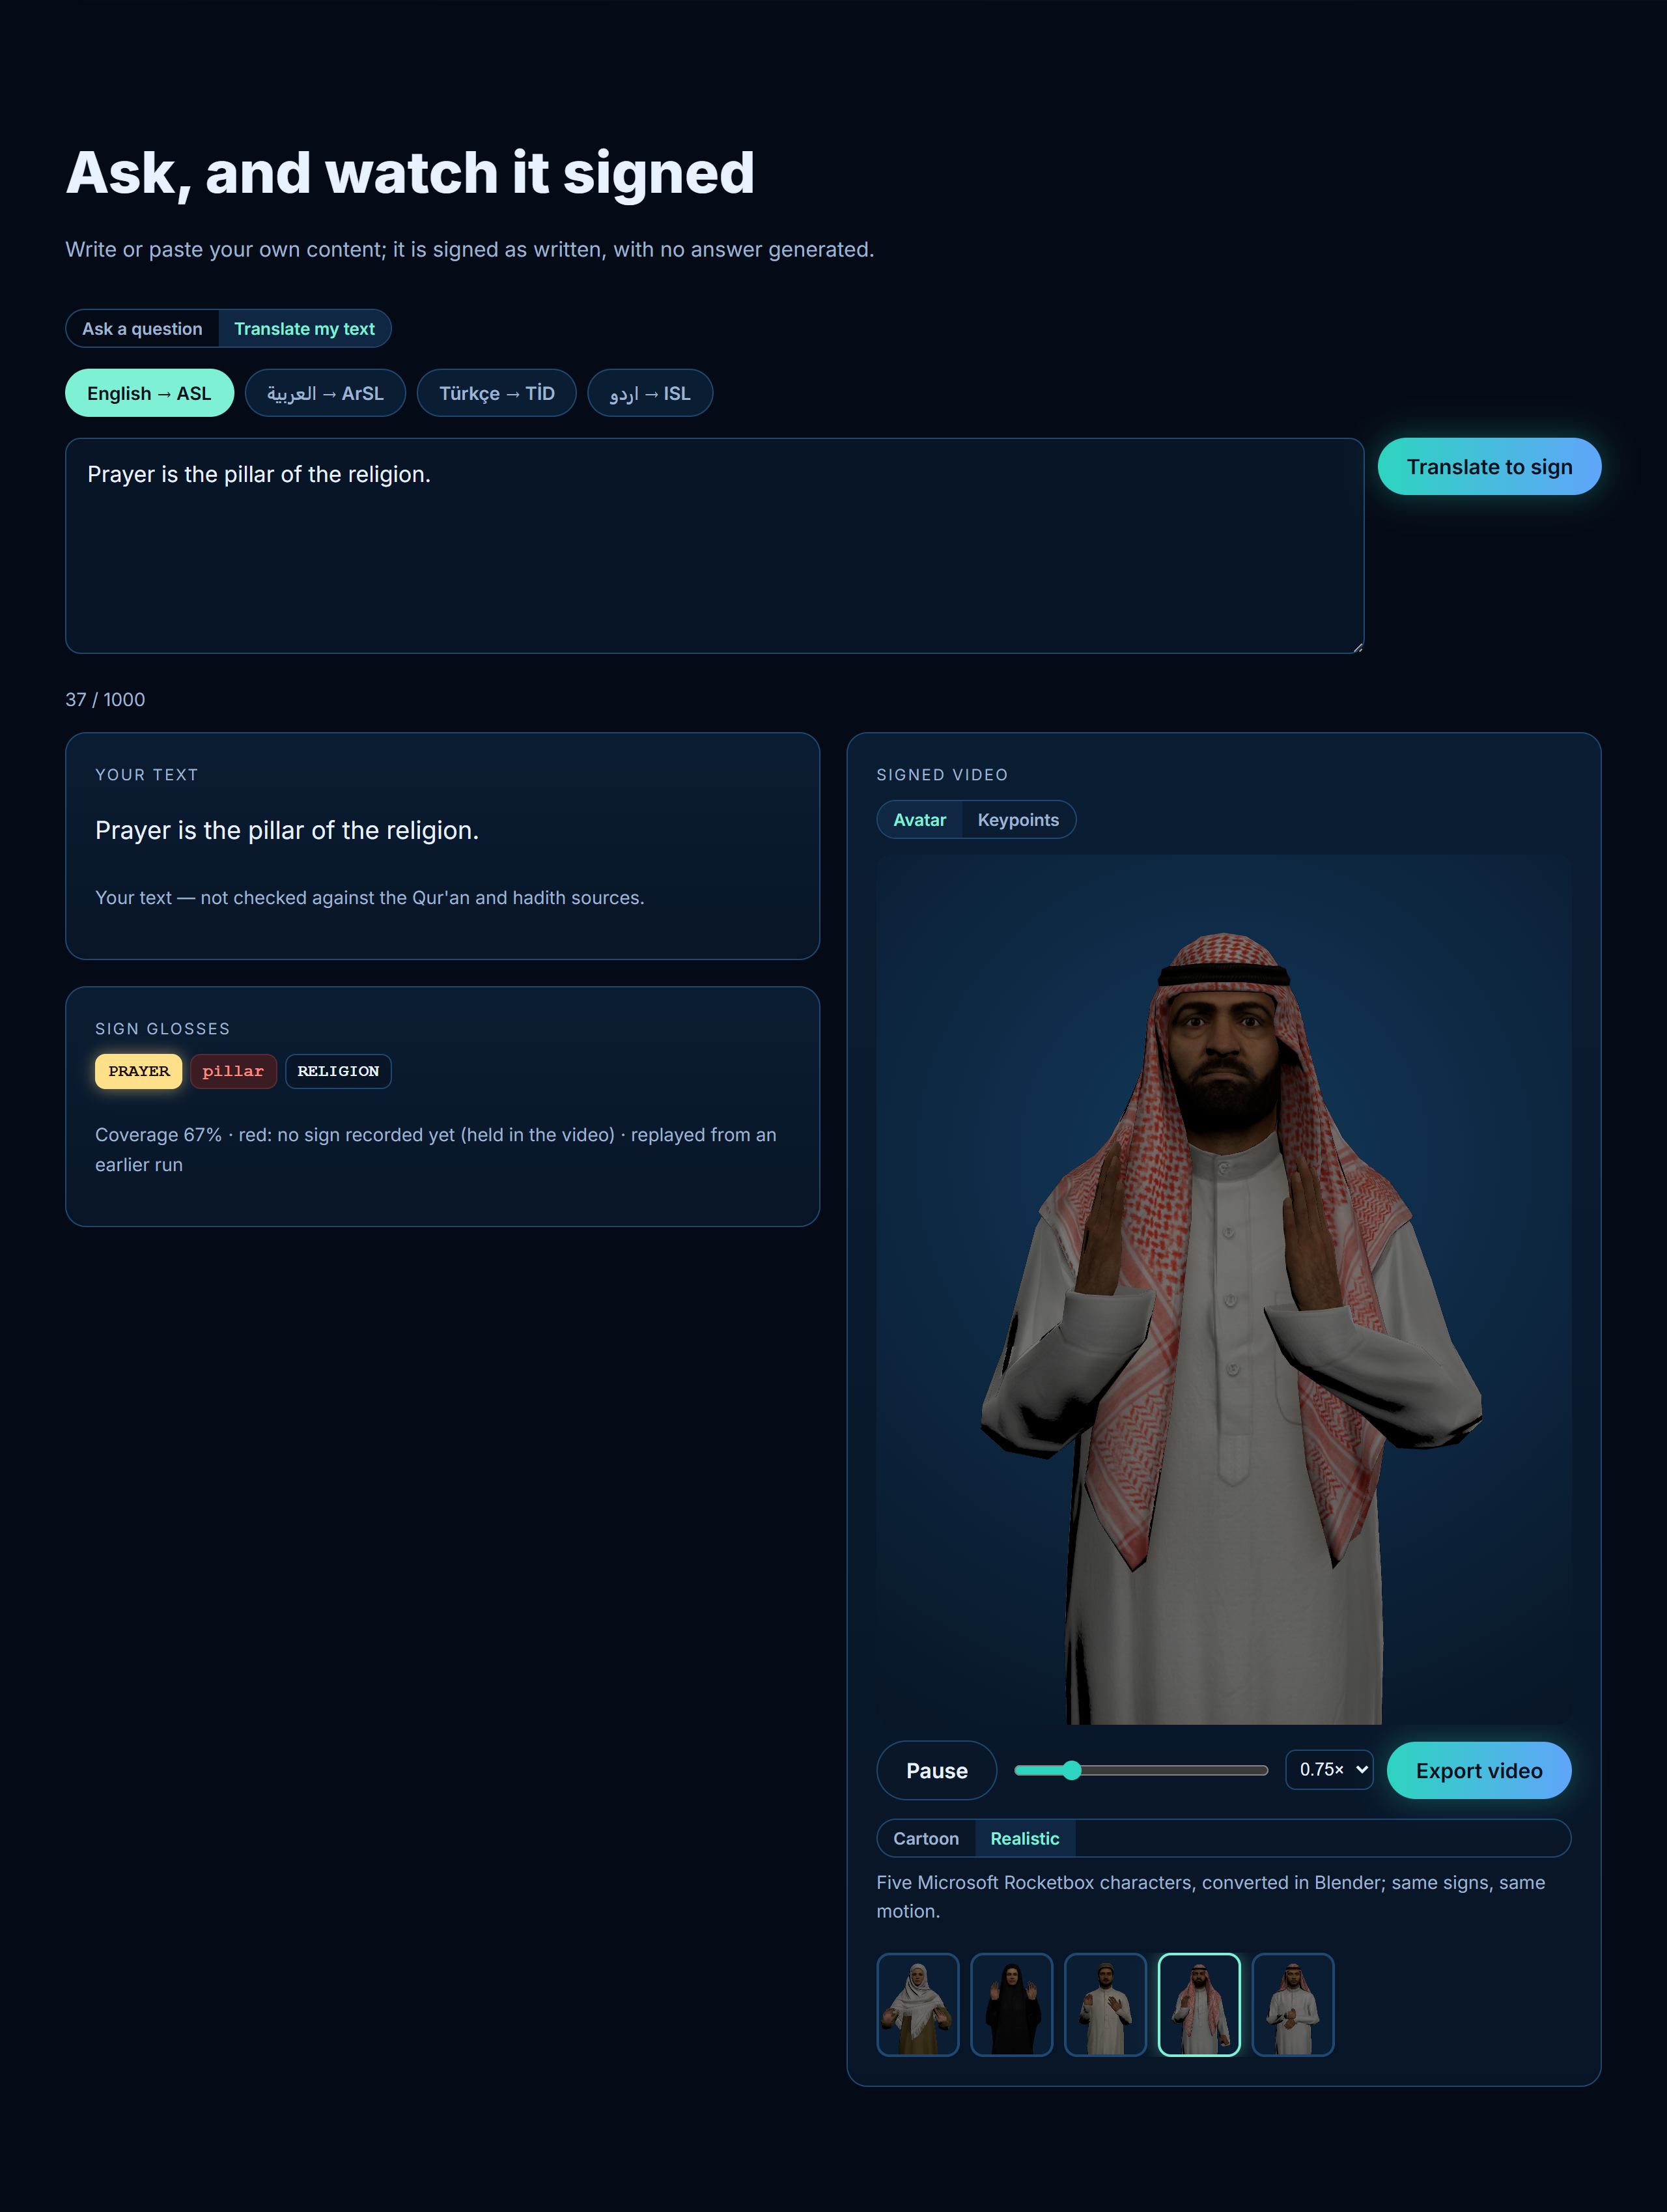
\includegraphics[width=\textwidth]{figures/ui_studio.png}
\caption{\textbf{Isharati Review Studio.}  The dual-panel annotation interface.
\textbf{Left panel:} Review queue of 6,112 seeded signs, filterable by two independent drop-down
menus --- \emph{Review Status} (All Signs, Needs Revision / Pending, Approved, Needs Modification,
Rejected) and \emph{Collection / Dataset} (12 collections listed in Table~\ref{tab:review_collections}).
Each queue entry shows the Arabic gloss, its colour-coded status badge, and the source dataset tag.
\textbf{Right panel:} Sign playback studio --- side-by-side 3D avatar rendering and skeletal keypoint
overlay, transport controls (play/pause, scrub bar, speed selector 0.5$\times$, 0.75$\times$,
1$\times$), and the three annotator decision buttons (Approved, Needs Modification, Rejected) with a
free-text notes field.  An integrated webcam recording module lets an expert re-record a corrected
physical gesture on the spot and upload it to the dataset repository.}
\label{fig:review_studio}
\end{figure}

\subsection{Dual-Axis Filtering}

The queue panel exposes two cascading filters:
\begin{enumerate}[leftmargin=*,itemsep=2pt]
  \item \textbf{Review Status filter} --- selects signs by their current verification state:
    \emph{All Signs} (6,112 total),
    \emph{Needs Revision / Pending},
    \emph{Approved},
    \emph{Needs Modification}, or
    \emph{Rejected}.
  \item \textbf{Collection / Dataset filter} --- restricts the queue to one of the 12 source
    collections (Table~\ref{tab:review_collections}).
\end{enumerate}
Applying both filters simultaneously (e.g., ``Pending signs from the Broadcast Sources collection'')
produces a targeted work-list that lets annotators focus on the highest-priority gaps without
wading through already-approved material.

\begin{table}[ht]
\centering\small
\caption{The 12 sign collections exposed in the Review Studio dataset filter, with their seeded
sign counts and extraction modality.  The \emph{Isharah Corpus Mined} row holds the 1,113
glosses mined from continuous Saudi Sign Language sentences; they were later found to be mis-segmented (Section~\ref{sec:lexicons})
and are excluded from the lexicon until re-mined.}
\label{tab:review_collections}
\begin{tabularx}{\textwidth}{L{4.6cm} r L{2.4cm} Y}
\toprule
Collection & Signs & Modality & Notes \\
\midrule
New Broadcast Sources & 2,409 & Continuous & 249 broadcast videos, 20 religious channels \\
Unified Arabic Dictionary & 1,283 & Isolated & Pan-Arab standardized dictionary \\
Kuwaiti Sign Dictionary & 975 & Isolated & Gulf and Kuwaiti dialect \\
KArSL Saudi Benchmark & 492 & Isolated & 3 native Deaf Saudi signers \\
Qur'an Curriculum (Al-Kharj) & 305 & Continuous & Word-by-word Qur'anic recitation \\
Tawasol Islamic Center & 196 & Continuous & Islamic pillars \& conversational signs \\
Scouts' Sign Dictionary & 139 & Isolated & Arab Scouting vocabulary \\
Levantine / Jordan Shorts & 110 & Continuous & Jordanian and Palestinian dialect \\
Children's Sign Dictionary & 87 & Isolated & Pediatric and educational signs \\
Arabic Dictionary Explained & 43 & Isolated & Morphological explanations \\
Saudi Dictionary Explained & 39 & Isolated & Saudi linguistic glosses \\
Isharah Corpus Mined & 34 & Continuous & RoPE-extracted continuous Saudi signs \\
\midrule
\textbf{Total} & \textbf{6,112} & & \\
\bottomrule
\end{tabularx}
\end{table}

\subsection{Isolated vs.\ Continuous Sign Inventory}

A critical distinction in the review process is the source modality of each sign recording, because
this directly affects the expected visual quality and review criteria applied by annotators:

\begin{itemize}[leftmargin=*,itemsep=2pt]
  \item \textbf{Isolated signs} (3,019 signs, 49.4\% of the seeded pool) originate from dedicated
    dictionary videos where a single word is performed without surrounding context.  Each recording
    is clean, includes the preparation and retraction strokes, and is labelled directly by the
    dictionary publisher.  Review focuses on handshape accuracy and cultural appropriateness.
  \item \textbf{Continuous segmented signs} (3,093 signs, 50.6\%) were algorithmically extracted
    from long-form signing streams (lessons, broadcasts, recitations) using the RoPE Transformer
    boundary model (Section~\ref{sec:rope_segmentation}).  Automatic segmentation of continuous
    signing is not reliable yet (best boundary F1 within $\pm4$ frames: 44.6\% on synthetic streams,
    Table~\ref{tab:segmentation_benchmark}), so these clips may contain partial strokes, truncated
    holds, or co-articulation bleed from adjacent glosses.  Review of this subset therefore also evaluates segmentation precision
    and temporal completeness.
\end{itemize}

Table~\ref{tab:isolated_vs_continuous} summarises the isolated vs.\ continuous breakdown per
source language and collection:

\begin{table}[ht]
\centering\small
\caption{Isolated vs.\ continuous sign breakdown across the full 6,112-sign review pool.
``Isolated'' denotes dictionary-style single-word recordings; ``Continuous'' denotes signs
extracted by the RoPE Transformer segmentation pipeline from broadcast, recitation, or lesson
streams.}
\label{tab:isolated_vs_continuous}
\begin{tabular}{l r r r}
\toprule
Source Group & Isolated & Continuous & Total \\
\midrule
Islamic Broadcast Sources (20 channels) & 0 & 2,409 & 2,409 \\
Unified Arabic Dictionary & 1,283 & 0 & 1,283 \\
Kuwaiti Sign Dictionary & 975 & 0 & 975 \\
KArSL Saudi Benchmark & 492 & 0 & 492 \\
Qur'an Curriculum (Al-Kharj) & 0 & 305 & 305 \\
Tawasol Islamic Center & 0 & 196 & 196 \\
Scouts' Sign Dictionary & 139 & 0 & 139 \\
Levantine / Jordan Shorts & 0 & 110 & 110 \\
Children's Sign Dictionary & 87 & 0 & 87 \\
Arabic Dictionary Explained & 43 & 0 & 43 \\
Saudi Dictionary Explained & 39 & 0 & 39 \\
Isharah Corpus Mined & 0 & 34 & 34 \\
\midrule
\textbf{Total} & \textbf{3,019} & \textbf{3,093} & \textbf{6,112} \\
\textbf{Share} & \textbf{49.4\%} & \textbf{50.6\%} & \textbf{100\%} \\
\bottomrule
\end{tabular}
\end{table}

\subsection{Playback and Decision Workflow}

Selecting any sign from the queue loads its $[T, 50, 3]$ pose tensor in real time.  The playback
panel renders the sign simultaneously as:
\begin{itemize}[leftmargin=*,itemsep=2pt]
  \item a \textbf{3D VRM avatar} (choice of Rocketbox Male/Female, hijab, shemagh, or thobe
    outfit), with kinematic retargeting applied to the 50 normalized joints;
  \item a \textbf{skeletal keypoint overlay} --- upper-body bones in teal, right-hand 21-joint
    chains in crimson, left-hand chains in sky blue --- using the normalized coordinate frame
    (neck at origin, shoulder-width unit scale).
\end{itemize}
Transport controls support variable playback speeds (0.5$\times$, 0.75$\times$, 1$\times$) and
frame-level scrubbing, enabling precise inspection of hold segments, transition smoothness, and
finger configurations.

Upon review the annotator issues one of three verdicts via the decision buttons:
\begin{enumerate}[leftmargin=*,itemsep=2pt]
  \item \textbf{Approved} --- the sign is accepted as a canonical lexicon entry and promoted to the
    production dataset (\url{https://huggingface.co/datasets/FatimahEmadEldin/isharati-review-signs}).
  \item \textbf{Needs Modification} --- the sign is linguistically valid but requires a technical
    correction (re-trimming, speed normalisation, or coordinate adjustment); the sign is queued
    for automated re-processing.
  \item \textbf{Rejected} --- the sign is incorrect (wrong handshape, wrong gloss label, or
    culturally inappropriate), and is removed from the production candidate pool.
\end{enumerate}
All decisions are written to the Neon PostgreSQL database with a timestamp and reviewer identifier,
providing a full audit trail.

\section{Normalization in the Review Process}
\label{sec:verification_normalization}

Signs displayed in the Review Studio are always shown in their \emph{normalized} form, not as raw
pixel coordinates.  The normalization pipeline (Section~\ref{sec:preproc}) applied before display
includes:
\begin{enumerate}[leftmargin=*,itemsep=2pt]
  \item \textbf{Shoulder-width normalization} --- all signers' bodies are rescaled so the neck
    is the spatial origin and the shoulder width equals one unit, eliminating camera distance and
    body proportion differences between dictionary and broadcast sources.
  \item \textbf{Coordinate system flip} --- the raw screen-space $+Y$-down axis is inverted to
    the anatomically natural $+Y$-up convention used by the 3D avatar skeleton.
  \item \textbf{Palm orientation and quaternion hemisphere continuity} --- an orthonormal palm
    frame $(\mathbf{u}_{\text{palm}}, \mathbf{v}_{\text{palm}}, \mathbf{n}_{\text{palm}})$ is
    constructed per frame; quaternion hemisphere flips that cause ``arm glitching'' during rapid
    wrist rotations are corrected by enforcing $\langle q_t, q_{t-1}\rangle \ge 0$, and angular
    jump spikes exceeding $2.0\,\text{rad}$ are replaced by SLERP interpolation.
  \item \textbf{Torso clearance clamping} --- a dynamic forward clearance boundary prevents hands
    from passing through the avatar's torso or robes ($Z_{\text{wrist}} \ge Z_{\text{shoulder}} +
    0.38 \times L_{\text{arm}}$), eliminating the clipping artifacts that would otherwise appear
    when a compressed skeletal window is rendered at normal avatar proportions.
\end{enumerate}
This means that annotators always see a clean, anatomically stable rendering regardless of the
original recording quality, and their judgment can focus on \emph{linguistic correctness} rather
than technical video artifacts.

\section{Expert Sign Language Annotation}
\label{sec:annotators}

\paragraph{Annotator.} The first expert review was carried out by \textbf{Ahmed Tahir}, a sign language expert
(B.Sc.\ in Computer Science, Arab Open University, Saudi branch) who has worked with the National Center for
Artificial Intelligence (NCAI) on a collaboration project on Saudi Sign Language. He reviewed signs in the Review Studio of the
deployed Space during a recorded online session on 4 October 2026 (Figures~\ref{fig:expert_meeting}, \ref{fig:expert_studio}
and~\ref{fig:expert_signing}), demonstrating the correct form of each sign on camera while judging the avatar's rendering.
Further annotators are being recruited, so that each sign can be judged by more than one expert and agreement measured.

\paragraph{What was reviewed.} The session covered the Qur'an-curriculum source (signs cut from the Al-Kharj Qur'an
curriculum videos, Section~\ref{sec:lexicons}), which supplies many of the Qur'anic content words. Each verdict is written to the
\code{sign\_reviews} table of the Neon PostgreSQL database with the sign identifier, gloss, source, decision and a
timestamp. Table~\ref{tab:expert_verdicts} lists all 22 human verdicts. Of the 3,209 seeded entries, the database also
holds about 2,900 rows marked approved or reviewed automatically when sources were imported (KArSL, new Arabic sources,
numbers and model signs); these are \emph{not} expert judgements and are excluded here. One test entry made while the
tool was being built is excluded too.

\begin{table}[ht]
\centering\small
\caption{Expert verdicts from the first review session (4 October 2026, Qur'an-curriculum signs; source: \code{sign\_reviews}).}
\label{tab:expert_verdicts}
\begin{tabularx}{\textwidth}{L{2.6cm} r Y}
\toprule
Verdict & Signs & Glosses \\
\midrule
Approved & 16 & \ar{الله، أشقى، تقوى، سوى، غشي، نهار، ضحى، مؤصدة، عقبة، غير، صراط، ليلة، صالحة، وجد، أعطى، ليل} \\
Needs modification & 1 & \ar{مسكين} \\
Rejected & 5 & \ar{ذكر، تلى، اسم، عابد، أرض} \\
\midrule
Total & 22 & approval rate 72.7\,\% (16/22); acceptable after correction 77.3\,\% (17/22) \\
\bottomrule
\end{tabularx}
\end{table}

\paragraph{What the verdicts changed.} The rejections were acted on straight away:
\begin{itemize}[leftmargin=*,itemsep=2pt]
  \item \ar{عابد} (worshipper) was rejected as a sign. On the expert's advice it is now \emph{fingerspelled}
    letter by letter (\ar{ع ا ب د}) from the KArSL letter signs, recorded as a reviewed decision
    (\code{reviewed\_fingerspelling}), and the same treatment was extended to 22 names of the Companions
    (Section~\ref{sec:ar_norm}).
  \item \ar{ذكر}: the rejected clip turned out to be shared between two senses of the word (\emph{remembrance} and
    \emph{male}); the SignBank rows that reused it for \ar{الرجل} were later rejected for the same reason
    (Section~\ref{sec:ar_norm}).
  \item The remaining rejected signs stay out of production until they are re-recorded or replaced from another source.
\end{itemize}

\begin{figure}[ht]
\centering
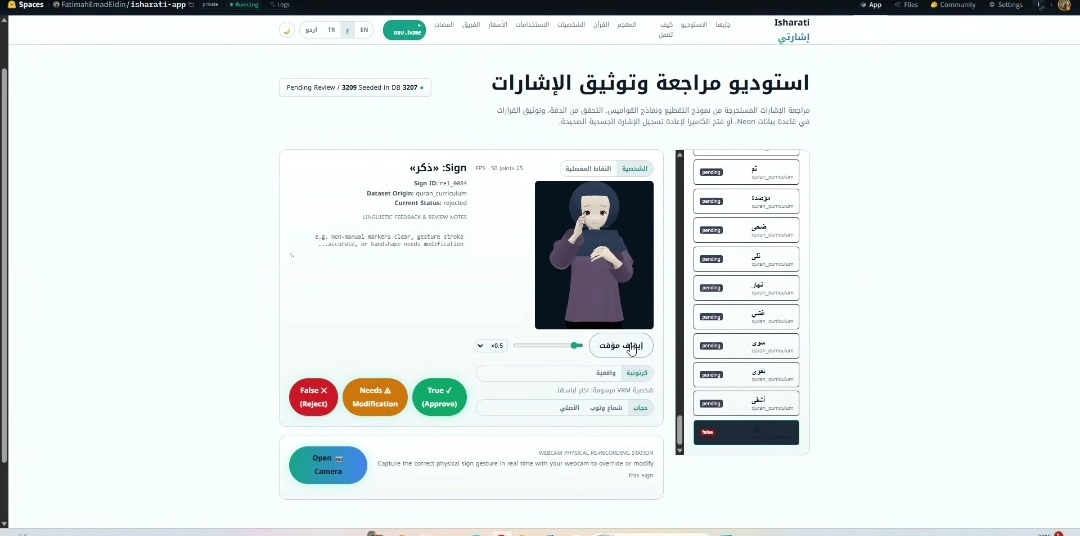
\includegraphics[width=0.49\textwidth]{figures/expert_review/studio_dhikr_rejected.jpg}\hfill
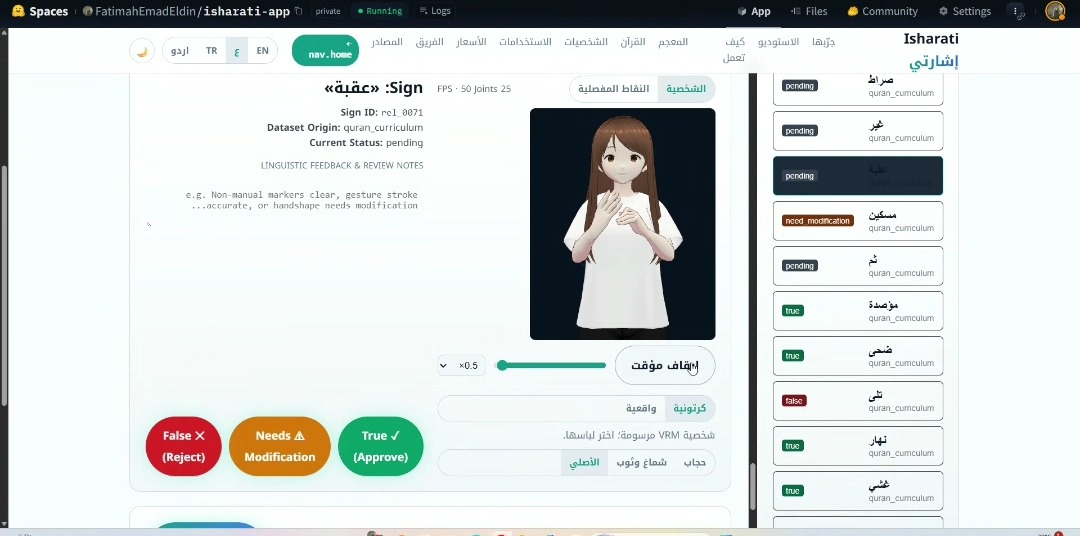
\includegraphics[width=0.49\textwidth]{figures/expert_review/studio_aqaba.jpg}
\caption{The Review Studio during the expert session. Left: \ar{ذكر}, rejected. Right: \ar{عقبة} played on the
cartoon avatar at 0.5$\times$, with the verdict buttons (False / Needs modification / True) and the queue of
Qur'an-curriculum signs with their statuses.}
\label{fig:expert_studio}
\end{figure}

\begin{figure}[ht]
\centering
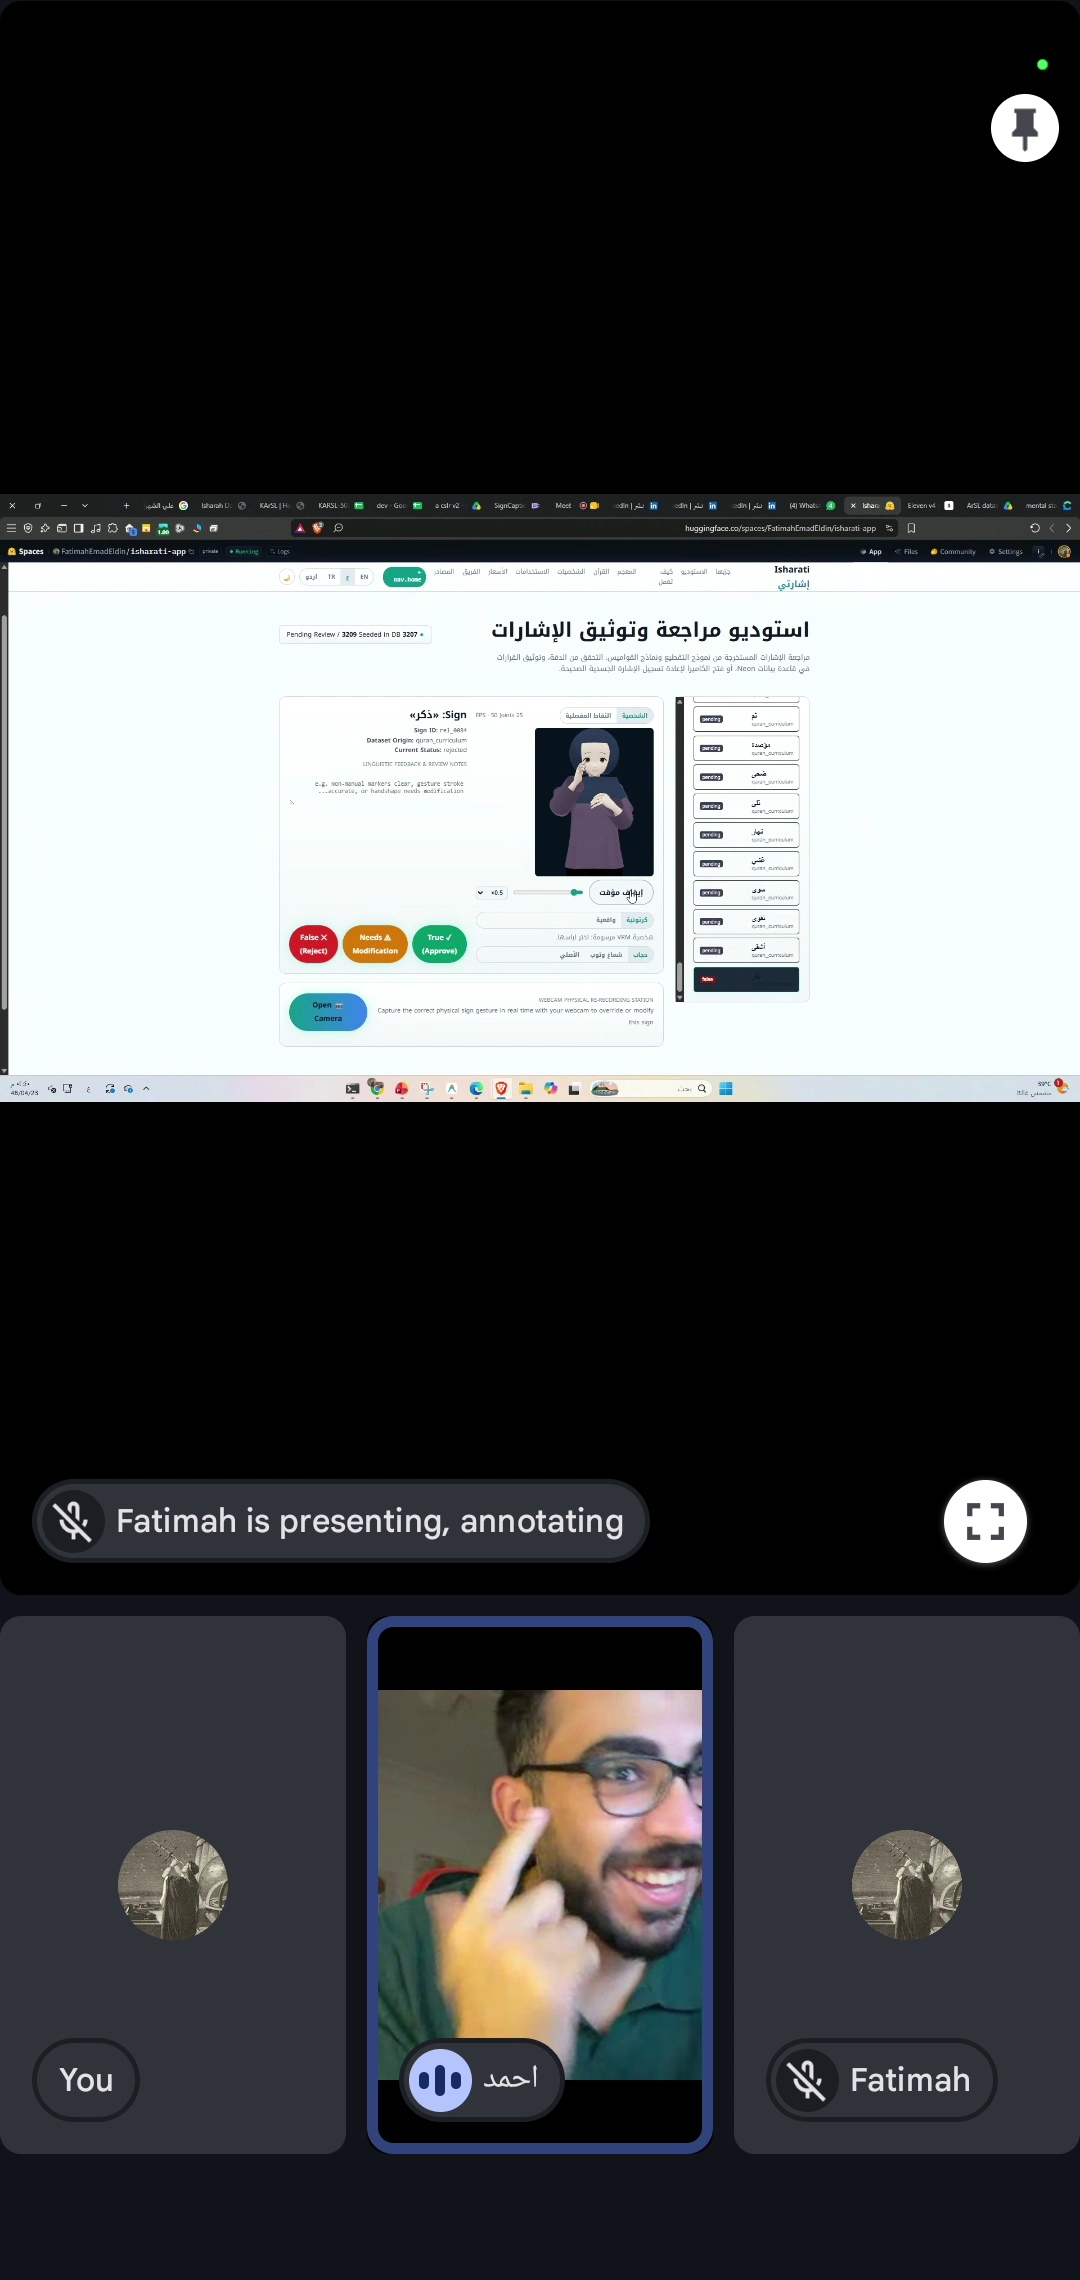
\includegraphics[width=0.32\textwidth]{figures/expert_review/meeting_full_1.jpg}\hfill
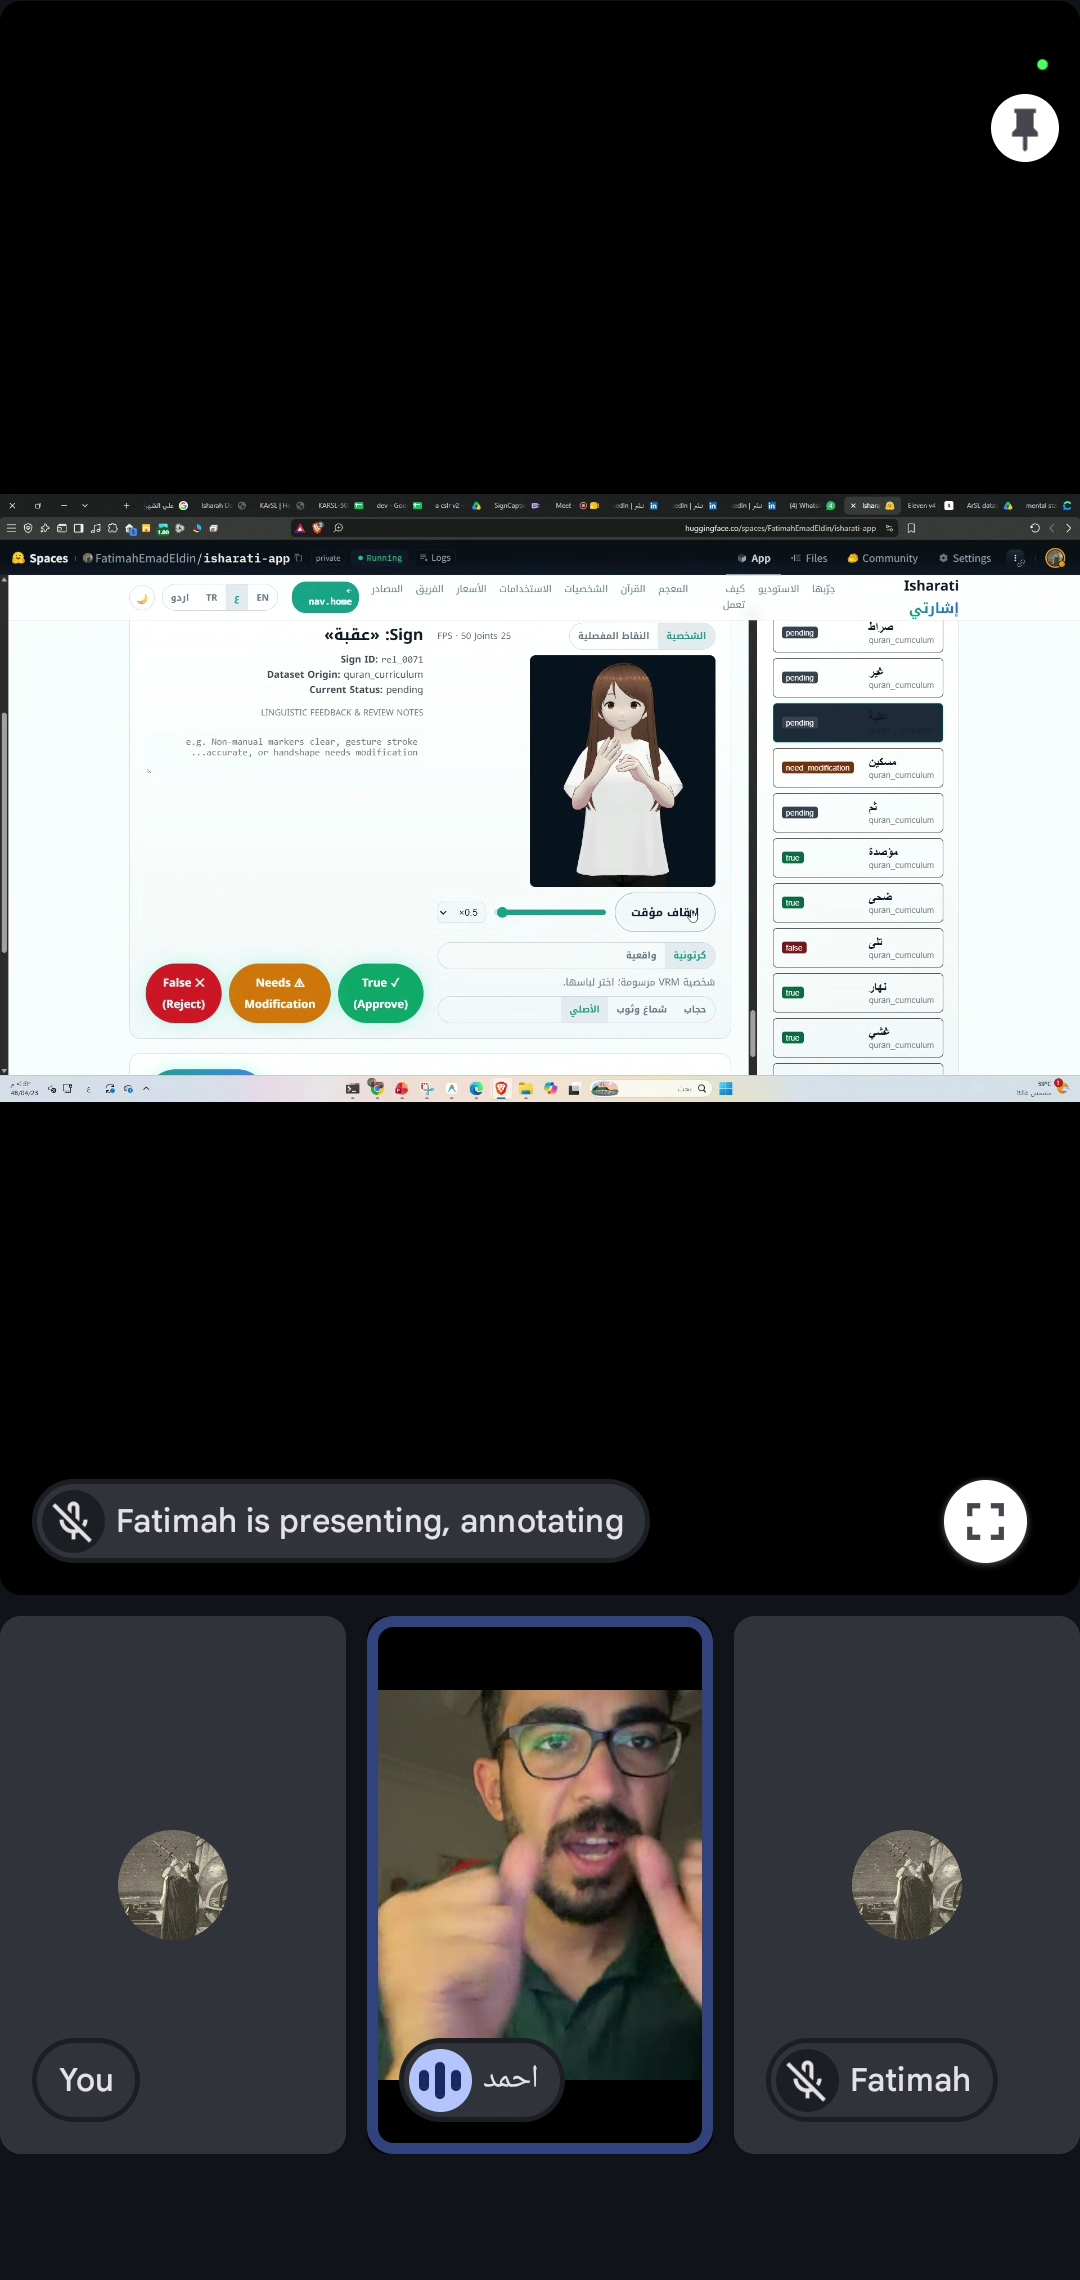
\includegraphics[width=0.32\textwidth]{figures/expert_review/meeting_full_2.jpg}\hfill
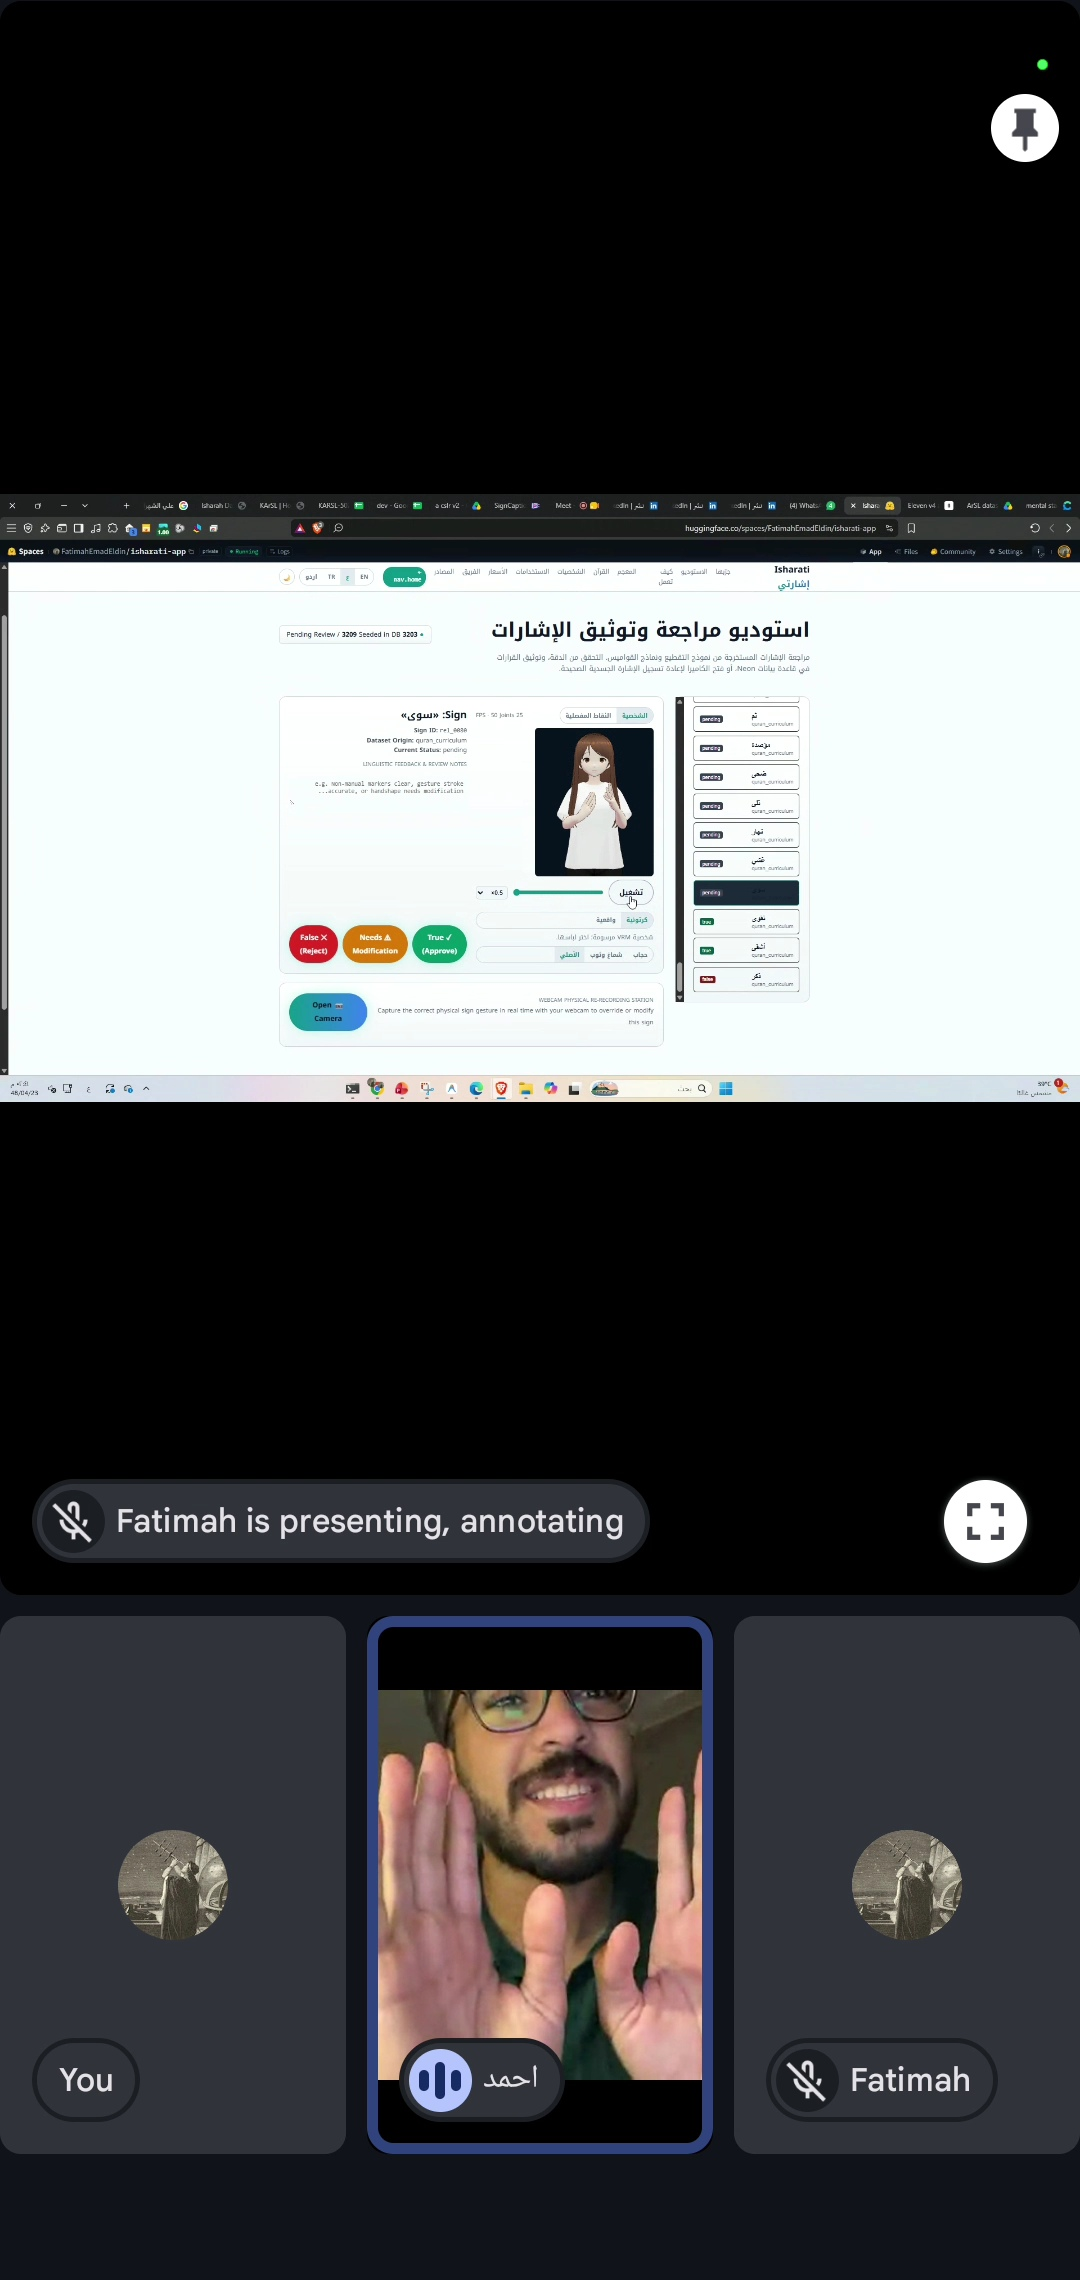
\includegraphics[width=0.32\textwidth]{figures/expert_review/meeting_full_3.jpg}
\caption{The online review session of 4 October 2026, uncropped: the Review Studio shared on screen while the expert, Ahmed
Tahir, demonstrates each sign on camera.}
\label{fig:expert_meeting}
\end{figure}

\begin{figure}[ht]
\centering

\includegraphics[width=0.8\textwidth]{figures/expert_review/expert_signing_grid.jpg}
\caption{The expert demonstrating signs on camera during the review session, used to judge and correct the avatar's
handshapes.}
\label{fig:expert_signing}
\end{figure}

\paragraph{Limits.} This is one expert and 22 signs: enough to catch systematic problems (the shared-clip sense error,
the need to fingerspell a word), not to estimate the precision of the whole lexicon. The next step is a stratified
sample across sources, judged by at least two experts, with inter-annotator agreement reported.

\section{Summary}

The Review Studio turns the automatically built lexicon into one that experts can check sign by sign, with every
decision stored and traceable. The first expert session approved 16 of 22 signs, and its rejections led directly to
fixes in the lexicon (fingerspelling and the removal of a shared clip with two meanings). The review is ongoing; verified signs will be released
in the \code{isharati-review-signs} Hugging Face dataset with the annotation log (reviewer, timestamp, decision, notes).

\chapter{Discussion, limitations and future work}
\label{sec:discussion}

\section{System achievements and technical guarantees}
Isharati addresses the long-standing challenge of digital sign language access for sacred Islamic scripture by enforcing strict architectural guarantees across its pipelines:
\begin{enumerate}[leftmargin=*,itemsep=2pt]
  \item \textbf{Grounded theological integrity:} Factuality is enforced deterministically after generation rather than relying on LLM self-consistency. Any sentence not fully supported by retrieved Qur'an or hadith passages is excised, and legal ruling inquiries (*fatawa*) are immediately intercepted and referred to human scholars.
  \item \textbf{Transparent lexical tracking:} Rather than synthesizing approximate or fabricated handshapes, signing is synthesized from verified, canonical motion captures. Words lacking a verified sign are reported transparently in the user interface and held in rest rather than obscured by fingerspelling.
  \item \textbf{Scalable weakly supervised vocabulary expansion:} By deploying a 5-layer dilated temporal convolutional network with multiple-instance learning over 21 million frames of continuous YouTube-ASL, the platform successfully mined 186 missing scriptural terms, driving content-word coverage to \textbf{80.96\%} and demonstrating that skeletal kinematics alone carry sufficient signal for weakly supervised sign discovery.
  \item \textbf{Culturally grounded photorealistic 3D avatars:} The automated conversion of Microsoft Rocketbox humanoid meshes into VRM 1.0, paired with WebGL kinematic retargeting and procedural modesty attire (hijab and shemagh), brings high-fidelity, culturally respectful signing into standard mobile and desktop web browsers without video-streaming latency.
\end{enumerate}

\section{Current limitations and considerations}
While Isharati represents a major functional leap forward, several technical and linguistic considerations remain active areas of refinement:
\begin{enumerate}[leftmargin=*,itemsep=2pt]
  \item \textbf{Community-in-the-loop review:} Although automated multi-source consensus, kinematic validity filters, and spotter confidence thresholds classify the vast majority of mined signs as high-confidence candidates (153 approved, 30 requiring light review), community review by Deaf native signers and scholars remains essential prior to official curricular adoption.
  \item \textbf{Concatenation and grammatical prosody:} The current poser joins discrete sign recordings using cubic Hermite smoothstep interpolation and proportional bone rescaling. While transitions are smooth and eliminate abrupt visual pops, natural sign languages employ complex co-articulation, use 3D signing space for pronominal and spatial referencing, and convey critical grammatical mood through facial non-manual markers.
  \item \textbf{Evolution of back-translation metrics:} Early baselines relied on cross-signer 1-nearest-neighbour dynamic time warping, which suffered from inter-signer morphological variance. The platform has largely moved beyond this towards neural verification: our weakly supervised MIL spotter achieves a $60\times$ improvement over chance on continuous video data, and neural continuous sign language recognition (CSLR) models reach $\sim$3\% WER on benchmark data. Fully scaling continuous neural back-translation to evaluate complete concatenated sentence outputs across all four target languages remains an ongoing engineering effort.
  \item \textbf{Dialectal diversity:} Arabic Sign Language encompasses several regional dialects (Saudi, Levantine, Egyptian, and Gulf). Isharati explicitly tags each sign's provenance in its metadata schema, enabling regional filtering, but unified dialect standardization requires continued engagement with local Deaf associations.
  \item \textbf{Non-manual facial articulation:} At present, Isharati leverages 50 skeletal keypoints (8 upper body and $2 \times 21$ hand landmarks). Although facial landmarks are extracted during preprocessing (468 landmarks), active avatar rendering is focused on manual phonology; integrating real-time facial blendshapes (eyebrows, mouthings, and eye gaze) will further elevate linguistic richness.
\end{enumerate}

\section{Future work}
Immediate next steps build directly upon the platform's modular foundation:
\begin{itemize}[leftmargin=*,itemsep=2pt]
  \item \textbf{End-to-end continuous translation models:} Fine-tuning continuous sequence-to-sequence translation architectures (such as T5-for-SLT) to map natural language directly into fluent, grammatically reordered continuous sign sequences, capturing co-articulation and sign-space topography.
  \item \textbf{Facial blendshapes and non-manual markers:} The signed hadith samples now carry the signer's 52 face blendshape scores, which drive the avatar's ARKit shapes directly (Chapter~\ref{sec:scripture}); the same pass still has to be run over the Qur'an datasets and the lexicon, and the grammatical markers (questioning eyebrow raises, head tilts, mouth morphemes) have yet to be evaluated as such.
  \item \textbf{Completing the signed hadith corpus:} Processing the four silent lesson series (65.7 hours, one sample per hadith rather than per video), aligning signs inside each hadith, and having Deaf reviewers check the labels that the on-screen and translation routes produce.
  \item \textbf{Broadened neural back-translation:} Expanding fine-tuned continuous neural back-translation models across Turkish Sign Language (T\.{I}D) and Indo-Pakistani Sign Language (ISL) to provide unified, automated quality certificates for all four language pipelines.
  \item \textbf{Participatory community evaluation:} Conducting structured empirical comprehension and naturalness evaluations with Deaf students, educators, and Islamic scholars across Saudi Arabia and the wider Islamic world.
\end{itemize}

\chapter{Commercialization Strategy, Business Model, and Strategic Market Analysis}
\label{sec:business}

\section{Market Opportunity and Strategic Rationale}
\label{sec:biz_opportunity}
Digital accessibility for Deaf communities has historically been an acute blind spot across the Muslim world. According to the World Health Organization (WHO), over 430 million individuals globally experience disabling hearing loss, with approximately 70 million profoundly Deaf people communicating natively through more than 300 distinct visual-gestural sign languages. Within the global Muslim population exceeding 1.9 billion adherents, an estimated 15 to 20 million Deaf Muslims face structural linguistic isolation when attempting to engage with foundational scripture (the Qur'an and Hadith), weekly congregational prayers, and religious education.

\paragraph{The Religious Accessibility Divide.}
While spoken and printed translations, high-fidelity audio recitations, and mobile applications have democratized sacred Islamic content for hearing populations worldwide, the Deaf Ummah remains largely disenfranchised. Sign languages are spatial, non-concatenative natural languages possessing independent syntax and grammar that diverge radically from linear spoken or written tongues; for the vast majority of Deaf individuals, written Classical or Modern Standard Arabic functions as an unfamiliar second or foreign language. Traditional efforts to bridge this divide rely on scarce human interpreters whose availability is constrained by prohibitive market rates (\$50--\$120 per hour) and a systemic absence of accredited theological training. Consequently, Friday congregational sermons (\textit{khutbahs}), daily mosque lectures, madrasah curricula, and international Islamic media remain overwhelmingly inaccessible.

\paragraph{Market Sizing: TAM, SAM, and SOM.}
To quantify the strategic commercial opportunity, we apply a top-down and bottom-up market sizing framework across the Islamic digital economy and assistive technology landscape:
\begin{itemize}[leftmargin=*,itemsep=3pt]
  \item \textbf{Total Addressable Market (TAM) --- \$1.85 Billion:} Encompasses the global religious assistive technology, faith-based educational publishing, and digital Islamic economy sectors spanning 1.9 billion Muslims across 57 OIC member states and global diaspora communities. This includes government accessibility compliance allocations, religious endowment (\textit{awqaf}) media digitization funds, and commercial Islamic media production.
  \item \textbf{Serviceable Available Market (SAM) --- \$340 Million:} Represents the addressable market within the Middle East, North Africa (MENA), and high-adoption Muslim populations in Europe, North America, and Southeast Asia (Turkey, Malaysia, Indonesia, Pakistan). This focuses on registered mosques, Islamic schools, ministries of religious affairs, and digital Islamic software publishers with active IT or accessibility budgets.
  \item \textbf{Serviceable Obtainable Market (SOM) --- \$42 Million:} The target market capture within the first 36 months of commercial deployment, focusing on institutional Friday sermon subscriptions across Saudi Arabia, the GCC, and premier urban mosques globally, alongside developer SDK integrations into top-tier mobile applications (e.g., Quran.com, Muslim Pro, Tarteel) and philanthropic endowment grants.
\end{itemize}

\paragraph{Macro Regulatory and Institutional Drivers.}
The commercial launch of Isharati is strategically aligned with powerful institutional catalysts:
\begin{itemize}[leftmargin=*,itemsep=2pt]
  \item \textbf{Saudi Vision 2030 and DGA Compliance:} The Saudi Digital Government Authority (DGA) and Ministry of Human Resources mandate strict digital accessibility benchmarks across all public, civic, and religious digital platforms.
  \item \textbf{Global UN CRPD Mandates:} The United Nations Convention on the Rights of Persons with Disabilities explicitly obligates member nations to recognize and provide sign language access across education, public service, and civic life.
  \item \textbf{Institutional Awqaf and Da'wah Budgets:} Millions of dollars are disbursed annually by ministries of Islamic affairs and private endowments for international translation. Transitioning a fractional share of these existing allocations into automated, verified sign language pipelines yields immediate, measurable social impact.
\end{itemize}

\section{Competitive Landscape and Strategic Differentiation}
\label{sec:biz_competition}
The assistive sign language market is nascent and fragmented into localized startups and generic academic prototypes. Table~\ref{tab:competitor_matrix} benchmarks Isharati against prominent commercial platforms, including recent AI sign generation tools (such as GoSign AI and SignCaption AI), legacy commercial providers, and generalist laboratory prototypes.

\begin{table}[ht]
\centering\small
\caption{Strategic benchmark of Isharati against contemporary commercial and research sign language platforms.}
\label{tab:competitor_matrix}
\begin{tabularx}{\textwidth}{L{2.6cm} L{2.2cm} L{2.6cm} L{2.2cm} Y}
\toprule
Platform & Primary Focus & Linguistic Engine & Rendering Tech & Key Deficiencies \& Commercial Limitations \\
\midrule
GoSign AI & Web accessibility \& marketing & Generic MT + gloss lookup & WebGL humanoid avatar & Western Sign Languages (ASL/BSL); no Arabic morphological awareness; zero religious coverage. \\
SignCaption AI & Video captioning \& social clips & Whisper ASR + heuristic glossing & Server-rendered video overlay & High video cloud rendering cost (\$0.80--\$2.00/min); lacks 3D interactive controls; no scripture verification. \\
Kara Technologies & Children's media \& education & Rule-based NLP glossing & Cloud GPU video streaming & High infrastructure overhead (\$2.00/min); closed proprietary ecosystem; no Semitic NLP or Islamic grounding. \\
SignAll & Sign recognition \& kiosks & Multi-camera computer vision & Sensor-driven UI & Hardware-intensive; focuses on sign-to-text recognition rather than expressive generation; non-scalable. \\
\midrule
\textbf{Isharati (Ours)} & \textbf{Sacred Islamic scripture \& education} & \textbf{Hybrid RAG + CAMeL Semitic morphology} & \textbf{Zero-cost client WebGL (VRM 1.0)} & \textbf{Theologically guarded; halal/modest procedural avatars; full 114 Surah Qur'an coverage; edge-deployable.} \\
\bottomrule
\end{tabularx}
\end{table}

\paragraph{Strategic Defensibility and Moats.}
Competitors face prohibitive barriers to entry when attempting to replicate Isharati due to four proprietary defensibility moats:
\begin{enumerate}[leftmargin=*,itemsep=2pt]
  \item \textbf{Theological Grounding and Hallucination Immunity:} Mainstream generative models produce unverified text approximations that risk introducing grave theological errors into sacred rulings. Isharati enforces strict deterministic hallucination guards: ungrounded assertions are stripped by our post-generation verifier, while legal ruling queries (\textit{fatawa}) are systematically intercepted and directed to human scholarly bodies.
  \item \textbf{Deep Semitic Morphological Disambiguation:} General-purpose tokenizers fail on Classical Arabic's clitic-rich morphology. Isharati integrates CAMeL Tools morphological analyzers to decompose prefixes, enclitics, and root lemmas before lexicon lookup, ensuring grammatically flawless sign synthesis.
  \item \textbf{Weakly-Supervised MIL Lexicon Mining:} Commercial sign dictionaries lack religious terminology. Our Multiple Instance Learning (MIL) spotter continuously extracts and aligns sign keypoints from real-world Arabic sign broadcasts, expanding vocabulary without manual studio capture bottlenecks.
  \item \textbf{Culturally Authentic, Zero-Cost Client Kinematics:} Unlike Western avatars, Isharati offers respectful 3D digital humans equipped with procedural modesty attire (hijab and shemagh), driven directly in client browsers without server-side video rendering expenses.
\end{enumerate}

\section{Monetization Models and Revenue Channels}
\label{sec:biz_monetization}
Isharati deploys a multi-tiered, diversified business model addressing individual creators, institutional establishments, mobile application developers, and governmental agencies (Figure~\ref{fig:biz_model}).

\begin{figure}[ht]
\centering
\resizebox{\textwidth}{!}{%
\begin{tikzpicture}[
  node distance=6mm and 8mm,
  core/.style={draw=navy, fill=soft, rounded corners=3pt, font=\small\bfseries, align=center, text width=38mm, minimum height=14mm},
  chan/.style={draw=tealx!80!black, fill=tealx!10, rounded corners=2pt, font=\footnotesize, align=center, text width=32mm, minimum height=12mm},
  cust/.style={draw=amberx!90!black, fill=amberx!12, rounded corners=2pt, font=\footnotesize, align=center, text width=32mm, minimum height=12mm},
  arr/.style={-{Stealth[length=2mm]}, thick, navy}]
  
  \node[core] (core) {Isharati Core Engine\\(RAG + CAMeL Morphology\\+ Kinematic WebGL Engine)};
  
  \node[chan, above left=8mm and 4mm of core] (saas) {\textbf{1. B2B / B2G SaaS}\\Studio Web App, Live ASR,\\Khutbah Sign Broadcast};
  \node[chan, above right=8mm and 4mm of core] (sdk) {\textbf{2. Developer Cloud SDK}\\Headless REST APIs\\+ WebGL Avatar SDK};
  \node[chan, below left=8mm and 4mm of core] (daas) {\textbf{3. Data-as-a-Service}\\Domain Lexicon Mining\\+ Verified Pose Corpora};
  \node[chan, below right=8mm and 4mm of core] (edge) {\textbf{4. Edge Appliance / B2G}\\On-Premise Jetson Boxes\\\& Sovereign Digital Twins};

  \node[cust, left=6mm of saas] (mosques) {Mosques, Preachers\\\& Awqaf Ministries};
  \node[cust, right=6mm of sdk] (apps) {Islamic Mobile Apps\\(Quran \& Prayer Apps)};
  \node[cust, left=6mm of daas] (research) {Academic \& Assistive\\Tech Organizations};
  \node[cust, right=6mm of edge] (gov) {Rural / Remote Mosques\\\& Education Authorities};

  \draw[arr] (core) -- (saas); \draw[arr] (core) -- (sdk); \draw[arr] (core) -- (daas); \draw[arr] (core) -- (edge);
  \draw[arr] (saas) -- (mosques); \draw[arr] (sdk) -- (apps); \draw[arr] (daas) -- (research); \draw[arr] (edge) -- (gov);
\end{tikzpicture}}
\caption{Isharati commercialization architecture: four core revenue streams serving institutional, educational, and developer stakeholders.}
\label{fig:biz_model}
\end{figure}

\subsection{1. Software-as-a-Service (SaaS) Subscriptions}
The core SaaS platform powers accessible content creation across educational and religious institutions:
\begin{itemize}[leftmargin=*,itemsep=2pt]
  \item \textbf{Mosque Khutbah Live Translation Module:} Provides automated speech-to-sign interpretation for Friday sermons. The imam's spoken audio is captured live via microphone or uploaded video, transcribed through Whisper-large-v3, normalized morphologically, and rendered on auxiliary mosque display monitors or live-streamed to Deaf attendees' smartphones.
  \item \textbf{Educator and Da'wah Studio:} Independent preachers, Islamic schools, and da'wah production houses subscribe to generate high-definition sign language reels, social clips, and educational modules in Arabic, Turkish, and Urdu sign dialects.
\end{itemize}

\subsection{2. Developer Cloud SDK and API-as-a-Service}
Developers of leading consumer Islamic platforms (reaching over 150 million aggregate active users across Quran.com, Muslim Pro, Tarteel, and Athkar) can embed sign language avatars natively into their applications:
\begin{itemize}[leftmargin=*,itemsep=2pt]
  \item \textbf{Headless REST Endpoints:} \code{POST /api/ask}, \code{POST /api/sign}, \code{POST /api/transcribe}, and \code{GET /api/quran/pose} provide word-level timings, morpho-syntactic gloss tags, and compressed $[T, 50, 3]$ kinematic arrays.
  \item \textbf{Embeddable WebGL SDK (\texttt{isharati-avatar.js}):} A lightweight, zero-dependency client widget executing in two lines of HTML, rendering 3D avatars directly in browser canvases at 60 FPS without server graphics rendering.
  \item \textbf{Metered Cloud Billing:} Charged at \$0.03 per minute of generated sign kinematics or \$0.005 per verified RAG query.
\end{itemize}

\subsection{3. Data-as-a-Service (DaaS) and Commissioned Mining}
For specialized theological and jurisdictional domains, Isharati licenses verified sign corpora and executes custom vocabulary mining:
\begin{itemize}[leftmargin=*,itemsep=2pt]
  \item \textbf{Commissioned Domain Lexicon Expansion:} Government ministries, Hajj/Umrah agencies, and Islamic banking institutions commission the extraction and validation of specialized glosses (e.g., Islamic finance contracts, pilgrimage rituals, Sharia court terms) priced from \$5,000 to \$150,000 per domain package.
  \item \textbf{Corpus Research Licensing:} Verified, time-aligned 3D skeletal keypoint datasets and gloss annotations are licensed to academic and corporate AI research laboratories.
\end{itemize}

\subsection{4. Edge Appliance for Rural and Remote Mosques}
To support rural and low-bandwidth sanctuaries that lack reliable high-speed fiber internet, Isharati packages an edge hardware appliance (powered by Nvidia Jetson Orin Nano or Raspberry Pi 5). The appliance runs quantized local ASR, cached offline Semitic lexicons, and zero-latency WebGL rendering over HDMI outputs directly to mosque projection displays, operating entirely air-gapped without recurring cloud bandwidth dependencies.

\section{Commercial Tiers and Packaging}
\label{sec:biz_tiers}
To maintain universal humanitarian access for individual Deaf Muslims while monetizing institutional and enterprise clients, Isharati deploys four clear commercial tiers (Table~\ref{tab:pricing_tiers}).

\begin{table}[ht]
\centering\small
\caption{Isharati subscription tiers, feature entitlements, and pricing matrix.}
\label{tab:pricing_tiers}
\begin{tabularx}{\textwidth}{L{2.2cm} L{2.2cm} L{3.0cm} Y}
\toprule
Tier & Pricing & Target Customer & Features and Capabilities \\
\midrule
\textbf{Community Free} & \$0 / forever & Deaf individuals, students, families & 15 minutes daily sign generation; full 114 Surah Qur'an coverage map; standard anime avatar; WebGL real-time browser rendering; community support. \\
\midrule
\textbf{Educator \& Creator} & \$29 / mo (\$24/mo annual) & Teachers, madrasahs, da'wah creators & 120 minutes monthly studio sign generation; all 6 photorealistic modesty avatars (Rocketbox + cartoon); procedural hijab/shemagh presets; 1080p MP4 export; CAMeL morphology analyzer studio; watermark removal. \\
\midrule
\textbf{Mosques \& Juma'a} & \$199 / mo (\$169/mo annual) & Neighborhood mosques, Islamic centers & Real-time Friday Khutbah live audio/video ASR transcription pipeline; multi-screen projector display integration; priority processing queue; offline fallback cache; institutional SLA. \\
\midrule
\textbf{Enterprise B2B / B2G} & \$25K--\$180K / yr (custom SLA) & Awqaf ministries, large apps, universities & Full Developer Cloud SDK \& REST APIs; custom 3D avatar digital twins; commissioned domain lexicon mining; dedicated on-premise container or Jetson edge appliance; 99.9\% uptime SLA. \\
\bottomrule
\end{tabularx}
\end{table}

\section{Cost Architecture and Unit Economics}
\label{sec:biz_economics}
A fundamental technical and economic breakthrough of Isharati is its client-edge architecture, which eliminates the unsustainable GPU rendering costs that have caused previous sign language startups to fail.

\paragraph{Unit Cost Mathematical Formulation.}
The direct Cost of Goods Sold ($\text{COGS}$) per user query is defined as:
\begin{equation}
\label{eq:cogs_formulation}
\text{COGS}_{\text{Query}} = C_{\text{LLM}} + C_{\text{emb}} + C_{\text{morph}} + C_{\text{transport}} + C_{\text{render}}
\end{equation}
Evaluating each component under production cloud rates:
\begin{itemize}[leftmargin=*,itemsep=2pt]
  \item \textbf{Language Model Inference ($C_{\text{LLM}}$):} Using open-weights models (Qwen 2.5 72B / Nemotron-3) via OpenRouter, a typical RAG prompt consumes $\approx$800 prompt tokens and generates $\approx$150 response tokens with verified citations. At \$0.60 per million tokens: $C_{\text{LLM}} \approx \$0.00057$.
  \item \textbf{Vector Embedding \& Retrieval ($C_{\text{emb}}$):} Multilingual E5-large query vectorization costs $\$0.00008$, with vector cosine search executed in-memory on the server.
  \item \textbf{Morphological Analysis ($C_{\text{morph}}$):} Fast vectorized CAMeL Tools lemmatization and gloss mapping execute on CPU in under 45\,ms: $C_{\text{morph}} \approx \$0.00020$.
  \item \textbf{Network Transport ($C_{\text{transport}}$):} Delivering structured JSON keypoint tensors ($<$180\,KB compressed) costs $\$0.00165$ in egress bandwidth.
  \item \textbf{Rendering Overhead ($C_{\text{render}}$):} Because 3D retargeting and skeletal deformation occur locally in the client's WebGL browser engine, the server-side rendering cost is \textbf{strictly \$0.00000}.
\end{itemize}
Summing these components yields a total direct marginal cost of:
\begin{equation}
\text{COGS}_{\text{Query}} = \$0.00057 + \$0.00008 + \$0.00020 + \$0.00165 + \$0.00000 \approx \mathbf{\$0.0025}
\end{equation}

\paragraph{Economic Comparison with Cloud Video Rendering.}
Legacy video generation platforms (e.g., Kara Technologies, SignCaption) render MP4 frames on server-side GPU instances (e.g., AWS EC2 G4dn/G5 instances costing \$0.75--\$1.50 per hour), translating to \textbf{\$0.80 to \$2.97 per minute} of rendered video. By delegating skeletal mesh rendering to client devices via WebGL, Isharati achieves a \textbf{greater than 320-fold cost reduction}, unlocking sustainable gross margins exceeding 91\%.

\section{Five-Year Financial Projections}
\label{sec:biz_financials}
Table~\ref{tab:five_year_financials} details our conservative five-year financial forecast, modeling institutional SaaS expansion across the GCC, international SDK licensing, and government accessibility partnerships.

\begin{table}[ht]
\centering\small
\caption{Five-Year financial forecast and revenue trajectory (in USD thousands, \$K).}
\label{tab:five_year_financials}
\begin{tabularx}{\textwidth}{L{4.2cm} r r r r r}
\toprule
Metric (\$ in Thousands) & \textbf{Year 1} & \textbf{Year 2} & \textbf{Year 3} & \textbf{Year 4} & \textbf{Year 5} \\
\midrule
\textbf{Revenue Breakdown} & & & & & \\
\quad Mosque Khutbah SaaS (\$199/mo) & \$120 & \$450 & \$1,400 & \$3,100 & \$5,200 \\
\quad Educator \& Creator Pro (\$29/mo) & \$40 & \$180 & \$550 & \$1,200 & \$2,100 \\
\quad Enterprise B2B/B2G \& Awqaf & \$110 & \$420 & \$1,250 & \$2,600 & \$4,500 \\
\quad Developer SDK \& Metered API & \$25 & \$110 & \$380 & \$850 & \$1,500 \\
\quad Commissioned DaaS Lexicon Mining & \$35 & \$90 & \$220 & \$350 & \$700 \\
\midrule
\textbf{Total Gross Revenue} & \textbf{\$330} & \textbf{\$1,250} & \textbf{\$3,800} & \textbf{\$8,100} & \textbf{\$14,000} \\
\midrule
Direct Cost of Goods Sold (COGS) & \$38 & \$135 & \$380 & \$760 & \$1,218 \\
\textbf{Gross Profit} & \textbf{\$292} & \textbf{\$1,115} & \textbf{\$3,420} & \textbf{\$7,340} & \textbf{\$12,782} \\
\textit{Gross Margin (\%)} & \textit{88.5\%} & \textit{89.2\%} & \textit{90.0\%} & \textit{90.6\%} & \textbf{\textit{91.3\%}} \\
\midrule
R\&D, Engineering \& Deaf Reviewers & \$180 & \$420 & \$1,100 & \$2,200 & \$3,600 \\
Sales, Marketing \& Institutional Outreach & \$65 & \$250 & \$750 & \$1,600 & \$2,800 \\
General, Administrative \& Legal Compliance & \$45 & \$140 & \$380 & \$800 & \$1,400 \\
\midrule
\textbf{EBITDA} & \textbf{\$2} & \textbf{\$305} & \textbf{\$1,190} & \textbf{\$2,740} & \textbf{\$4,982} \\
\textit{EBITDA Margin (\%)} & \textit{0.6\%} & \textit{24.4\%} & \textit{31.3\%} & \textit{33.8\%} & \textbf{\textit{35.6\%}} \\
\bottomrule
\end{tabularx}
\end{table}

\section{Deaf-in-the-Loop Governance Protocol}
\label{sec:biz_governance}
Because religious translation carries severe ethical and spiritual responsibility, Isharati mandates a strict four-stage "Deaf-in-the-Loop" validation workflow prior to publishing any generated sign or lexicon entry:
\begin{enumerate}[leftmargin=*,itemsep=3pt]
  \item \textbf{Stage 1: Automated Candidate Extraction:} Our weakly-supervised MIL spotter detects and isolates candidate signs from broadcast streams, computing confidence scores and temporal bounding boxes.
  \item \textbf{Stage 2: Native Deaf Signer Linguistic Verification:} Certified Deaf native signers evaluate candidates across four physical phonetic parameters: handshape (\textit{khatt}), location (\textit{makan}), orientation (\textit{ittijah}), and movement trajectory (\textit{harakah}), tagging regional dialect variants (e.g., Saudi vs. Levantine ArSL).
  \item \textbf{Stage 3: Sharia Scholarly Review:} Islamic jurisprudence consultants verify that sign visualizations maintain absolute theological reverence, ensuring that no improper anthropomorphic gestures or colloquial distortions are associated with divine attributes.
  \item \textbf{Stage 4: Cryptographic Stamping and Versioned Release:} Approved entries receive a cryptographic hash and provenance metadata, published to our public registry and synced across edge appliance caches.
\end{enumerate}

\section{Go-to-Market Roadmap and Phased Milestones}
\label{sec:biz_roadmap}
The commercial rollout follows a three-phase go-to-market progression:
\begin{itemize}[leftmargin=*,itemsep=2pt]
  \item \textbf{Phase 1: Foundation and Holy Sanctuary Pilots (Months 1--6):}
    Pilot deployments across prominent educational madrasahs and regional mosques in Riyadh and Makkah; formalization of King Fahd Complex dataset approvals; launch of the public Community Free and Educator Pro tiers.
  \item \textbf{Phase 2: GCC Expansion and Mobile SDK Integrations (Months 7--18):}
    Commercial rollout of the Mosque Khutbah SaaS subscription across the GCC; integration of \code{isharati-avatar.js} into top-tier Qur'an and prayer mobile applications; distribution of pre-configured Jetson edge hardware units to rural centers.
  \item \textbf{Phase 3: Global Ummah and Multi-Dialect Scaling (Months 19--36):}
    Strategic deployment with Turkey's Directorate of Religious Affairs (Diyanet) for Turkish Sign Language (T\.ID) and partnerships in South Asia (Pakistan and India for ISL); enterprise sovereign deployments for international ministries of religious affairs.
\end{itemize}

\chapter{Declarations}
\label{sec:statements}

\paragraph{Data and licences.} Table~\ref{tab:licences} summarises the terms of every source. The Qur'an and hadith texts
are fetched from the public QuranEnc and HadeethEnc interfaces with their references and links preserved; their
redistribution terms are not stated in the files we hold and will be confirmed with the publishers before any release
of the corpora. Sign data are used for research. Poses derived from sources marked non-commercial, no-derivatives or
no-redistribution (ASL Citizen, Isharah, WSLP) are never published; public-video sources without a stated licence are
used only inside the prototype, and their owners will be asked for permission before any release. The YouTube-ASL
keypoints are CC BY 4.0, so their converted form is shared with attribution.

\begin{table}[ht]
\centering\small
\caption{Licence summary.}
\label{tab:licences}
\begin{tabularx}{\textwidth}{L{4.6cm} L{4.2cm} Y}
\toprule
Source & Licence & Use in Isharati \\
\midrule
YouTube-ASL Clip Keypoints \cite{youtubeaslkp} & CC BY 4.0 & converted, shared with attribution (1 of 10 parts so far) \\
How2Sign \cite{how2sign} & CC BY-NC 4.0 (dataset); MIT (README of the feature files used) & recogniser training (planned) \\
CISLR \cite{cislr} & AFL-3.0 & ISL lexicon \\
WLASL \cite{wlasl}, MS-ASL \cite{msasl} & C-UDA, research use & ASL lexicon \\
KArSL \cite{karsl} & research use & ArSL lexicon \\
ASL Citizen \cite{aslcitizen} & Microsoft Research licence, non-commercial, no redistribution & ASL lexicon, not redistributed \\
WSLP \cite{wslp} & CC BY-NC-ND 4.0 & ISL lexicon, poses not published \\
Isharah \cite{isharah} & CC BY-NC-ND 4.0 & experiments only, not in the lexicon \\
iSign \cite{isign} & CC BY-NC-SA 4.0 & noted for future use \\
ArabSign \cite{arabsign} & not stated in the paper & evaluation (gold glosses) and recogniser data \\
YouTube channels (GDM, Noor, Obscure ASL, Tawasol, Al-Kharj, Saudi dictionary, ArabicSignLanguage, DisabilityApps, Ayman Abbas,
Mrami, T\.{I}D S\"ozl\"u\u{g}\"u, TiDiSLaM) & not stated & prototype only; permission to be requested \\
VRM avatar (pixiv sample) \cite{vrm} & VRM licence 1.0: modification, redistribution, commercial and religious use allowed & default avatar \\
\bottomrule
\end{tabularx}
\end{table}

\paragraph{Data availability.} The code, the merged lexicon indexes (glosses, sources and review status, without the
restricted poses), the evaluation scripts and the result files are in the project repository (private during the challenge). The converted YouTube-ASL keypoints are being published
as a Hugging Face dataset with the original CC BY 4.0 attribution.

\paragraph{Ethics.} The system answers religious questions only from cited sources and refers ruling questions to
scholars. No personal data are collected by the application; questions are processed locally, except for the calls to
the LLM providers (NVIDIA NIM, Groq), which receive the question and the retrieved passages. Sign recordings are of
signers who published them; they are used for research, and poses are not redistributed where the licence forbids it.
Outputs are labelled as pending review until Deaf signers approve them.

\paragraph{Author contributions (CRediT).} \emph{Fatimah Emad Eldin}: conceptualization, methodology, software, data
curation, formal analysis, investigation, visualization, writing (original draft). \emph{Asmaa Al-Mirghani}:
conceptualization, validation of religious content and sources, methodology (evaluation design), writing (review and
editing).

\paragraph{Conflicts of interest.} The authors declare no conflict of interest.

\paragraph{Funding.} This work received no external funding.

\paragraph{Use of AI tools.} Large language models are components of the system (query expansion, answer writing under
the grounding rules, glossing, and proposals of concept mappings), as described above. AI coding and writing assistants
were used to develop the software and to draft this document; the authors reviewed the content, and every number was
taken from the project's files.


\bibliographystyle{IEEEtran}
\bibliography{refs}

\appendix
\chapter{Source endpoints and URLs}
\label{app:urls}
\begin{longtable}{L{4.3cm} L{11.2cm}}
\toprule
Resource & URL / identifier \\
\midrule
\endhead
QuranEnc translation API & \url{https://quranenc.com/api/v1/translation/sura/english_saheeh/{n}} (also \code{turkish\_rwwad}, \code{urdu\_junagarhi}) \\
HadeethEnc API & \url{https://hadeethenc.com/api/v1} (languages \code{ar}, \code{en}, \code{tr}, \code{ur}; root categories 1--7) \\
Example hadith page & \url{https://hadeethenc.com/ar/browse/hadith/4563} \\
Embedding model & \url{https://huggingface.co/intfloat/multilingual-e5-large} \\
NVIDIA NIM models & \code{nvidia/nemotron-3-super-120b-a12b}, \code{nvidia/nemotron-3-ultra-550b-a55b} \cite{nvidianim} \\
YouTube-ASL MIL Sign Spotter (Ours) & \url{https://huggingface.co/FatimahEmadEldin/youtube-asl-spotter} \\
YouTube-ASL T5-Base SLT (Kaggle Baseline) & \url{https://huggingface.co/FatimahEmadEldin/ytasl-t5-base} \\
YouTube-ASL T5-v1.1-Base SLT (Kaggle Baseline) & \url{https://huggingface.co/FatimahEmadEldin/ytasl-t5-v1_1-base} \\
YouTube-ASL mT5-Base SLT (Kaggle Baseline) & \url{https://huggingface.co/FatimahEmadEldin/ytasl-mt5-base} \\
Continuous RoPE Transformer Segmenter & \url{https://huggingface.co/sign-language-processing/segmentation} \\
YouTube-ASL keypoints & \url{http://hdl.handle.net/11234/1-5898} \\
WLASL & \url{https://github.com/dxli94/WLASL} \\
KArSL-502 & \url{https://www.kaggle.com/datasets/yousefdotpy/karsl-502} \\
ArabSign & \url{https://github.com/HamzahLuqman/ArabSign} \\
WSLP & \url{https://huggingface.co/datasets/Exploration-Lab/WSLP} \\
Obscure ASL & \url{https://www.youtube.com/@obscureasl} \\
Tawasol Center & \url{https://www.youtube.com/@tawasol9282} \\
Al-Kharj Qur'an curriculum & \url{https://www.youtube.com/channel/UCRpE_0EQWEJhf_8WCW6hxKg} \\
Saudi sign dictionary explained & \url{https://www.youtube.com/channel/UCQiTnBVnBfvVYilcfjpKkMA} \\
ArabicSignLanguage (unified dictionary) & \url{https://www.youtube.com/channel/UCg85d6jX2GANVz1msIvFvnA} \\
DisabilityApps (Kuwaiti, unified, children's, scouts') & \url{https://www.youtube.com/channel/UCiILcu4Zyk_j4L8tEe2UmVQ} \\
Mrami for Languages (Levantine Shorts) & \url{https://www.youtube.com/playlist?list=PLqZ7C4R4F6EJOnp0lRkKSM9RswCr6WBSG} \\
T\.{I}D S\"ozl\"u\u{g}\"u channel & \url{https://www.youtube.com/channel/UCq2tlBndwWjJb2Zlf9QoOzQ} \\
TiDiSLaM & \url{https://www.youtube.com/channel/UC7zHDrJRMxSd65cE3vxfksg} \\
GDM 40 Islamic signs & \url{https://www.youtube.com/watch?v=L-lWEt7OeJk} \\
Noor For Sign, Ramadan lesson & \url{https://www.youtube.com/watch?v=VWzAH0j56f4} \\
\bottomrule
\end{longtable}

\chapter{Pose format}
\label{app:pose}
\begin{tabular}{l p{13cm}}
\toprule
Index & Joint \\
\midrule
0 & nose \\
1 & neck (mid-shoulders; origin) \\
2, 3, 4 & right shoulder, elbow, wrist \\
5, 6, 7 & left shoulder, elbow, wrist \\
8--28 & left hand, 21 MediaPipe landmarks (wrist, thumb 1--4, index 5--8, middle 9--12, ring 13--16, little 17--20) \\
29--49 & right hand, same order \\
\bottomrule
\end{tabular}

\noindent Units: the clip's median shoulder width; axes: $x$ right, $y$ down, $z$ away from the camera; 25 frames per
second. Each lexicon entry records gloss, sign id, source dataset, path to the pose file, review status and whether the
sign is religious or a letter.

\end{document}
